\documentclass[a4paper,11pt]{article}
\usepackage[english]{babel}
\usepackage{amsmath}
\usepackage{amssymb}
\usepackage{amsthm}
\usepackage{array}
\usepackage{graphicx}
\usepackage{pdfpages}
\usepackage{color,soul}
\usepackage{float}
\usepackage{placeins}
\usepackage{minted}
\usepackage{booktabs,caption}
\usepackage[flushleft]{threeparttable}
\usepackage[margin=0.8in, headheight=15pt, includeheadfoot]{geometry}
\usepackage[utf8]{inputenc}
\usepackage{fancyhdr}
\usepackage{setspace}
\usepackage{hyperref}
\usepackage{subcaption}
\usepackage{listings}
\usepackage[toc,page]{appendix}
\usepackage{color, colortbl}
\definecolor{codegray}{gray}{0.9}
\definecolor{Green}{rgb}{0.2, 0.8, 0.2}
\definecolor{Red}{rgb}{0.8, 0.2, 0.2}
\definecolor{Orange}{rgb}{0.99, 0.65, 0}
\newcommand{\code}[1]{\colorbox{codegray}{\texttt{#1}}}
% show references in ToC
\usepackage[nottoc]{tocbibind}
\usepackage[format=plain,
            labelfont={bf,it},
            textfont=it]{caption}

% Bibliography
\usepackage{natbib}
\bibliographystyle{abbrv}
\pagestyle{fancy}
\fancyhf{}
\lhead{CS4099}
\chead{BibTeX Management Application}
\rhead{180005850}
% include logo in header
% \rhead{\includegraphics[width=0.6cm]{images/05-standard-vertical-no-text.png}}
\rfoot{Page \thepage}

% TITLE PAGE
\title{BibTeX Management Application}
\author{\bf{Rupert Carr} \\[0.5cm]{\small \textbf{Supervisor}: Richard Connor}}
\date{March 28th, 2022}

\begin{document}

\maketitle\thispagestyle{empty}

% LOGO
\begin{center}

\includegraphics[width=8cm]{images/01-standard-vertical-black-text.png}
\end{center}

% WORD COUNT
\hrulefill

\begin{abstract}
    BibTeX has become the industry standard when it comes to managing, storing, and rendering reference lists when working under the guise of the \LaTeX\ markup language. Its importance is clear when large numbers of references are being managed such as in theses or research papers. Although high-level reference management tools with BibTeX support exist, the goal of this project was to create a lightweight alternative that focused on delivering a specified range of features to aid in the collation and output of a large number of BibTeX files into a single, accumulated file. A priority focus of this project came in the form of choosing a well-suited similarity metric to compare and identify duplicate and near-duplicate BibTeX entries by analysing and implementing a range of approximate string matching algorithms. The understanding and findings derived from this analysis work were then applied to the context of this application and used to implement a sophisticated BibTeX file merging algorithm, alongside an accompanying graphical user interface to provide straightforward access to this functionality.
\end{abstract}

% TABLE OF CONTENTS
\newpage
\pagenumbering{roman}
\section{Declaration}
I declare that the material submitted for assessment is my own work except where credit is explicitly given to others by citation or acknowledgement. This work was performed during the current academic year except where otherwise stated.

The main text of this project is 15,557 words long, including project specification and plan.

In submitting this project report to the University of St Andrews, I give permission for it to be made available for use in accordance with the regulations of the University Library. I also give permission for the title and abstract to be published and for copies of the report to be made and supplied at cost to any bona fide library or research worker, and to be made available on the World Wide Web. I retain the copyright in this work.

\vspace{7cm}

\section{Acknowledgements}
I would like to acknowledge the continued support of my supervisor, Richard Connor, for providing guidance feedback, and key resources throughout this project. I would also like to thank my family, friends and girlfriend for their continued and tireless support throughout the time of working on this project. 

\newpage

\renewcommand{\baselinestretch}{0.75}
\tableofcontents

% START PAGE NUMBERS
\clearpage
\pagenumbering{arabic}

% paragraph spacing
\setlength{\parskip}{0.75em}
\setlength{\parindent}{0em}

% line spacing
\onehalfspacing

\section{Introduction}
The problem set out to solve in the creation of this application was to provide an alternative, more lightweight desktop application to aid in the collation of many BibTeX files on a volume into a single BibTeX file, whilst in the process identifying and dealing with duplicate and near duplicate entries. BibTeX is a reference management software accompanying the LaTeX markup language, commonly used when writing academic papers or theses. This problem arises from the fact that many scholars whilst nearing the end of creating their piece of work, find themselves encumbered with tens of BibTeX files with hundreds of citations in each. Many of these citations will be direct duplicates or doubly cited near duplicates. Often publishing companies require a single associated BibTeX file to be published alongside the paper itself. All of this together results in hours of extra effort on the already lengthy time it takes to develop such a piece of work. Although this problem has been around a while many of the proposed solutions to it are more heavyweight; general citation management tools (discussed more in the context survey) often have more demanding requirements or work over their own data formats to provide functionality. Yet the space lacks a more lightweight tool. To add to this issue, many tools generate BibTeX files anyway, so despite attempts to circumvent the file format it finds its way back into the writers scope anyhow.

As these BibTeX files built up, it is very common for the author of the files to accidentally create duplicate citations as the number of references bloats. These would often be very similar but sometimes have small differences in title or author format; sometimes due to human error, or sometimes due to different generation methods by other BibTeX handlers. Either way more work would be required to identify duplications such as this, and this project aimed to solve that problem.

The application had three key functionalities it needed to be able to perform to be considered functional and to solve the above problem.
\begin{enumerate}
    \item Be able to search a file space on a volume and locate all BibTeX files (Files with the extension \code{.bib})
    \item Highlight any duplicate or near duplicate entries and provide functionality to deal with them.
    \item Interact with the user to decide what to do with the collated entries, and be able to output a newly generated file with the result.
\end{enumerate}

Whilst doing this, I also wanted the application to remain lightweight and, if possible, only work over the BibTeX files it would be operating on with no other additional data files being necessary.

These few pieces of functionality resulted in a number of challenges and requirements that needed to be solved. The key parts of the project that would be needed to solve these challenges were the following.
\begin{itemize}
    \item The ``Backend" of the system; providing most the logic for the application
    \begin{itemize}
        \item Methods to search the file system and locate the BibTeX files
        \item Methods to parse these BibTeX files into some consistent format
        \item Algorithms to iterate and collate this parsed format
        \item Algorithms to iterate these parsed entries and locate duplicates, and remove them.
        \item Approximate String matching algorithms to identify similar entries and remove them.
    \end{itemize}
    \item The ``Frontend" of the application
    \begin{itemize}
        \item Provide the option to access all of the above functionality through a GUI format.
        \item Provide an easy to use and understand GUI for the user
    \end{itemize}
\end{itemize}

Out of these a particular area I wanted to focus in on and understand more was the field of approximate string matching algorithms. This is already an extensive field, and one I wanted to delve into. This project was a particularly good chance to, as a well executed choice of algorithm would be the key difference in this applications ability to identify the near duplicates spoken of, and hence may be in be factor in defining the usability of this application.

These were the main requirements of the application that were necessary to solve the initial problem. I believe that these main requirements have been accomplished, and hence the main original goal of the application satisfied.

\section{Context Survey}
As previously mentioned, several citation management tools exist today. Particular ones of note are:
\begin{itemize}
    \item Papersapp \citep{papersapp}
    \item Zotero \citep{zotero}
    \item Mendeley \citep{mendeley}
\end{itemize}

As briefly discussed, the problem in the described context is not the lack of availability of citation management tools, but rather that the ones described do not cover all the problems mentioned. The piece of software being created in this project does not attempt to replace these tools, but is to be used in conjunction with them. The above three tools all share a similar goal, to ``collect and curate... research material" \citep{papersapp}. This is an important part of research and theses paper writing, and all scholars will have some method for managing their own collection of commonly cited papers. However, the fact still remains that following the curation and collection of such papers they must be exported to the format to be used in the final article which, more often than not, is BibTeX files.

So throughout the lifespan of using one of these applications tens or even hundreds of these \code{.bib} files could be output, therefore we cycle back to the problem described. And even if a researcher manages to export all their citations in one go from such an application, they are often working in collaboration with other researchers - who may be using a different application, with different output formats, or also citing the same article; resulting in citation duplication. This is why my supervisor Richard Connor thought this application could be so useful, because BibTeX files, thousands of entries, and duplicate citations, are nearly inescapable!


The next context to delve into was the world of approximate string matching algorithms. Regular, exact string matching is easy, but the problem comes in when we decide to allow some error between our strings and still try to clarify similarity. This is problem is known as approximate string matching or 'fuzzy' string matching. The usefulness of this area of research delves far beyond the realm of our citation management project, with applications such as recovering original signals after their transmission over noisy channels such as a network, finding DNA subsequences after possible mutations, and, the topic most relevant to our application; text searching where there are grammatical or spelling errors \citep{approximateStringMatching}.

The details of the fuzzy string matching techniques that I cover and implement in this project will be covered more in the implementation section of this paper. However, the general idea is to compare two strings, allowing some difference or 'error' between the strings. This 'error' can range from simple operations such as swapping letters, to much more complex metrics. The background of research into this field is extremely extensive, with over 170,000 results for 'Approximate String matching' on Google Scholar (March 2022), with papers ranging back to the 1970s and earlier. The goal therefore here was therefore not to break ground, but rather to understand the area more, and to both investigate, implement and apply a more advanced technique in the context of my application.

\section{Requirements Specification}
\textit{Objectives shown here inspired from original DOER, although changes to these requirements have been made as the project has evolved and a better understanding of the context of the application has been established.}

\subsection{Main Objectives}
The main objectives as followed are what are required for the application to be considered a success by myself. Those objectives using the word ``shall" rather than ``should" are the objectives required to deliver a minimal viable product. The below list is in priority order from highest priority to lowest.
\begin{enumerate}
    \item The application shall be able to search a volume for all BibTeX files on said volume.
    \item The application shall be able parse these files and convert each entry into a usable data type.
    \item The application shall be able to search these parsed files, and find exact duplicates within the list of entries from the result of the parsing.
    \item The application shall be able to merge $2..N$ files together and output a single, merged BibTeX file.
    \item The application shall be able to remove exact duplicates during the above merge process.
    \item The application should be able to search these parsed files and identify ``near duplicate" entries within the list of entries from the result of the parsing.
    \item The application should be able to remove these found ``near duplicates" and remove them during the above merging process.
    \item The application should make the above functionality accessible to the user through a fast, easy to use GUI.
\end{enumerate}
\subsection{Extension Objectives}
The following objectives are those which are not necessary for the main intended purpose of the application, but are extension objectives which can improve or add on to the existing functionality of the application.
\begin{enumerate}
    \item The application should have the ability to merge BibTeX files into an existing BibTeX file (rather than creating a new one).
    \item The application should give the user the ability to search through the files found on that volume.
    \item The application should allow the user to open and view the contents of a BibTeX file within the application GUI.
    \item The application should allow the user to edit the contents of a BibTeX file within the application GUI.
    \item The application should allow multiple users to create a shared citation repository, to which they can upload their own BibTeX files, which when collated can have the above functionality performed on them.
\end{enumerate}

\section{Software Engineering Process}
This project adapted the Agile software engineering approach. This project was not a critical system, and as it moved forwards and my understanding of the domain was developed I knew that requirements were likely to change/adjust. Therefore a waterfall development methodology would not suit this as it does not allow for easy requirements adjusting. It also was not necessary, as the lack of a critical system meant that well tested and verified requirements were not crucial for this projects usability. 

Alongside this, this project was being developed during the tumultuous academic season; there would be ups and downs in the productivity of developing this application as deadlines came and went, and hence the sprint structure of the agile methodology allowed me to easily adjust my work rate to match the amount of time I had available in each work period.

Each user story I created was assigned an estimated complexity. Requirements could then be chosen for each sprint (2 week period) which seemed feasible given other module commitments in that time frame. This allowed me to keep progress continuing whilst also managing my commitments to other school work.

Whilst a sprint retrospective is often used to reflect as a team, in my case it allowed me to reflect on my increasing understanding of the domain, which in combination with my increased experience on the project helped me better estimate story complexities.

User stories were created on this project by breaking down the initial specification outlined in the DOER document. These were of course subject to change; another process every two weeks in the sprint retrospective, and another reason why the Agile methodology was so useful in this context, even outside of a team development process. 

Finally, the scope of this project is much bigger than many of the projects that are common at an undergraduate level. Hence, as many functionalities came together, redundancy was a particularly important testing method to ensure that previous functionality was not broken by its integration with new functionality. The Agile methodology both helps and encourages this behaviour through its development-test cycle. Therefore this helped me ensure that my projects existing functionality stayed functional throughout its post development lifespan.

Therefore the agile methodology best suited this projects scope and hence was chosen as my development methodology.

See figure \ref{fig:kanbanBoard} in the appendix for an example of one of the sprint kanban boards.

\section{Ethics}
There are no ethical considerations for this project. Prior to start of development an \textit{Artifact Evaluation Form} was assessed and approved by my supervisor Richard Connor.

All work produced and submitted within this project is produced by the author, myself, unless explicitly stated otherwise. Any inspirations or resources used are explicitly cited and can be found in the \textit{References} section at the end of the report.

The signed ethical approval document can be found in the appendix of the report.

\section{Design and Implementation}
The main goal of this application was to be lightweight, fast and easy to use. The application would also have to be error tolerant, due to many inputs being from often user-generated files. I wanted therefore to choose technologies for this project which could aid in these goals.

\subsection{Chosen Technologies}
As mentioned in the introduction section, I broke the structure of this application into two parts. Like a client-server model this project was broken into a 'backend' and 'frontend'. The role of the backend in this application was to do all the 'heavy lifting' of the application. Some of the operations that this project would be untertaking would be computationally expensive, so the backend technology of choice should allow lower level memory control so as to implement the algorithms in place in the most efficient ways possible.

This said, often technologies and languages which offer such fine grain control often lack massively in the space of implementing user friendly GUI systems, mainly due to the lack of abstraction provided. Therefore this tradeoff is often decided before the start of the development process, with many high performance requirement systems often choosing to put to the side GUI implementation for the benefits provided by these lower system languages such as 'C', 'C++' and even rust. Larger corporations may even be able to afford to make such a decision as the extended cost of work hours required to produce usable GUI's within such domains was affordable to them, both monetarily and in sheer amount of man hours they may have to spare. These were luxuries that I did not have; I wanted to avoid the extended time it would take to produce a beautiful GUI in these languages whilst maintaining the efficiency and control I desired. 

This problem would have been made much simpler had my program truly been a frontend-backend application as I have often referenced; a structure which exists in web applications and the like. However my application needed to be a desktop application, essentially making the whole application a local monolith. Of course you could mimic this web structure by building a local API from which 'remote' procedures could be called through the local network of a machine, however I wanted to find a more elegant solution.

The first point of inspiration for this came from python, which under the hood utilises bindings to C++ procedures to handle many of its operations. These C++ procedures are compiled to shared object files (\code{.so} files) which can be referenced and called by the python interpreter to execute compiled C code on the fly.

Javascript, in conjunction with HTML and CSS, and extended by frameworks such as React, has in recent years been the standard for creating beautiful, easy to use GUI's as quickly as possible. This success was mainly due to its requirement in web browser applications, meaning support and extensibility has scaled tremendously in recent years. Having had previous experience building websites in React I knew that if possible, this technology would be able to produce the best results in the shortest time; allowing me to focus more efforts on the logical functionality of this application. Electron \citep{electron} is a platform which allows you to build cross platform desktop applications with HTML, CSS and Javascript; this was my 'frontend' technology of choice, with React as a framework.

Like python, Javascript is an interpreted language, which has the ability to also make binded function calls to other compiled languages. It was then that I stumbled upon the library Neon-Bindings \citep{neon}. This library allowed the aforementioned Javascript language bindings to the Rust programming language. Rust seemed like a fantastic choice for this project due to its low level, high speed control, as well as its guarantees for memory safety. As stated on the neon-bindings get started page ``If a Neon module compiles, it is guaranteed by the Rust compiler to be memory-safe." \citep{neon}. 

This allowed me to write all my more algorithms in a memory guaranteed environment, whilst maintaining the abstraction and flexibility of Javascript for creating an easy to use GUI.

\subsection{Backend Context}
For understanding the context in which we will be implementing our backend, it is important to understand some of the key concepts of the Rust Programming Language, and how it creates guarantees of memory safety whilst maintaining fine grain application control. Rust does this by introducing a notion of \textit{ownership} into its language paradigm. The unique owner of an object can hand that ownership off to a new owner, or pass off a borrowed reference of the object to some other function or scope \citep{rustProgrammingLanguage}. This maintains memory safety as these owner/borrowed objects retain some ``lexical scope" \citep{rustProgrammingLanguage}, by doing this the rust runtime can ensure that once these objects go out of scope, there are no more existing references to such objects (known as dangling pointers); allowing the space to be de-allocated.

References to an object in rust can either be mutable or immutable. Immutable objects can be moved between scopes through copying, whereas mutable objects can have only at most one active borrow of a piece of state, and the original owner of such a mutable object can not mutate the object during the duration of its borrow \citep{rustProgrammingLanguage} (the latter property is not so important within the scope of single thread synchronous code).

Rust therefore circumvents the garbage collector present in many other languages, but simultaneously does not rely on the user to de-allocate their own memory usage. This is hugely beneficial, as the guarantees created by this can help prevent undefined behaviour from occurring in applications. A recent report from microsoft reported that within their ecosystem around 70\% of bugs which occur are memory related \citep{microsoftRustSafety}, so guaranteeing these are in part irradicated can, especially in more complex systems, mitigate software vulnerabilities (although some reports have shown scepticism about these guarantees, particularly due to 'unsafe' code being developed into many rust programming language external libraries \citep{rustbelt}).

Within our application, we will be utilising the ``Neon" \citep{neon} library to implement the ability to create Node JS bindings to our rust library. This applies a few notable constraints on the way we program which will be discussed more in the section ``Compiling a Rust Library into a Node Module". Notably for the following section, our functions utilise the \code{Neon::Result<T>} return type for any functions which shall be returning values utilised in the return result of the library function calls. This is a wrapper object which surrounds the Rust \code{Result<T, E>} type.
The result type allows us to write error handling code, with the abstraction of a separate Error type which is passed with the return value. Using this alongside Rust's pattern matching allows errors to be easily dealt with. We can see an example of this being used below.
\newpage

\begin{minted}{rust}
#[derive(Debug)]
enum Version { Version1, Version2 }

fn parse_version(header: &[u8]) -> Result<Version, &'static str> {
    match header.get(0) {
        None => Err("invalid header length"),
        Some(&1) => Ok(Version::Version1),
        Some(&2) => Ok(Version::Version2),
        Some(_) => Err("invalid version"),
    }
}

let version = parse_version(&[1, 2, 3, 4]);
match version {
    Ok(v) => println!("working with version: {v:?}"),
    Err(e) => println!("error parsing header: {e:?}"),
}
\end{minted}
\begin{center}
\textit{Above code is taken from the \href{https://doc.rust-lang.org/nightly/core/result/index.html}{result type} page in the rust-lang documentation}    
\end{center}

As mentioned, \code{Neon::Result<T>} is simply a wrapper to this where the error type is defaulted to the \code{neon::result::Throw} type; a unit type indicating the Javascript thread is throwing an exception.

Using the result type allows us to utilise the \code{?} operator for cleaner, more succinct error handling. This will be seen throughout our code. It is important to know that the majority of the time in our application the result of an error in our code from a function proceeded by the \code{?} operator will often result in a \code{neon::result::Throw} error; this ensures that Rust code “short-circuits” when an exception is thrown and returns back to JavaScript without calling any throwing APIs \citep{rustNeonDocs}.

\subsection{Dealing with BibTeX Files}
BibTeX reference lists are stored in files with the \code{.bib} extension. As will be referenced in the following section the file format for these follows a relatively simple syntax with a number of nuances. In order to successfully create our application which can deal with a number of these files, an understanding of this syntax and its nuances was essential to be able to correctly parse, output to, and diagnose erroneous entries/and or files. This itself was of course essential to our end goal of using the parsed files to find duplicates and near duplicate entries, so that they could be identified and removed from appearing in the collated file.

\subsubsection{Entry Format}
A BibTeX file is a collection of BibTeX entries. Each BibTeX entry always follows a three part structure.
\begin{enumerate}
    \item The Entry Type
    \item The Cite Key
    \item The Key-Value list of bibliographic data.
\end{enumerate}

The Entry Type is one of fourteen (March 2022) different entry types as defined in the BibTeX original manual \cite{bibtexOfficialDocumentation}. Each of these entry types come with their own required fields. For example a \code{mastersthesis} entry type requires the fields \textbf{author, title, year} and \textbf{school}.

The Cite Key is the name that is used to uniquely define each BibTeX entry in a BibTeX file. It can be any combination of letter or digits, anything other than these characters may break the structure of the entry. The cite key is useful to users as it allows them to uniquely define an entry in a way which is more memorable to them. 

Finally, the key-value list of bibligraphic data is another pre-defined set of possible key's and their accompanying value. As mentioned certain entry types require certain keys, but excepting these an entry can have as few or as many of these predefined fields as desired. The list of standard entry fields is also defined in the original documentation \citep{bibtexOfficialDocumentation}.

\subsubsection{Entry Syntax}
The entry type is formatted as an @ symbol followed by the entry type. The rest of the entry is a comma-separated list, headed by the cite key, then followed by the list of field-value pairs. Each field value is formatted as $<$key$>$=$<$value$>$. The value is surrounded by either quotes or curly-brackets. Within the value curly brackets can be used as special syntax to represent capitalisation or special characters. See figure \ref{fig:bibTeXEntryStructure} for an example entry. Backslashes can be used in these values to escape special characters.

\begin{figure}
    \centering
    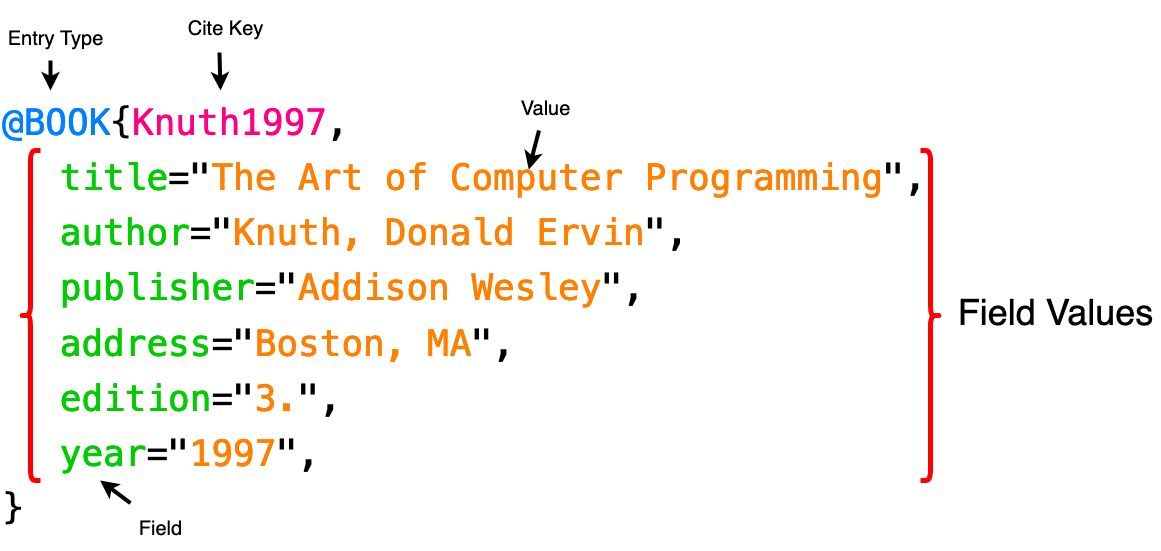
\includegraphics[width=0.8\linewidth]{diagrams/bibtexStructure.drawio.png}
    \caption{Structure of a BibTeX entry}
    \label{fig:bibTeXEntryStructure}
\end{figure}

The original BibTeX allowed only ASCII defined characters in its files. Following tools/versions have extended this to allow UTF-8, however I have made the decision to only allow ASCII characters within my system (non ASCII characters are disregarded - to prevent them crashing the system). This may seem like a backward step, however as we will see it is important for the efficiency of the key string matching algorithm we will implement, and thus important for keeping our application snappy and easy to use. BibTeX also already allows many common non-ASCII characters to be used such as accented characters through its default syntax \citep{bibtexSpecialCharacters}.

\subsubsection{Validity Checking}
The simple format of the files meant we could do some pre-processing checks to ensure that a BibTeX entry is valid. As will be discussed in the following section an erroneous entry if not too drastic doesn't result in a rejection of the whole file, but can result in that entry being rejected and the error being notified to the user.

A few very simple checks can be done to make sure that an entry is valid:

\begin{itemize}
    \item Each entry must have an equal number of left curly brackets and right curly brackets (unless any individual curly bracket is escaped by a backslash)
    \item Each entry must have an equal number of quotations (notably double quotations, as this is necessary in the BibTeX format).
\end{itemize}

As said relatively few lines can be used to accomplish these checks (figure \ref{fig:equalCurly}). 
\begin{figure}
    \centering
    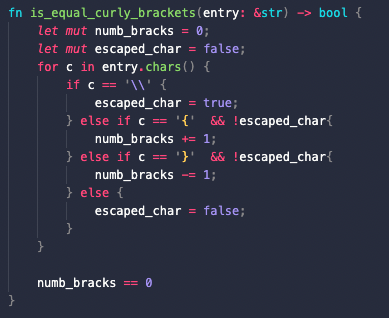
\includegraphics[width=0.5\linewidth]{images/equalCurlyBrackets.png}
    \caption{Code to determine if an entry has equal left and right brackets.}
    \label{fig:equalCurly}
\end{figure}

\subsection{Parsing}
Due to the relatively simple syntax of the files the approach taken to parsing and dealing with nuances in these files was relatively simple. To parse the files a combination of more naive, string splitting techniques was used, as well as a more sophisticated, character consumer based approach. The simple, consistent structure of bibtex files made the splitting technique viable, but the more nuanced intricacies of the individual field entries made the character consumer also necessary. 

The parser being developed had to be error proof/prone such that it could recover from relatively simple errors. This was important as many BibTeX files could be hundreds of entries long, and we don't want a single erroneous entry to prevent the parse and dealing of the rest of the entries in the file.

Therefore the first step was, as much as possible, to break the file's string into an array of strings, each string containing one bibtex entry. Due to the '@' symbol being a special reserved character in BibTeX which marks the beginning of a entry (unless escaped), this was a simple operation to perform.

\subsection{Core Parsing Technique}
Once dealing with individual entry strings, we must use a more generalised technique to ensure correct parsing of individual components. Referring back to figure \ref{fig:bibTeXEntryStructure} we can tokenise the structure of a BibTeX entry. Knowing this, we can build a character consumer which can iterate through the entry and produce these tokens, much as in the style of a top down parser. In order to produce this, I created a state machine which handles the input stream of characters (figure \ref{fig:stateMachine}).

\begin{figure}[H]
    \centering
    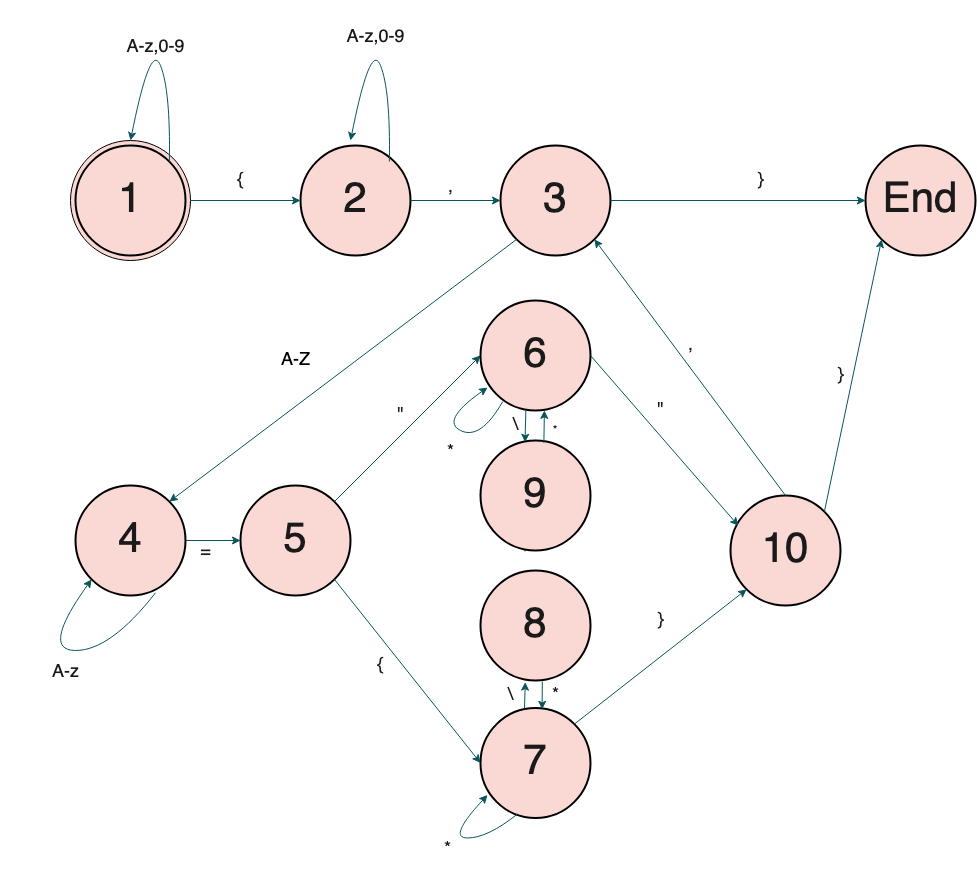
\includegraphics[width=\linewidth]{diagrams/dissStateMachine.drawio.png}
    \caption{State machine for the parsing of BibTeX Entries}
    \label{fig:stateMachine}
\end{figure}

In our project code we can use this to decide how to process each character in the input stream from the entry string. If we apply the colours from figure \ref{fig:bibTeXEntryStructure} to the state machine, we can see how the state machine was designed such that different areas are responsible for handling different 'tokens' in the BibTeX entry. These colours can be seen applied in figure \ref{fig:stateMachineColored}.

\begin{figure}[H]
    \centering
    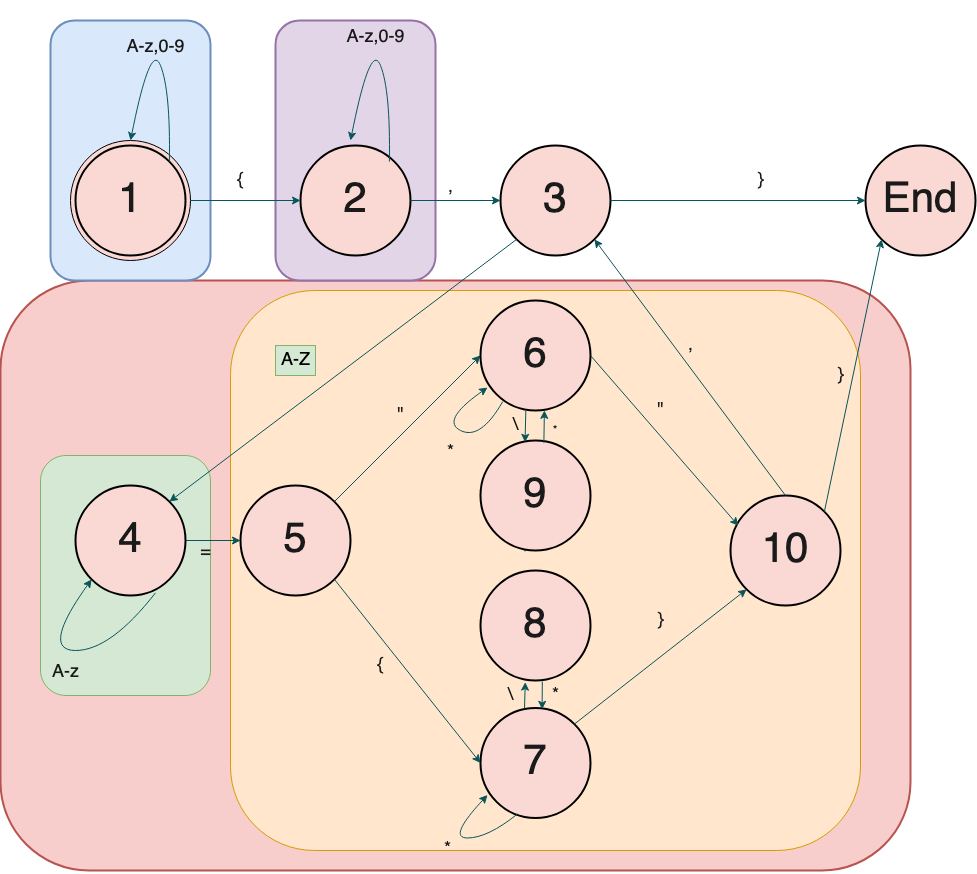
\includegraphics[width=\linewidth]{diagrams/dissStateMachineColorCoded.drawio.png}
    \caption{State machine for the parsing of BibTeX Entries color coded to match tokens in figure \ref{fig:bibTeXEntryStructure}}
    \label{fig:stateMachineColored}
\end{figure}

Within each 'state' in this machine a decision of what to do with the current character is decided. We can see an example of this; states eight and nine are the 'escaped character' states. These states are only reached following a backslash character. States six and seven, on receiving a quotation or right curly bracket respectively, will move to state ten, essentially ending the value for that key-value pair. In contrast states eight and nine will allow this character and process it as if it were any other character in state six and seven; 'escaping' the character.

This state machine abstracts over some of the details of a correct BibTeX file, such as the equal number of curly brackets and quotes, or the valid list of possible field names and entry types. However, by applying this machine in conjunction with the relatively simple pre-processing checks described above, we can ensure that the file is parsed correctly.

\subsubsection{Implementing the Parsing}
There is little to talk about the process of transforming the above described parsing method into rust code. The rust standard library provides plenty of in built functions to aid in this process and allow easy iteration of the characters within the entry. The parsed entry is put into a \code{BibEntry} struct with the following structure
\begin{minted}{rust}
pub struct BibEntry {
    pub entry_type: String,
    pub name: String,
    pub fields: Vec<Field>,
}
pub struct Field {
    pub field_name: String,
    pub field_value: String
}
\end{minted}
The parsed result of a file is a vector of \code{BibEntry} structs where each entry is a successfully parsed entry within that file. On library calls where more than one file is parsed, these parsed files are combined into a single aggregated Vector of all the successfully parsed structs. This will later allow any duplicates across files to be identified, as well as any duplicates within the same file. 

\subsubsection{Error Handling}

Abstracting the parsing method for entries into a state machine makes error handling and recovery particularly easy. Once the pre-emptive checks are done on the entry, we know that if it succeeds in travelling through the state machine to the end state then that BibTeX entry is a correct one. Through the state machine, an error can be detected if a character is entered for which their is no output from that state. For example in state five (figure \ref{fig:stateMachine}) if the following character is neither '"' or '\{' then we have entered an erroneous state, and can report that entry as improperly formatted.

A benefit of having already broken the file into the separated entries is that if the state machine fails for a given entry, it doesn't prevent the rest of the entries in the file being parsed. Therefore a broken entry won't necessarily break the rest of the file from being parsed and used.

If an error is identified which is unrecoverable this is often managed through the \code{Neon::Result<T>} struct, which will throw the error back up to the Javascript run time. Therefore this error is still notified to the user, who can gracefully handle it at the client side. All parsing functions are library function calls in a separated thread from the main GUI as we will see later, therefore asynchronous function calls to my rust library won't disrupt the users application usage even if there is an error present.

\subsection{Matching BibTeX Entries}
This section examines how the application goes about determining two near similar BibTeX entries using smart approximate string matching techniques. Identifying matching BibTeX entries correctly in this context is crucial; false negative matches will result in duplicate entries remaining within the file (less hazardous), false positives matches could result in a non-duplicated BibTeX entry being removed. The latter of these is very hazardous as it could destroy work of the author - resulting in even more work recovering the lost citation.

Approximate String matching algorithms return some score result defining the distance or number of operations between two strings. This score denoted as $s$. The final choice of algorithm will have a normalised value for $s$ where where $0 < s < 1$. We say that if $s == 1$ then the distance between these two strings is infinite (an unobtainable case), if $s == 0$ then the strings must be identical. Using this, we can define some threshold $t$ below which we can mark the two entry strings to be similar enough to be identified as duplicates.

The value of $t$ we choose is vital to this applications success, too large a value and we will get a large number of false positives. Too small a value and we shall incorrectly reject true duplicates. The latter of this is the preferred case, as this does not at best inadvertently destroy the authors work, however one of the main intents of this application is to remove duplicates so choosing this value poorly still defeats the goal.

Extended beyond this, choice of algorithm is not the only key to correctly identifying duplicates. We must also examine the details of each BibTeX entry in order to properly understand what identifying factors help eliminate duplicates.

First of all, we can eliminate certain tokens from the entry from being used in the duplicate search.
\begin{itemize}
    \item The entry type will be repeated between completely different citations, so should not be examined in the entry comparison.
    \item The entry reference key is essentially a random string created by the author or some citation generator, which holds no relevance to the rest of the citation. Two completely unrelated citations may hold extremely similar reference keys, so utilising this value could in fact increase our false positive rate (see figure \ref{fig:similarReferenceKeys}).
    \item Other fields which are not unique to any single BibTeX entry. Examples of such fields include \code{year}, \code{volume}, \code{journal} or \code{month}.
\end{itemize}

\begin{figure}
\centering
\begin{subfigure}{.5\textwidth}
  \begin{minted}{rust}
@article{citation1,
  author   = "Anne Baker",
  title    = "Example A",
  year     = 1999,
  volume   = "50",
  number   = "6",
  pages    = "1143--1148",
}
\end{minted}
\end{subfigure}%
\begin{subfigure}{.5\textwidth}
  \begin{minted}{rust}
@article{citation2,
  author   = "John Smith",
  title    = "Example B",
  year     = 1999,
  volume   = "20",
  number   = "3",
  pages    = "1143--1144",
}
\end{minted}
\end{subfigure}
\caption{Two unrelated citations with very similar reference keys and other fields}
\label{fig:similarReferenceKeys}
\end{figure}

In fact it turns out that no single field on its own can uniquely identify a citation; authors, or combinations of authors may have done several research papers (which will very often be cited within the same article), and, although unlikely, two citations could theoretically still share the same title. The only way to reliably uniquely identify a citation is to use the author and title in conjunction with each other.

There are other fields which could be brought into this grouping, such as the abstract of a paper, but this is excluded from the duplicate comparison as it is a very long string (slowing down the algorithms and hence response time), and is also often not included in the citation at all. In contrast the title and author are fields present in nearly all citations.

The difference between two identified near duplicates can come in one of two forms.
\begin{enumerate}
    \item Due to a 'typo' in either of the strings.
    \item Due to different formatting styles in each field; either due to different generators, or different methods of capitalising characters/words in the string or different formats in the author field.
\end{enumerate}
Both are common, but the second is more complex to deal with and requires more complex algorithms for identifying such a case. The latter arises due to curly brackets being used to ensure capitalisation of words within a title. See figure \ref{fig:differentButSameTitles} for an example of two equivalently-outputted title fields with varying values.

\begin{figure}[H]
\centering
\begin{subfigure}{.5\textwidth}
  \begin{minted}{rust}
title="The Life of {Albert} {Einstein}"
\end{minted}
\end{subfigure}%
\begin{subfigure}{.5\textwidth}
  \begin{minted}{rust}
title="The Life of {A}lbert {E}instein"
\end{minted}
\end{subfigure}
\caption{Two title fields of same citation, with same output, but different values}
\label{fig:differentButSameTitles}
\end{figure}

Similarly, the 'and' word is a reserved keyword within author fields, and is used to delimit different authors names. A comma in the author field is also used to separate last and first name. Both of these can be escaped within an author field by embracing them within curly brackets. As a result it is possible to have multiple values for an author field result in the same output, see figure \ref{fig:differentButSameAuthors}. These are all possibilities we must consider when choosing our approximate string matching algorithm.

\begin{figure}[H]
\begin{subfigure}{\textwidth}
    \begin{minted}{rust}
    author="Jung, Ralf and Jourdan, Jacques-Henri and Krebbers, Robbert and Dreyer, Derek"
    \end{minted}
\end{subfigure}
\begin{subfigure}{\textwidth}
    \begin{minted}{rust}
    author="{R. Jung} and {J.-H. Jourdan} and {R. Krebbers} and {D. Dreyer}"
    \end{minted}
\end{subfigure}
\begin{subfigure}{\textwidth}
    \begin{minted}{rust}
    author="Ralf Jung and Jacques-Henri Jourdan and Robbert Krebbers and Derek Dreyer"
    \end{minted}
 \end{subfigure}  
 \begin{subfigure}{\textwidth}
    \begin{minted}{rust}
    author={{R. Jung, J.-H. Jourdan, R. Krebbers, and D. Dreyer}}
    \end{minted}
 \end{subfigure}   
 \caption{Four author fields with different formatting but same output}
\label{fig:differentButSameAuthors}
\end{figure}

We can see that the author fields in figuer \ref{fig:differentButSameAuthors} have very different character structures, and normally different ordering of words. A simple algorithm which only evaluates basic character operations would give a difference value which would indicate a much higher difference between the strings than is actually truthful. We will see the different matching algorithms that attempt to solve this issue.

\subsection{Matching Algorithms}
The context surrounding existing matching algorithms is already extremely extensive, with hundreds of different approximate string matching algorithms having been developed. Therefore the goal of this project was not to decipher which algorithm is overall the best, but rather to explore a subset of existing ones with increasing complexity in order to understand the range of techniques used within this field. Then, using this information decide which algorithm of the ones experimented with is best within the context of our application.

In this work I examine 6 different, varying complexity algorithms:
\begin{enumerate}
    \item \textbf{Hamming Distance}
    \item \textbf{Levenshtein}
    \item \textbf{Damerau Levenshtein}
    \item \textbf{Jaro-Winkler distance }
    \item \textbf{An N-Gram based distance algorithm}
    \item \textbf{A string space to vector space algorithm (Jensen Shannon).}
\end{enumerate}

In the following sections I will examine each algorithm and their relevance and usefulness in this context. All of the algorithms can be tested in the 'Algorithm Sandbox' tab of the final application.

\subsubsection{Hamming Distance}
Throughout the different algorithms we will continuously hear the notion of edit distance between two strings. The edit distance between two strings is described as the number of atomic operations required to convert one string into another string. Hamming distance is the first and simplest algorithm which uses this notion to describe the 'distance' between two strings. Originally, hamming distance was referenced in the context of \textit{codewords}, where the hamming distance between two codewords is simply the number of bit positions in which they differ \citep{hammingDefinition}. 

This can be generalised to the context of strings where we redefine it to be the number of edits required to tranform a string to another string of equal length. In this metric the only edit operation allowed is 'substitution' where one character is swapped for another. We will see how further algorithms extend upon this by adding in more operations.

\begin{figure}[H]
    \centering
    \begin{minted}{rust}
    // assumes same length strings
    pub fn hamming(str1: &str, str2: &str) -> i32 {
        let mut count = 0;
        for (i, c_1) in str1.chars().enumerate() {
            let c_2 = str2.chars().nth(i).unwrap();
            if c_1 != c_2 {
                count += 1;
            }
        }
        
        count
    }
    \end{minted}
    \caption{Hamming Distance implemented in Rust}
    \label{fig:hammingImplemented}
\end{figure}

For our application this algorithm is too simple and as such is not suited. Particularly as the hamming distance is only able to operate on strings of same length (unless the shorter string is extended with additional special characters to match the longer strings length, although this is not in the faith of the original algorithm). The hamming distance, as many of the following algorithm, also provides an integer output corresponding to the number of operations required to match the strings. This output, $d$, has a value given input strings of $s_1$ and $s_2$ where $len(s_1) = len(s_2)$ of at minimum 0, should $s_1 == s_2$, or at most $len(s_1)$. This integer output will give a distance definition between the strings which is associated with the input strings themselves. For the context of our application it would be far more suitable to have some bounded metric be output independent of the original algorithm input. Although it would be possible to create a function to bound the hamming output given its input contexts, further algorithms we explore are designed with this intent.

Although a simple operation, this algorithm stills finds usability today, particularly in more restricted contexts such as signal error handling. In this context we can say that if the Hamming distance between two codewords $c_1$ and $c_2$ is $d$, and $c_1$ is transmitted, then $d$ errors would have to occur for codeword $c_2$ to be received \citep{hammingDefinition}. In the context, one the key benefits of this algorithm is its complexity. As can be seen in figure \ref{fig:hammingImplemented} we get a very simple implementation with very low complexity; with worst case ${O}(n)$ performance. As we will see in later examples, sometimes this complexity must be sacrificed for accuracy of each algorithm.
% complexity discussion

\subsubsection{Levenshtein Distance}
Levenshtein is another extension on edit operations to the hamming distance metric. Levenshtein distance is often informally known as ``edit distance", although this is often too vague as edit distance may refer to the larger family of edit metrics which we will see in other algorithms. It was originally proposed in 1965 by Russian mathematician Vladimir Levenshtein \citep{levenshtein1965binary}, and extended hamming distance by allowing insertions and deletions, as well as subtitutions.

Formally, the levenshtein distance between two strings $a$ and $b$ where $|a|$ is the length of string a, is defined as.

\begin{equation}
    lev(a,b)= \left\{\begin{matrix}
 |a| & if |b|=0\\ 
 |b| & if |a|=0\\ 
 lev(tail(a), tail(b))& if a[0]=b[0] \\ 
 1 + min\left\{\begin{matrix}
lev(tail(a),b)\\ 
lev(a,tail(b))\\
lev(tail(a),tail(b)) 

\end{matrix}\right.& otherwise 
\end{matrix}\right.
\end{equation}

Note that in the above, each operation is represented by a certain recursive call.
\begin{itemize}
    \item $lev(tail(a), b)$ represents deletion (from a to b)
    \item $lev(a, tail(b))$ represents insertion (from a to b)
    \item $lev(tail(a), tail(b)$ represents substitution.
\end{itemize}

An important note of this algorithm is due to the addition of the insertion (and deletion) operations, strings in the algorithm no longer had to be the same length; a step towards its usability within our application. The addition of these operations creates some interesting properties.

First of all the upper and lower bounds on distance between two strings change. The lower bound is now the difference in length between the two strings $d_{min} = MOD(|a| - |b|)$. The upper bound is now the length of the longer string $d_{max} = MAX(|a|, |b|)$. Interestingly, if the strings are the same length then the upper bound on the distance is equivalent to the hamming distance between the two strings. However, this does not mean that two strings of equal length will have equivalent hamming and levenshtein distance. For example, take the strings ``print" and ``rinse". The levenshtein distance between these two strings is 3 (figure \ref{fig:levenshteinDemo}), whereas the Hamming distance between these two strings is 5. We can see from this how levenshtein is a step closer to achieving a more realistic sense of how similar two words are.

\begin{figure}[H]
    \centering
    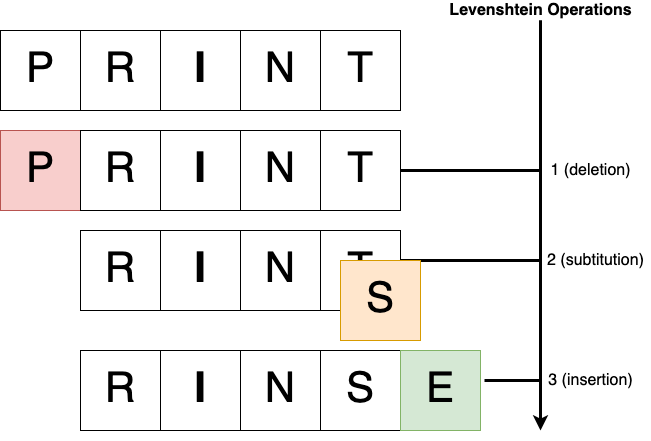
\includegraphics[width=0.4\linewidth]{diagrams/levenshteinDemo.png}
    \caption{Levenshtein operations to transform "print" into "rinse"}
    \label{fig:levenshteinDemo}
\end{figure}

% two implementations
There are two methods of implementing the algorithm. The first is a more naive, but simpler to understand recursive based algorithm. In this algorithm (figure \ref{fig:levenshteinRustImplementation}) we see how, as in the formal definition, after a comparison of the characters at the at the current indices, we attempt to apply each of the three operations to the tail of the string. This becomes inefficient rapidly due to to repeating the same levenshtein calculations on the same substring many times. It is easy to see from here how the algorithm would benefit from a dynamic programming/memoization implementation. A bottom-up dynamic programming algorithm for levenshtein distance was proposed by Robert A. Wagner and Michael J. Fischer in 1974 \citep{wagnerFischer} (although multiple proposers have been cited).

\begin{figure}
    \begin{minted}{rust}
    pub fn compute(str1: &str, str2: &str) -> i32 {
        let m = str1.len();
        let n = str2.len();
    
        leven(str1, str2, m, n)
    }

    fn leven(str1: &str, str2: &str, m: usize, n: usize) -> i32 {
        if m == 0 {
            return n as i32;
        }
        if n == 0 {
            return m as i32;
        }
    
        let str1_char = str1.chars().nth(m-1).unwrap();
        let str2_char = str2.chars().nth(n-1).unwrap();
        
        if str1_char == str2_char {
            return leven(str1, str2, m - 1, n - 1);
        }
    
        return 1 + min_of_3(
            leven(str1, str2, m, n - 1),  // insert
            leven(str1, str2, m - 1, n),  // remove
            leven(str1, str2, m - 1, n - 1)  // replace
        ) as i32;
    }
    \end{minted}
    \caption{Implementation of Naive recursive levenshtein algorithm in rust}
    \label{fig:levenshteinRustImplementation}
\end{figure}

This algorithm works by generating a matrix for strings $a$ and $b$ of size $|a| \times |b|$, where each index in the matrix reserves the edit distances between all prefixes of the first string and all prefixes of the second \citep{wagnerFischer}. Doing so allows this value to be used in subsequent recursive calls, preventing the recomputation of these values. The return value for the algorithm is then the value in the bottom right of the matrix.

We can evaluate how drastically the performance of these two differs by timing how long each implementation takes to perform comparisons on the same, 12 character length randomized strings. The results of this can be seen in table \ref{fig:levenshteinResults}. We can see how exponentially quickly the running time of the recursive implementation increases; about a 25 second average computation time to compare two strings of only 12 characters in length! 

\begin{figure}[H]
\begin{center}
    \begin{tabular}{|c|c|c|}
    \hline
         Test Number & Levenshtein Recursive Time (ms) & Wagner-Fischer Time (ms) \\
         \hline \hline
         1 & 29617.756 &  0.229 \\ \hline
         2 & 27529.561 &  0.194 \\ \hline
         3 & 15981.572 &  0.188 \\ \hline
         4 & 28088.483 &  0.206 \\ \hline
         5 & 27100.224 &  0.195 \\ 
        \hline \hline
        Average & 25663.5 & 0.2024 \\
        \hline
    \end{tabular}
\end{center}
    \caption{Results of time based comparison of the two algorithms}
    \label{fig:levenshteinResults}
\end{figure}

Despite the memoization improvement offering significant optimisations over the recursive, we can see how quickly even the addition of two edit operations causes the complexity of the function to sky rocket. In particular it has been shown that all known algorithms for levenshtein distance run in near quadratic time, with the above algorithm running with complexity $O(n^2)$. Furthermore, it has been shown that if an algorithm was to run with complexity $O(n^{2-\delta})$ where $\delta$ is some constant where $\delta > 0$, then the satisfiability of conjunctive normal form formulas with $N$ variables and $M$ clauses would be able to be solved in time $M^{O(1)}2^{(1-\epsilon)N}$. If this were true this would violate the Strong Exponential Time Hypothesis. Therefore it can be concluded that such an algorithm does not exist \citep{levenshteinComplexityProof}.


To this date, despite large amounts of effort being undertaken to discover a lower complexity algorithm, the best achieved algorithm has a complexity of $O(\frac{n^2}{log^2n})$ for sequences of length $n$ \citep{fastestLevenshteinAlg}.

\subsubsection{Damerau-Levenshtein Distance}
Damerau Levenshtein is a further extension to the hamming distance and levenshtein distance algorithm, now inclusive of another operation; transposition of two adjacent characters. The original method was devised by Fred J Damerau in 1964 as a means to counter spelling errors and to aid spell checkers \citep{damerauLevenshtein}. Damerau suggests in this paper that it is common for miss spelt words not present in a dictionary to be wrong only via a missing or extra letter or a single transposition \citep{damerauLevenshtein}, so from this we can see the original domain for which this algorithm was devised for. Despite this, damerau levenshtein has found use in many of the other fields where approximate string matching algorithms have become ubiquitous, such as in genome sequence matching.

Once again, we can formally define the Damerau Levenshtein algorithm in a recursive fashion \citep{damerauLevenshteinDefinition}.

\begin{equation}
    d_{a,b}=min\left\{\begin{matrix}
0 & if i=j=0\\ 
1+ d_{a,b}(i-1,j) & if i> 0 \\ 
1+d_{a,b}(i,j-1) & if j > 0\\ 
1_{(a_i \ne b_j)} + d_{a,b}(i-1, j-1) & if i,j > 0\\ 
1+ d_{a,b}(i-2, j-2) & if i,j > 1 \land a_i = b_{j-1} \land a_{i-1}=b_j 
\end{matrix}\right.
\end{equation}

Like in the formal definition of Levenshtein distance, different steps in this formal definition represent different operations on the string. The new operation addition is represented by the recursive call on the last line of the definition. Note that the definition now uses character indexes rather than a \textit{tail(a,b)} function. This is necessary to easily denote the conditions necessary for a transposition to be possible.

Just as adding the two additional operations to Hamming distance increased the complexity of the algorithm from $O(n)$ to $O(n^2)$ time, there is another increase in complexity due to the addition of the fourth operation, transposition. Adding transposition adds such significant complexity in fact, that intermediate algorithms have been suggested which add additional constraints in an attempt to reduce this complexity. The first of these computes \textit{optimal string alignment distance or restricted edit distance}, rather than the true Damerau Levenshtein distance \citep{damerauLevenshteinDefinition}. This algorithm constrains the operations by adding the condition that no  \textit{substring is edited more than once}.

The implementation of this algorithm is an extension of the above Wagner Fischer dynamic programming algorithm, which adds the final transposition as a fourth operation to check.

The true algorithm requires an additional parameter, $\epsilon$, which is the size of the alphabet of the input sets.

% TODO: talk about complexity

\subsubsection{Jaro-Winkler Distance}
The Jaro Winkler distance is a step away from the edit distance/operations style of string matching algorithms, and is the first algorithm we are examining which returns a metric value between 0 and 1 describing the similarity of two strings. It works by searching for common characters between the strings and, like Damerau-Levenshtein, then examines the number of transpositions in the string. These values are then used to compute an output value describing the similarity of the strings.

This similarity function is defined as follows, given input strings $a$ and $b$ \citep{jaroDescription}

\begin{equation}
    jaro(a,b) = \left\{\begin{matrix}
0 & if m=0\\ 
\frac{1}{3}(\frac{m}{|a|} + \frac{m}{|b|} + \frac{m-t}{m}) & otherwise 
\end{matrix}\right.
\end{equation}

Where 
\begin{itemize}
    \item $|a|$ is the length of input string $a$
    \item $m$ is the number of matching characters, where $a_i$ and $b_j$ are considered matching only if
    \begin{equation}
        a_i == b_j
    \end{equation}
    and
    \begin{equation}
        mod(i - j) \leq \left \lfloor \frac{max(|a|,|b|)}{2} \right \rfloor - 1
    \end{equation}
    \item $t$ is the number of transpositions. This can also be calculated by counting the number of matching characters (with different sequence order) divided by two.
\end{itemize}

See figure \ref{fig:jaroDemo} for an example of how this works.

\begin{figure}[H]
    \centering
    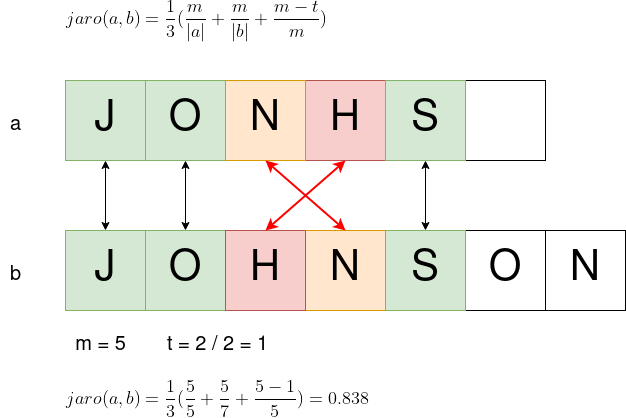
\includegraphics[width=0.7\linewidth]{diagrams/jaroDemo.drawio.png}
    \caption{Demonstration of how the Jaro distance is calculated}
    \label{fig:jaroDemo}
\end{figure}

Jaro-Winkler distance is an extension of this which works under the assumption that the first few letters of the string, some prefix $p$, are the most 'important' few letters of the string. This is done by ``boosting" the score by some amount proportional to the rest of the score. This is defined as follows \citep{jaroWinklerOriginalPaper}
\begin{equation}
    jaroWinkler(a,b) = jaro(a,b) + lp(1-jaro(a,b))
\end{equation}

Where 
\begin{itemize}
    \item $jaro(a,b)$ is the jaro similarity score for strings $a$ and $b$
    \item $l$ is the length of the common prefix at the start of the string with \textbf{a maximum value of four characters}
    \item $p$ is a constant scaling factor. 
\end{itemize}

Increasing the constant factor $p$ means the score is increased more for having common prefixes in the first four letters. This value is such that $0 < p < 0.25$. 0.25 is the threshold as exceeding this value could result in scores greater than 1, due to the max of a four letter prefix (although there is no reason this could not be changed for different contexts). Winkler in his original work uses the value 0.1 \citep{jaroWinklerOriginalPaper}, which is what is used in this applications implementation.

An important note on Jaro-Winkler distance is that although colloquially referred to as a distance 'metric', formally speaking this algorithm is not a metric. This is as it does not obey the triangle inequality \citep{jaroWinklerTriangleLaw}. This law states that if found some metric between strings A and B, and applied the same metric between strings B and C, then there would be a relationship between these results and the results of the same metric applied between A and C. Jaro Winkler does not obey this law, and whilst this may be unimportant for our context, it means that this technique ``cannot be used to embed strings in a metric space" \citep{jaroWinklerTriangleLaw}, a method which some other approximate string matching techniques use to leverage a similarity score.

\subsubsection{N-Gram}
For understanding the N-gram based algorithm, it is first simplest to understand the notion of Longest Common Subsequence (LCS), and how it can be applied itself as an approximate string matching metric. A subsequence of a set can be described as a sequence of characters which is a subset of the original set, which maintains the order of characters in the original set. This can be derived from a given sequence by deleting some or no elements without changing the order of the remaining elements. For example $\{A,B,C\}$ would be considered a subsequence of the set $\{A,D,B,C,E\}$.

From this we can formally define the LCS of two strings $X[1..m]$ and $Y[1..n]$.
A subsequence, $S[1..s]$ is obtained by deleting $m-s$ symbols from $X$. A common subsequence of $X[1..m]$ and $Y[1..n]$ is a subsequence which can be found in both of the strings. The longest common subsequence of the two strings is simply the common subsequence of the two strings with the longest length \citep{lcsFormalDefinition}.
For example the LCS between the strings ``natural" and ``contrary" is ``ntra".

This alone is a simple distance metric which can be used for approximate string matching. This said, G. Kondrak \citep{ngramDistanceImplementation} in his paper describes how LCS is problematic due to its insensitivty to context (see figure \ref{fig:lcsExample}) for an example).

\begin{figure}[H]
    \centering
    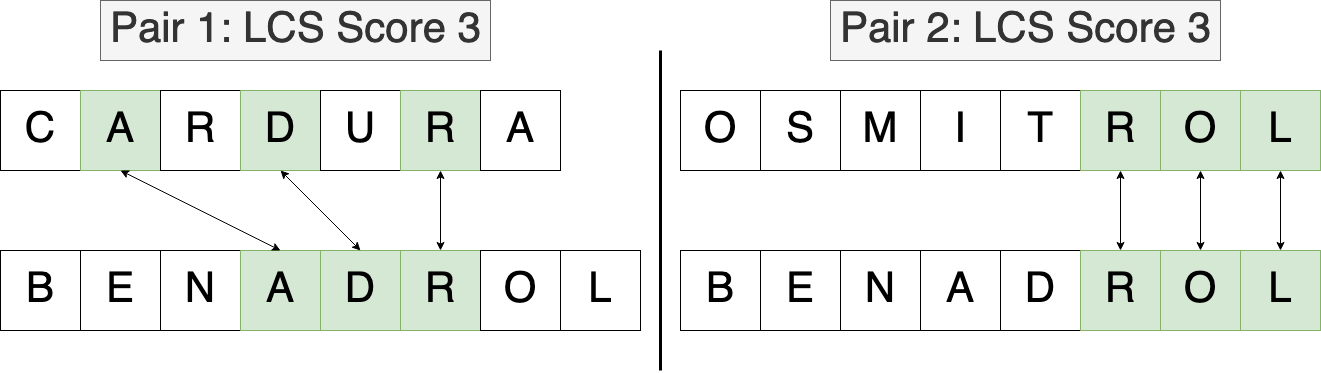
\includegraphics[width=0.9\linewidth]{diagrams/LCSUnrelatedStrings.drawio.png}
    \caption{Pair of words with the same length of longest common subsequence, example cited from \citep{ngramDistanceImplementation}}
    \label{fig:lcsExample}
\end{figure}

We can see in the figure \ref{fig:lcsExample} how despite pair two (right) appearing much more similar, especially given surrounding context of the words, this metric still returns the same score for both pairs. This example shows that parallel identity matches are a much stronger indication of similarity than matches that are separated by unmatched symbols \citep{ngramDistanceImplementation}.

An n-gram based distance algorithm, known as DICE, was designed to in part solve this problem. A $n$-gram within some string $S$ can be defined as any $n$-long subsequence of consecutive tokens. The ith $n$-gram of $S$ is the sequence $(s_i, s_{i+1}, ..., s_{i+n-1})$  \citep{ngramBio}. The DICE measures are defined as follows \citep{ngramDistanceImplementation}
\begin{equation}
    \frac{2 \times | ngrams(X) \cap ngrams(Y)|}{|ngrams(X)| + |ngrams(Y)|}
\end{equation}

This ratio attempts to solve the problems described of LCS as it provides location dependent context to the LCS algorithm by examining characters which are next to each other rather than individuals. This said, DICE comes with its own problems; n-grams can be restrictive as many very similar words can share no or few $n$-grams in common; for example ``mini" and ``mono" share no 2-grams. The measure still has context imperfections, as the ratio doesn't take into account the location of the n-grams compared, even if two identical n-grams are in radically different positions within the string \citep{ngramDistanceImplementation}.

This brings us to the algorithm implemented within this project, derived from the work by Grzegorz Kondrak in his paper \textit{N-Gram Similarity and Distance }\citep{ngramDistanceImplementation}. As stated by Kondrak, ``the main idea behind $n$-gram similarity is generalizing the concept of the longest common subsequence to ecompass $n$-grams, rather than just unigrams" \citep{ngramDistanceImplementation}.

To do this, we first define a recursive definition of the longest common sequence. $s(X,Y)$ denotes the LCS between strings $X$ and $Y$. For this recursive definition, a notational shorthand is introduced, borrowed from Smyth \citep{computingPatternsInStrings}. Let the following be a pair of prefixes of strings $X$ and $Y$.
\begin{equation}
    \Gamma_{i,j}=(x_1...x_i, y_1...y_j)
\end{equation}
The following is a pair of suffixes from strings $X$ and $Y$
\begin{equation}
    \Gamma_{i,j}^*=(x_{i+1}...x_k, y_{j+1}...y_l)
\end{equation}
For strings of length one or less, we can state the follwoing.
\begin{itemize}
    \item $s(x, \epsilon)=0$
    \item $s(\epsilon,y)=0$
    \item $s(x,y)=\left\{\begin{matrix}
1\; if\; x = y\\ 
0\; otherwise

\end{matrix}\right.$
\end{itemize}

Where $\epsilon$ denotes an empty string.
From this, for longer strings, $s(X,Y)$ can be defined as follows \citep{ngramDistanceImplementation}.
\begin{equation}
    s(X,Y) = s(\Gamma_{k,l})=s(\Gamma_{i,j})+s(\Gamma^*_{i,j})
\end{equation}

We can then modify this definition slightly, as well as our notation for $\Gamma$ to encompass ngrams. We now require $\Gamma_{i,j}$ and $\Gamma_{i,j}^*$ to contain at least one complete $n$-gram. Now, referring back to the following statements we made about strings of length one or shorter, we can apply similar thinking to the $n$-gram definition. This now refers to a pair of strings which contain only one complete $n$-gram in either of the strings; now the $n$-gram similarity must be zero.

Let $\Gamma^n_{i,j}=(x_{i+1}...x_{i+n}, x_{j+1}...x_{j+n})$ be a pair of ngrams in X and Y. If both strings contain exactly one $n$-gram, it is easy to see that the output n-gram similarity is binary; either one if the $n$-grams are identical, or zero otherwise. For longer strings, we can once again define $n$-gram similarity recursively \citep{ngramDistanceImplementation}.
\begin{equation}
    s(X,Y)=s_n(\Gamma_{k,l})=s_n(\Gamma_{i+n-1, j+n-1}) + s_n(\Gamma^*_{i,j})
\end{equation}

From this we can easily derive a recursive algorithm for the computation of $n$-gram similarity. We can normalise the output of this by dividing the similarity score by the length of the input string with the longest length (in our case we subtract this from one to be consistent, such that 0 is an exact match). In my implementation, we use an extension of the dynamic programming algorithm from the LCS implementation. We can see how similar the recursive definitions of these two algorithms are, so extending the dynamic programming LCS algorithm to use $n$-gram matching instead is not too arduous a task.

We can perform some complexity analysis on this algorithm to further understand the running costs, which we can later examine when choosing our algorithm. Examining the algorithm itself we can give the algorithm a complexity; given two strings with respective lengths $m$ and $n$, the algorithm has a complexity of $O(mn)$. Meaning the algorithm is quadratic in complexity given two strings of the same length. We can examine this further by testing its computation time for increasing lengths of strings, the results of this can be seen in figure \ref{fig:ngramComplexityAnalysis}.

\begin{figure}
    \centering
    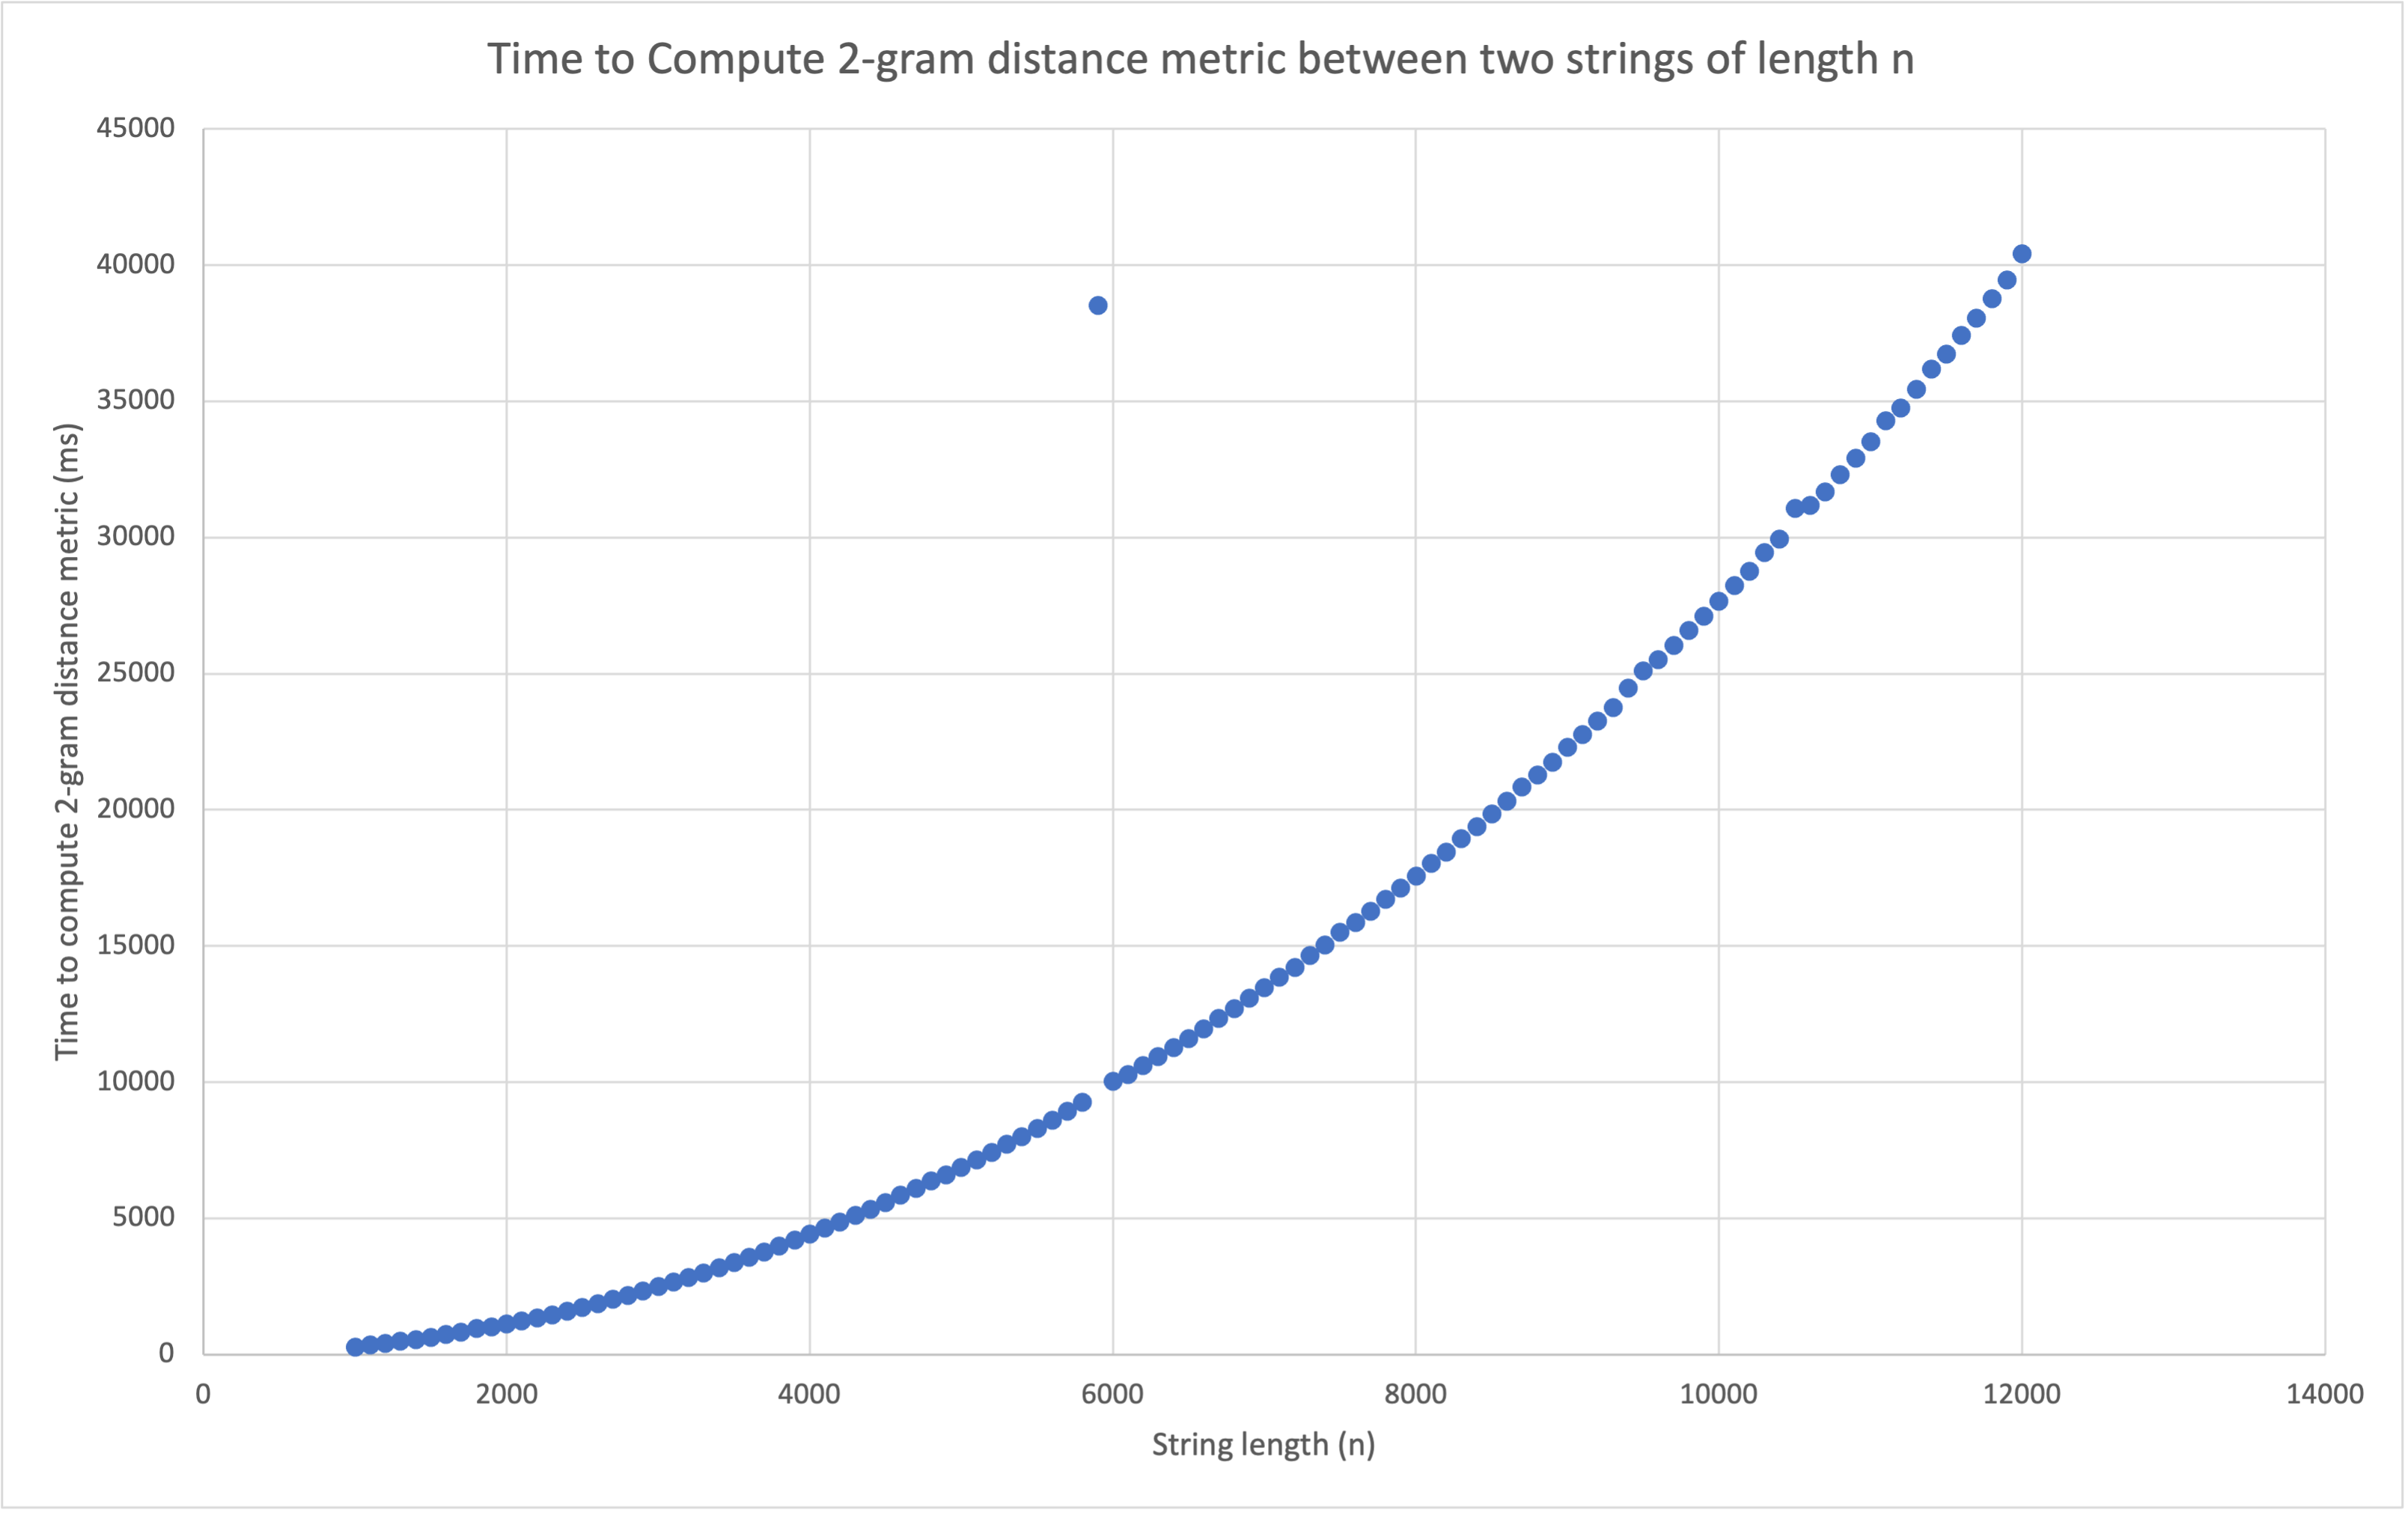
\includegraphics[width=0.8\linewidth]{diagrams/ngramComplexity.png}
    \caption{N-Gram distance Complexity Analysis}
    \label{fig:ngramComplexityAnalysis}
\end{figure}

From figure \ref{fig:ngramComplexityAnalysis} we can see a clear quadratic shape to the graph, indicating our understood quadratic time complexity of the algorithm.

This is the most complex algorithm we have described so far, and we will see this reflection in its applicability more in the 'Choice of Algorithm' section of the report. This algorithm no longer views only single character operations but now instead takes into account combinations of character adjacent sub sequences ($n$-grams) to create a defined score, essentially allowing it to more mathematically view the context in which characters sit in relation to characters in the other string.

\subsubsection{Jensen Shannon}
The work of this algorithm is derived from my supervisor, Richard Connor et al and their work on applying Jensen Shannon Distance over strings \citep{richardsPaper}. This technique itself is ``derived from a distance metric defined over labelled trees", the more detailed description of which can be found in \citep{jensenShannonTrees}.

In this technique, we devolve each string into its individual characters and digrams (2-grams). Each of these of these is known as an `event' and is assigned some frequency according to its number of appearances in the string. To add to this, notional start and finish characters are prefixed and suffixed to the string, denoted as $\phi$ and $\omega$ respectively. Table \ref{table:mumTable} shows the characters and digrams of the string ``mum", alongside their relative frequencies.

\begin{table}[]
    \centering
    \begin{tabular}{|c|c|}
\hline
    Character/Digram & Relative Frequency \\
    \hline
    ``$\phi$m" & 1/6\\ 
    ``mu" & 1/6\\ 
    ``um" & 1/6\\ 
    ``m$\omega$" & 1/6\\ 
    ``m" & 1/3\\ 
    ``u" & 1/6\\
    \hline
\end{tabular}
    \caption{Characters and Digrams of the string ``mum" alongside their relative frequencies}
    \label{table:mumTable}
\end{table}

In a more formal sense, the technique uses di-gram shingling to transform each character of a string into a very high-dimensional probability space, where individual characters and character di-grams are represented as a different event. As a result, if our character set is 127 characters in length, then the space will comprise of $127^2 + 127$ different possible events \citep{richardsPaper}.

To give us a metric on string similarity, Jenson-Shannon distance is then applied over this probability ensemble. The Jensen Shannon distance between two probability vectors $x$ and $y$ can be defined as $jsd(x,y)=\sqrt{JSD(x,y)}$, where $JSD(x,y)$ is the Jensen Shannon divergence between the probability vectors. This is defined as \citep{richardsPaper}.
\begin{equation}
    JSD(x,y) = 1 - \frac{1}{2} \sum_i x_ilog_2x_i + y_ilog_2y_i - (x_i + y_i)log_2(x_i + y_i)
\end{equation}

To implement this algorithm we first need to convert each string into an array of relative probabilities of each of its digrams and characters. This is done through iterating through each character and constructing a map containing as keys each of the individual characters and digrams. Each time this character/digram is seen the value of that key in the map is incremented by some cardinality number (2 if single character, 1 if digram). This cardinality number is also added to a running total. Once this is finished, this map is finalised by iterating through each key, storing it as an event, then calculating its relative probability through dividing its value by the kept running total; this gives us the relative probability of each of our events in the string.

% TODO: how we store digrams

Once this is completed for both strings, we can simply apply the calculation for JSD distance we have seen above to calculate our metric for distance between the strings.

The work required to convert the string into a sparse probability array takes $O(n)$ time, requiring only a single iteration of the string. The latter work done to calculate the JSD distance between two strings requires iterating over all the events of each string. A string of length $n$ will, with prefixed and suffixed characters have a maximum number of $n+1$ possible digrams. As a result the maximum number of events possible for a given string is equal to $2n+1$. That said, this result is constrained by the character set (alphabet) that the string is from. Given an alphabet $\Sigma$ of size $|\Sigma|$, then the number of possible digrams in that character set is equal to $|\Sigma|^2$. As a result, a worst case JSD distance calculation will be constrained to iterating over a maximum number of $|\Sigma|^2 + \Sigma$ events. Therefore if we have a string $S$ with length such that $|S| > |\Sigma|^2 + |\Sigma|$ then more operations will be guaranteed to take place during the building of the sparse arrays. This said, both sections of the algorithm give $O(n)$ complexity, therefore this algorithm will complete in linear time; giving it a much lower complexity than other metrics such as levenshtein or even the $n$-gram based algorithm.

We can see this complexity in figure \ref{fig:jensenShannonGraph}, which plots the time taken in milliseconds to compute the Jensen Shannon metric against two random strings of length n.

\begin{figure}
    \centering
    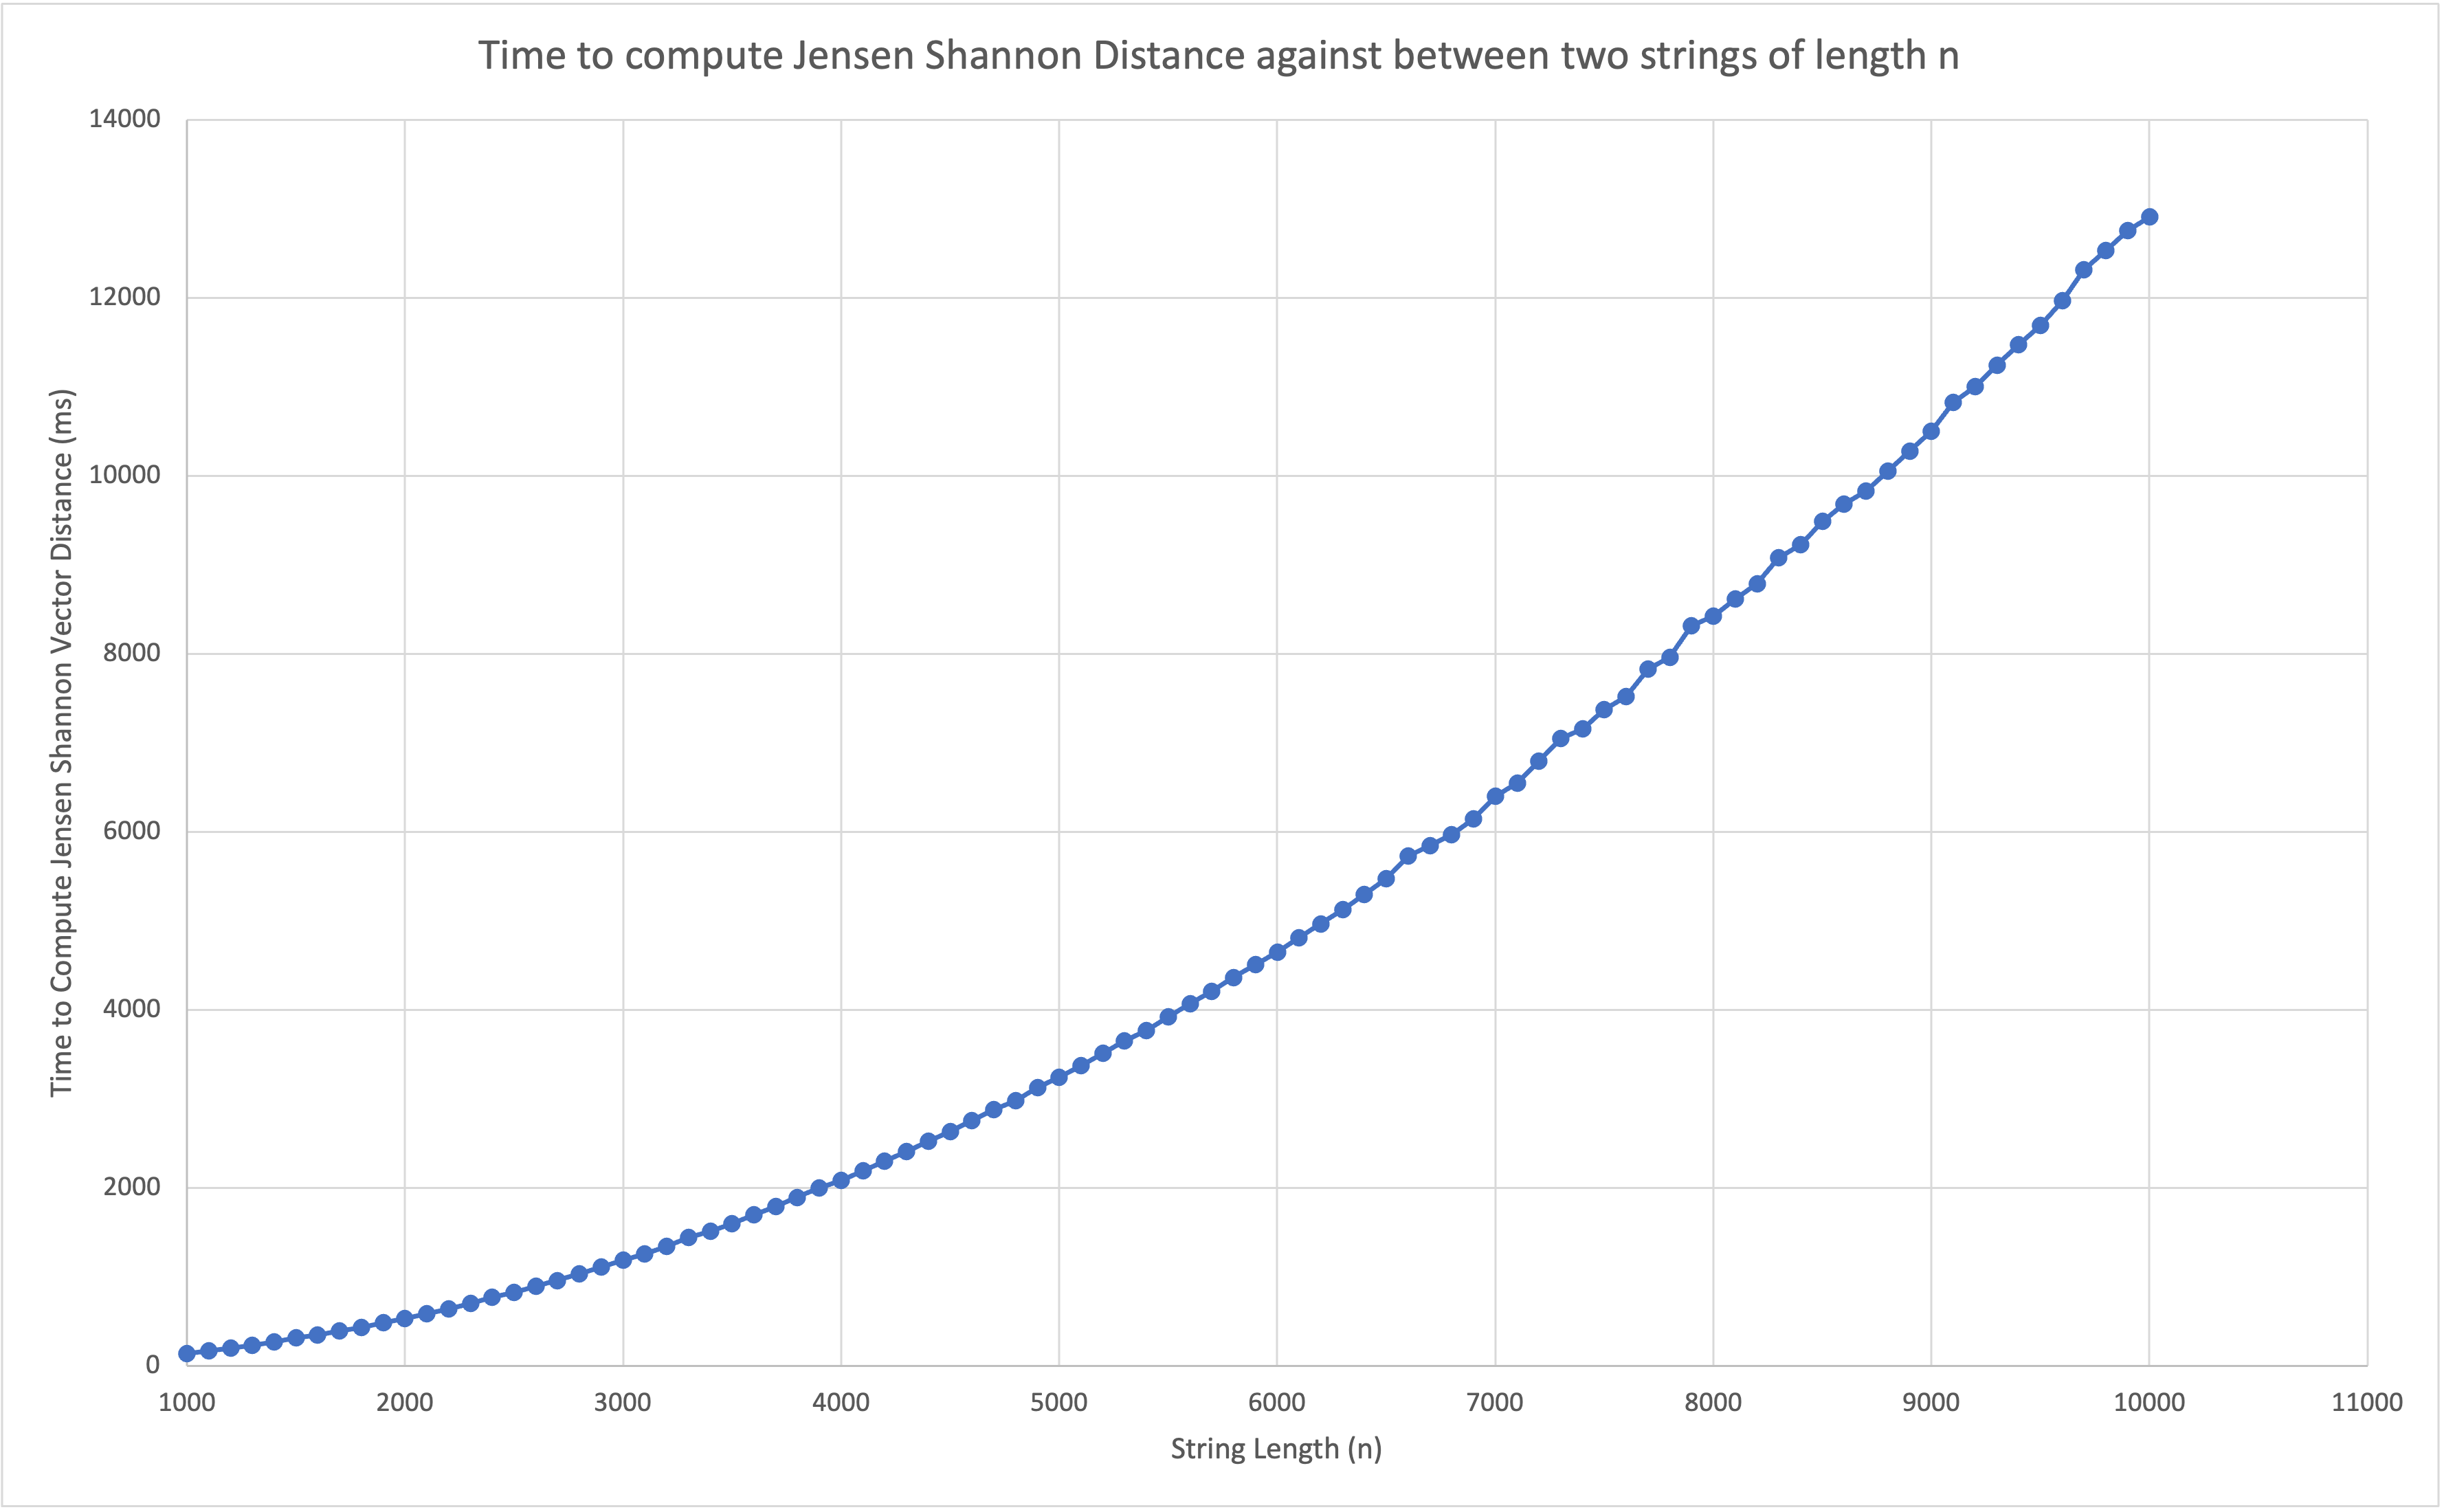
\includegraphics[width=0.8\linewidth]{diagrams/JensenShannonComplexity.png}
    \caption{Jensen Shannon Complexity Analysis}
    \label{fig:jensenShannonGraph}
\end{figure}

We can see in this figure that as the length of each string increases, post roughly 7000 characters the time taken to compute this algorithm seems to increase at a linear rate, confirming our thoughts. We also note that the time taken for this algorithm to compute a metric for strings of length 10,000 is roughly half that of the $n$-gram based algorithm.

The code for the implementation of this algorithm can be seen in the file \code{jensen\textunderscore shannon\textunderscore vector.rs}. This algorithm nicely rounds off those we implemented due to its combination of the use of $n$-grams, and statistical based methods; essentially combining the other work which we have analysed.

\subsection{Choice of Algorithm}
When choosing an algorithm, it was important to examine the context within which the algorithm would be being deployed, and hence to examine which is likely to fair best and produce the most accurate results.

In the section \textit{Matching BibTeX Entries} we have already discussed some of the possibilities for how the BibTeX entries we will be checking can vary, in this section we will take examples of these and apply several of the above algorithms to see how well they fair. Although this is an important factor in the final choice of algorithm, it is also important to examine the time each algorithm takes to perform such an analysis. The chosen algorithm may be called thousands of times for a single merge of two or more BibTeX files, so it is important that the complexity of the chosen algorithm also is not too high.

We can discuss the complexity of each of these briefly, but it is also worth noting that at the scales we are working at, the computational complexity may not be the best reflection to use in our context. A linear complexity algorithm may complete its operation on the relatively small sized strings we will be examining in a much greater time than a quadratic complexity algorithm. Therefore, the practical time of each algorithm must also be acknowledged.

To analyse the accuracy of the different algorithms I created small data sets for author and title, with groups of values which are similar in semantic (an example of such group is the example authors shown in figure \ref{fig:differentButSameAuthors}. Each of these sets then had Wagner-Fischer, Jaro-Winkler, $n$-gram and Jensen-Shannon applied to them with the results and timing data recorded. This data and timing/score results can be found in the folder \code{data} in the project directory, as well as in the following tables/appendix of this report.

\subsubsection{Results}
Below can be seen the different results for algorithms scores comparing similar author strings. There are four groups of like-author strings.
The first examines the strings found in table \ref{table:authorsGroup1Strings} against each other.

The results of this can be seen in table \ref{table:algComparisonResults}.

% Please add the following required packages to your document preamble:
% \usepackage{multirow}

  \begin{table}[H]
      \centering
      \begin{tabular}{|c|p{0.9\textwidth}|}
      \hline
           Number &  String \\ \hline \hline
           1 & "Jung, Ralf and Jourdan, Jacques-Henri and Krebbers, Robbert and Dreyer, Derek" \\ \hline
           2 & "\{R. Jung\} and \{J.-H. Jourdan\} and \{R. Krebbers\} and \{D. Dreyer\}" \\ \hline
           3 & "Ralf Jung and Jacques-Henri Jourdan and Robbert Krebbers and Derek Dreyer" \\ \hline
           4 & "\{R. Jung, J.-H. Jourdan, R. Krebbers, and D. Dreyer\}" \\
           \hline
      \end{tabular}
      \caption{Strings being used to compare in group 1 of author experiments, results found in table \ref{table:algComparisonResults}}
\label{table:authorsGroup1Strings}
  \end{table}
    \begin{table}[H]
    \centering
       \begin{tabular}{|c|c|c|c|c|}
    \hline
     & \multicolumn{4}{c|}{Algorithm Score (Time taken in ms in bracket)}\\
     \hline
     Compared Strings  & Wagner-Fischer & Jaro-Winkler & n-gram (2) & Jensen-Shannon \\
     \hline \hline
    1,2 &      47 (24.0) & 0.627 (15.2)
    &   0.481 (1.66)
             &        0.518 (1.56)      \\
             \hline
    1,3 & 39 (29.4) & 0.648 (19.9) & 0.364 (1.65) & 0.224 (1.44) \\
    \hline
    1,4 & 46 (18.6) & 0.591 (9.22) & 0.506 (1.25) & 0.438 (1.15) \\
    \hline
    \end{tabular}
    \caption{Score results (note lower score indicates more similar) of Author group 1 strings compared to each other using Wagner-Fischer, Jaro-Winkler, n-gram and Jensen Shannon, using strings from table \ref{table:authorsGroup1Strings}}
\label{table:algComparisonResults}
\end{table}

The results of these comparisons for other groups of strings can be found in the Appendix in tables \ref{table:algComparisonResultsAuthor2}, \ref{table:algComparisonResultsAuthor3} and  \ref{table:algComparisonResultsAuthor4}.

We can then perform the same approach this time examining BibTeX entry titles, and the ways these can be formatted. Reminder that these, with the exception of typos, will always have the same subsequence of characters; it is only formatting performed by curly braces which may cause two of the same titles to have different title strings. This is in contrast to authors where multiple strings and word orders will still result in the same output string. Therefore like-titles are much easier to spot.

\begin{table}[H]
      \centering
      \begin{tabular}{|c|p{0.9\textwidth}|}
      \hline
           Number &  String \\ \hline \hline
           1 & "The Life of \{Albert\} \{Einstein\}" \\ \hline
           2 & "The Life of \{A\}lbert \{E\}instein" \\ \hline
           3 & "\{The Life of Albert Einstein\}" \\ \hline
           4 & "The Life of albert einstein" \\
           \hline
      \end{tabular}
  \caption{Strings being used to compare group 1 of like BibTeX entry titles (note the last string will have a different output when rendered than the rest}
\label{table:titleGroup1Strings}
\end{table}
    \begin{table}[H]
    \centering
       \begin{tabular}{|c|c|c|c|c|}
    \hline
     & \multicolumn{4}{c|}{Algorithm Score (Time taken in ms in bracket)}\\
     \hline
     Compared Strings  & Wagner-Fischer & Jaro-Winkler & n-gram (2) & Jensen-Shannon \\
     \hline \hline
    1,2 & 4 (2.32) & 0.179 (0.961)& 0.129 (0.299) & 0.251 (0.418) \\
             \hline
    1,3 & 4 (2.12) & 0.532 (1.02) & 0.129 (0.282) & 0.243 (0.398) \\
    \hline
    1,4 & 6 (1.92) & 0.388 (1.00)& 0.129 (0.270) & 0.406 (0.381) \\
    \hline
    \end{tabular}
    \caption{Score results (note lower score indicates more similar) of title group 1 strings compared to each other using Wagner-Fischer, Jaro-Winkler, n-gram and Jensen Shannon, using strings from table \ref{table:titleGroup1Strings}}
\label{table:algComparisonResultsTitle}
\end{table}

Once more, the results of the rest of the title groups against the different algorithms can be seen in the appendix in tables \ref{table:algComparisonResultsTitle2} and \ref{table:algComparisonResultsTitle3}.

Examining these results, we can see that as expected scoring results vary more when examining the like-author fields than the like-title fields. The more basic, edit operation based algorithm Wagner-Fischer (an implementation of Levenshtein) produces large values for edit-distance. Examining the strings we can see that structurally they are very different resulting in this large value, however the context of the characters is lost through this metric. In contrast in the title fields where the separation of characters is normally only one value different from their original location, this algorithm fairs much better.

Jaro-Winkler fairs very well in comparing strings {1,2} of the title fields, likely due to closeness of characters to their original locations. But when more characters are inserted in alter locations in different orders, a common case in BibTeX similar entries, scores drop significantly.

Now the two heavy hitters; $n$-gram and Jensen-Shannon. Both perform similarly across both author and title groups with a few differences. $n$-gram does a much better job when the differences between the strings are small, as is the case between the different title cases. The $n$-gram algorithm analyses the frequency of different $n$-grams occurring, it ignores the location in which they are present, hence the very low scores for titles as many of the same $n$-grams (2-grams in this case) appear across both strings. In contrast, the relative frequency of bigrams can dramatically change when letters are removed; such as when authors names are reduced to their initials. We can see that the best similarity score occurs for $n$-grams between strings \{1,3\} in authors when the only change is surname/firstname are swapped.

Jensen Shannon, although fairing worse on the shorter strings, still provides a low similarity score for them; indicating similarity. This is with the exception of comparing strings \{1,4\} of the title strings. This occurs because the capital letters on the words ``Albert Einstein" being removed means that the relative frequencies of the characters 'a' and 'e' change, therefore changing the JSD divergence between the two strings. In practice this is not an issue, as we can lower case the whole string very easily before computing any metrics. Jensen Shannon also appears to perform slightly better than the $n$-gram algorithm with the more convuluted differences, although this difference is marginal.

When it comes to timing, $n$-gram and Jensen-Shannon are also clearly much faster than the other two algorithms in such a short character length. As mentioned this is important if we are performing such a comparison thousands of times. The difference between $n$-gram and Jensen-Shannon is again marginal and difficult to report on, although it appears for the shorter strings $n$-gram is faster, whereas for the mildly longer strings Jensen-Shannon computes faster. This may support our complexity analysis shown in figures \ref{fig:ngramComplexityAnalysis} and \ref{fig:jensenShannonGraph} although the values are too small to say for certain, and may be due to system overhead rather than the algorithms complexity.

Overall I chose to go with Jensen-Shannon for the internals of my project, as although $n$-gram produced similar results in scoring, the overall complexity of Jensen-Shannon as well as its handling of more complex string differences better suited the needs of my project.

\subsection{Duplicate Removal Algorithms}
Now the approximate string matching algorithm has been chosen, we now need to iterate through the collated, parsed BibTeX entries we have produced to search for and remove duplicates. This will be an expensive operation whichever way we approach it, however we can take steps to improve the efficiency and speed of our implementation.

First of all it is easiest to perform the process of removing `exact' duplicates from the files prior to removing ``near"  duplicates. As mentioned before we can use a combination of author and title to uniquely define a BibTeX entry, therefore these are once again the values we need to check to decide unique entries.

The Rust programming language allows us to give our custom data structures (\code{BibEntry} and \code{Field}) the 'Hash' trait. This allows us to hash our structs and hence use a hashmap to check for duplicates. The great thing about adding this trait to a struct in rust is that we can specify which values within the struct we want to be hashed, as a result we can specify 'exact' duplicates to be only an exact match of title and author fields, even if other fields don't match exactly or if the citation key is different. Now we can remove these 'exact' duplicates in linear $O(n)$ time. By removing these exact duplicates now using a hash function/hashmap we prevent some unnecessary calls to our approximate string matching algorithms further down the line, preventing excess work.

The code to achieve this hashing by field in rust can be seen in figure \ref{fig:rustHashing}. This code showcases some cool rust tricks and syntaxes which are used to achieve this.

\begin{figure}
    \centering
    \begin{minted}{rust}
    pub struct BibEntry {
        pub entry_type: String,
        pub name: String,
        pub fields: Vec<Field>,
    }
    
    impl Hash for BibEntry {
        fn hash<H: Hasher>(&self, state: &mut H) {
            let author = self.get_field("author");
            let title = self.get_field("title");
    
            // if we have author and title field use this to decide unique
            if let (Some(a), Some(t)) = (author, title) {
                // hash by author and title values
                a.hash(state);
                t.hash(state);
            } else {
                // hash by rest of the entry
                self.entry_type.hash(state);
                self.name.hash(state);
                self.fields.hash(state);
            }
        }
    }
    \end{minted}
    \caption{Rust code to achieve hashing via particular fields if they exist. Uses several rust tricks and syntax to achieve this!}
    \label{fig:rustHashing}
\end{figure}

Removing the like duplicates, even once identified, is a little more tricky. We can no longer use hashing to do so has the title and author fields are not the exact same. Additionally, even once we have identified a pair of like-entries we do not want to immediately remove one or either of them, in case there is another entry later in the array which is similar to either. An example of such a case can be seen in figure \ref{fig:arraySimilarity}. This makes the challenge of removing values slightly more convoluted, and impossible to do in linear time.

\begin{figure}[H]
    \centering
    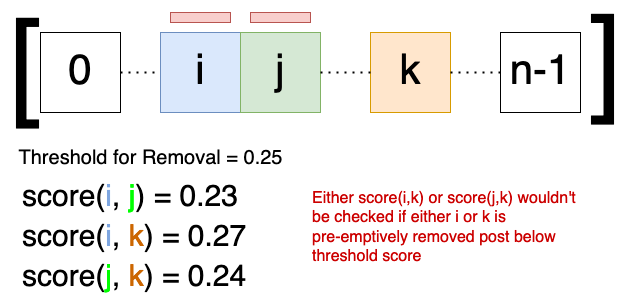
\includegraphics[width=0.6\linewidth]{diagrams/arraySimilarity.drawio.png}
    \caption{Example showing how a similar entry in the array may not be removed if earlier similar entries are removed pre-emptively}
    \label{fig:arraySimilarity}
\end{figure}

As demonstrated in \ref{fig:arraySimilarity}, to guarantee all duplicates are properly removed, as well as due to mapping hash map techniques being unable to be used, every entry must be checked against every other entry (with a higher index than it) in the array. Therefore, for an array of length $n$, we perform an average of $n \times \frac{n}{2}$ approximate string matching algorithm calls, giving our duplcate removal process a complexity of $O(n^2)$. To prevent concurrent access errors as well as to avoid pre-emptively removing a duplicate case, we implement this by creating a vector of boolean values of length $n$ (denoted as $B$), each defaulted to false. When we see a pair of indices in the array of entries which need removing with indices $\{i,j\}$ where $j > i$, we set
$B_j$ to true.

Once we have finished findings duplicates we simply iterate over our entry set and only return the entries where their associated index in $B$ is false.

The threshold value on the result of the Jensen-Shannon (JSD) metric between two strings was chosen through experimental analysis by using a combination of the like strings we have seen used for deciding on the algorithm of choice. The JSD metric is computed on both the author and title fields of each entry separately, then the average is computed of these scores. In the end I settled on 0.30 as the `duplicate' threshold. I found that this value very rarely falsely missed duplicate entries, and even more rarely cited two non-duplicates as duplicates.
% TODO: examine error rate of the algorithm?

\subsection{Compiling a Rust Library into a Node Module}
In order to make calls from our frontend GUI app to the rust code we produced, we need to provide some interface which can transform data types between the two languages. To do this we utilise the library \textit{neon} \citep{neon}. This provides a number of rust types and build modules to allow us to transfer the dynamically typed node Javascript variables into statically typed rust variables, it additionally builds our library file into a \code{.node} output which allows it to be required as a module in our Javascript code; hence allowing us to call our written functions. The code running is still compiled and builds rust binaries, as such there is no loss of speed besides the overhead on type conversions.

To perform the conversions, Neon provides the \code{FunctionContext} object which provides ``a view of the JS engine in the context of a function call", hence giving us access to things like function arguments. Using this objects \code{argument::<T>(index)} method allows us to access each object in the array of arguments, as well as specifying a type, \code{T} - allowing us to do type checking on the arguments we receive!

Converting types back into valid Javascript types is equally smooth with Neon; the \code{FunctionContext} object also can be used to convert standard types into their relevant JS type. JS objects can also be created and their keys set with a value pair; allowing us to convert structs into similarly shaped JS objects. The code for converting our BibEntry type into its JS Equivalent can be seen in figure \ref{fig:bibEntryConversion}.

\begin{figure}
    \begin{minted}{rust}
    fn to_object<'a>(&self, cx: &mut FunctionContext<'a>) -> JsResult<'a, JsObject> {
        let obj = cx.empty_object();

        let entry_type = cx.string(self.entry_type.clone());
        obj.set(cx, "entryType", entry_type)?;

        let name = cx.string(self.name.clone());
        obj.set(cx, "name", name)?;

        let fields = JsArray::new(cx, self.fields.len() as u32);
        for (i, field) in self.fields.iter().enumerate() {
            let field_obj = field.to_object(cx)?;
            fields.set(cx, i as u32, field_obj)?;
        }

        obj.set(cx, "fields", fields)?;

        Ok(obj)
    }
    \end{minted}
    \caption{Converting our BibEntry struct into a similarly structured JS object with neon.}
    \label{fig:bibEntryConversion}
\end{figure}

As a result of all of the above writing rust code to be ran as a node module is surprisingly simple, this allows us to utilise the power of rust within our application. Although not used as of yet a future goal for the project could be to utilise rust's concurrency race safety guarantees to parallelise the operations we perform, hence speeding up our application even more.

\subsection{The GUI}
The goals of the GUI have already been laid out in earlier sections; to create an easy to use, responsive and simple UI; to allow the user to access all the functionality we have worked hard to achieve!

To aid in the development of the GUI we utilise a number of technologies to help us more effectively and efficiently build our application. Luckily, due to Electron, our desktop application framework of choice, we gain access to all frontend and web technologies which are node modules. This list is extremely extensive inclduing frameworks such as VueJs, Angular, Svelte and more, as well as a long list of styling frameworks and component sets. For this project I chose to use typescript with react as a framework, using Material UI \cite{mui} to style our components.
\subsubsection{Electron, React}
Building our application in electron allows our app to be cross platform by default. It allows us to use Javascript, HTML and CSS to easily build pretty and usable GUIs quickly with the high level abstractions they provide over rendering. Using react on top of this allows us to compartmentalise our application into components. These are re-usable making separating our app and keeping our codebase in order easy to do. Typescript on top of this ensures type safety between components and function calls; this is evermore important in our context due to the type-constrained rust module functions we will be later calling in our application. As well as this guaranteeing type safety prior to runtime can help identify type based errors before they occur; preventing some unforeseen bugs.

We will discuss the layout of the GUI as well as specific UI choices more later in the section \textit{GUI Design}, however to aid in this we use the component library `MUI" \cite{mui}. This provides pre-built React components where styling and functionality can be customised through the passing of props. It also provides additional functionality such as easy app-wide theming. I chose to use this component library as it allowed me to make my GUI act and appear as I hoped for it to appear, whilst saving me time performing busy work creating my own components. This work would not have been within the main goal of the application and as such would have distracted from the work done on the underlying logic behind the application. 
% react-electron boilerplate, typescript
\subsubsection{Native Modules in Electron}
Native modules define any node dependencies which are written in an external language such as rust. Hence, the Neon module we have built can be defined as a native module in the context of this application. For building my application I am using an NPM boilerplate library known as electron-react-boilerplate \cite{electronReactBoilerPlate} which utilises other npm packages such as webpack to bundle and build modules. Native modules, to quote the documentation, ``can be problmeatic" when bundled with webpack, and as a result are treated as webpack externals.

Webpack external rely on the dependency being referenced to be present in the end-user-applications environment, hence they are bundled with the application when creating a production deployment. Doing this allows root dependencies (such as react in our case) to not be packaged with the app once it is built; reducing app bloat \cite{electronReactBoilerPlate}. In order to bundle a native application as a webpack extneral we instead install our native dependency to \code{./release/app/node\textunderscore modules} rather than \code{./node\textunderscore modules}.

Native modules can be quite difficult to manage and import in an electron app. This is because the electron app runs in two (main) separate threads; the main process and the renderer process. The main process is running natively and building the application windows that are shown to the user, it is also interacting with environment/OS processes. Hence it is able to make lower level system calls and thus is better suited to dealing with calls such as our calls to our native library (as well as other features we need such as interacting with the local file system). In contrast the renderer process(es) simply have control of each window spun up by the main thread. Its main responsibility, surprisingly, is \textit{rendering} web content. As a result this is not the best suited environment for performing lower level; OS level function calls. As a result electron disables loading remote content in the renderer process by default as it is considered a security vulnerability.

Because of this, we now have some \textit{context isolation} between our main thread and our renderer threads; there are operations performable in the main thread unavailable in the renderer thread which we will wish to access; such as loading BibTeX file data using our library and displaying it to the user. To do this, we can use a \code{ContextBridge} defined in a preload script to share an interface between the two processes. This allows us to perform inter-process communication (IPC) to trigger main process tasks from our renderer (this also allows vice-versa, but this is not needed).

\subsubsection{IPC Calls}
As described above, IPC calls allow our renderer process to make calls across to the main thread to perform processes locally, which can then return the information. To do this we create a preload script which creates a context bridge, and exposes an API to the ``main world"; I.E. our renderer process.

Our API is an instance of the ipcRenderer electron object. Using this object in our renderer process we can call the \code{ipcRenderer.send(channel, args)} function to send a set of arguments down a given channel. Back in our main process we can then create channel listeners, who on receiving a request from than channel, can process the arguments, perform some function and return the results back down the same (or different) channel. See figure \ref{fig:ipcCalls} for a diagram of this.

\begin{figure}
    \centering
    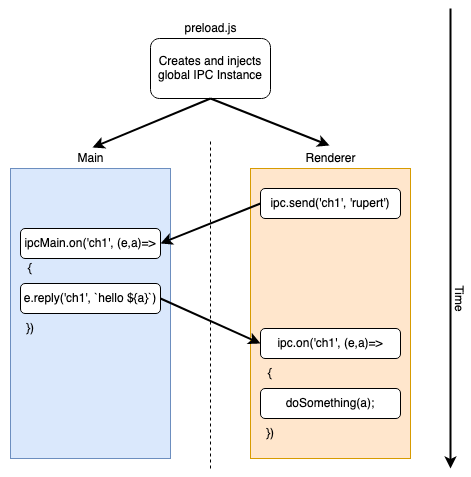
\includegraphics[width=0.6\linewidth]{diagrams/ipcCalls.drawio.png}
    \caption{Inter Process Communication call structure in electron}
    \label{fig:ipcCalls}
\end{figure}

We use this process to make our calls from the renderer process to the main process to access our created functions in our native module. A benefit of IPC calls in electron and react is that the calls are non-blocking (asynchronous), as a result more expensive operations such as parsing all the files retrieved, or merging a large number of files can be performed without interrupting the renderer process. This allows the status of operations to be shown to the user whilst allowing them to still interact with the rest of the application.

An example of this in use is after a user has searched for a returned a number of files on their disk. The application will immediately display the results of the search to the user. Each of these files then needs to be parsed in order to display to the user information about each file; if we were to do this synchronously then the application would be frozen until each of the possibly hundreds of files had been parsed. Instead the asynchronous calls means that this information can be loaded in as each file's processing is completed, preventing the user from experiencing this delay.

\subsubsection{GUI Design}
When designing the UI, to maintain the goals I have already laid out, I wanted the layout to be minimalist; presenting as little as possible to the user whilst simultaneously presenting all the information that it is important or useful for them to see. Additionally, due to the nature of this application the user may be dealing with thousands of pieces of data; to display all of these to the user at once would be overwhelming and degrade the overall experience. Hence this is also something to avoid.

The immediate page the user is presented is the Homepage. On each page of our application there is consistently a navbar menu which can be toggled to be able to access the different pages on offer to the user. This being togglable allows the user to only view it when they wish to use it, preventing it from cluttering the rest of the information on screen. This NavBar can be seen in figure \ref{fig:navbarScreenshot}. The NavBar is dynamic and is designed to only be on screen for the minimum amount of time as needed; meaning it automatically closes when elsewhere is clicked, or if a link is used.

\begin{figure}
    \centering
    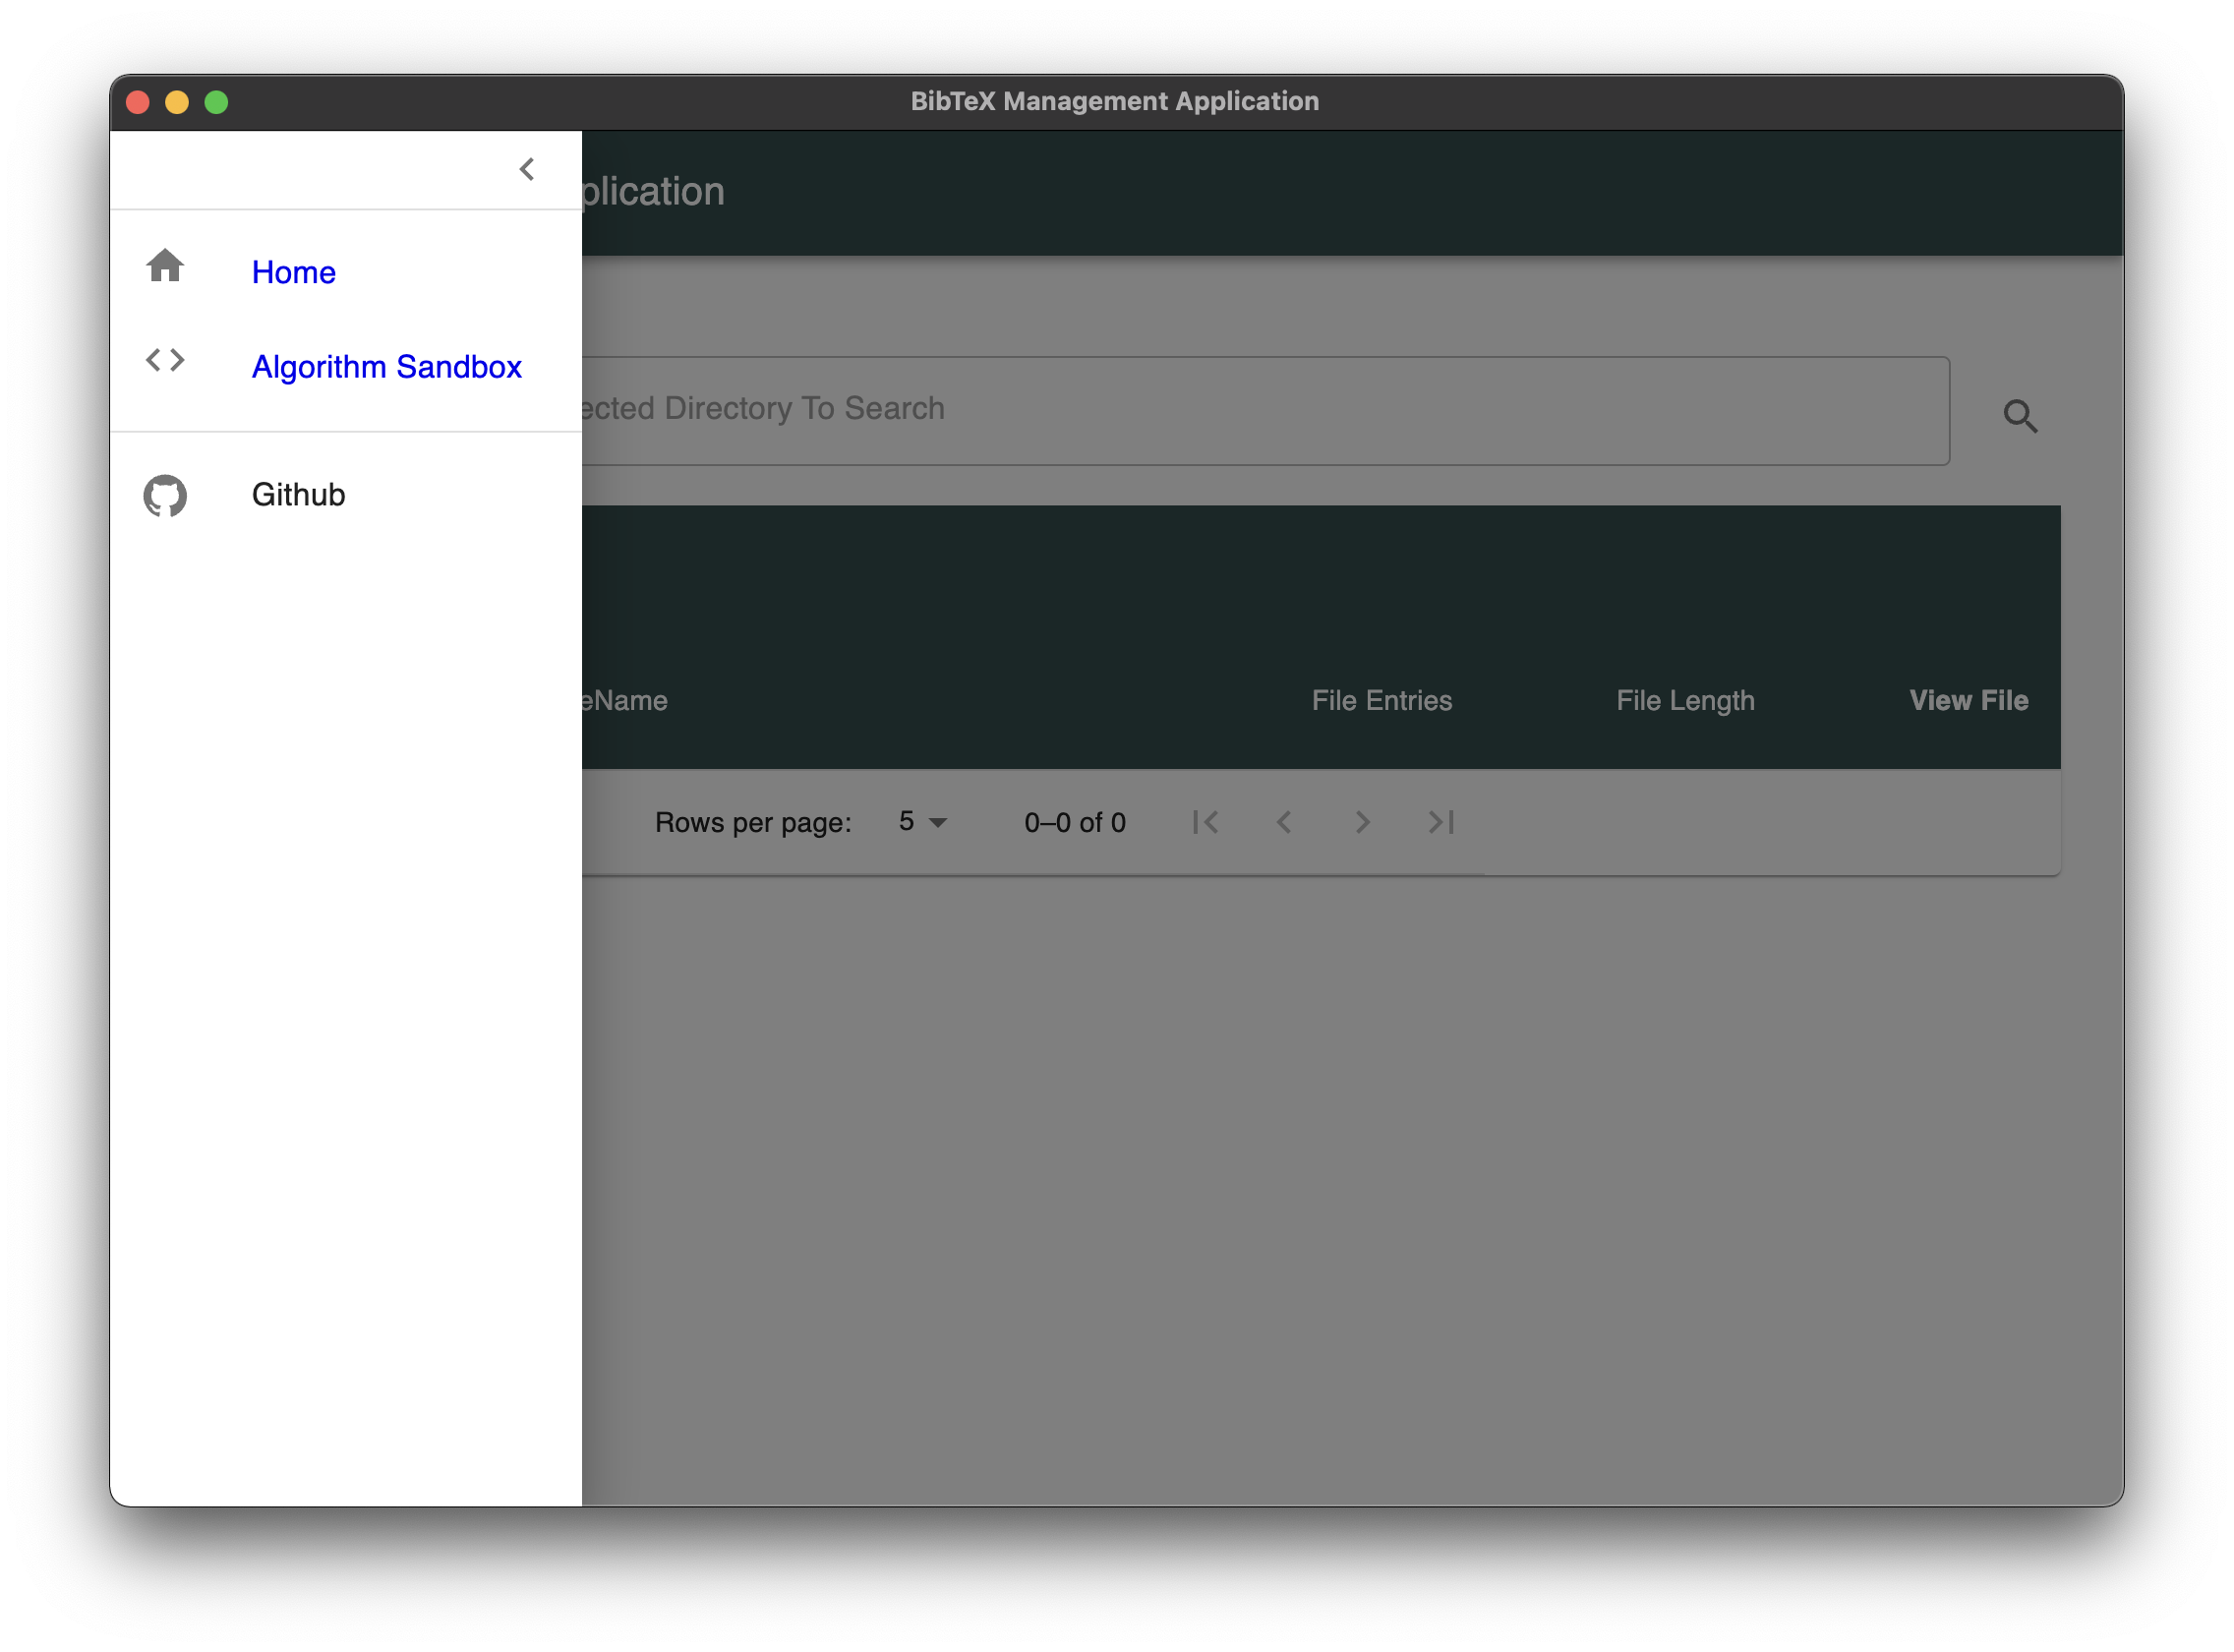
\includegraphics[width=0.8\linewidth]{images/navbar.png}
    \caption{Screenshot of the Navbar on the GUI of this application}
    \label{fig:navbarScreenshot}
\end{figure}

The Homepage provides access to the main functionality of the application. This is where the user can search a volume for a file, see all the files it returns, select the files they want to merge and then merge the files.

Each of these pieces of functionality have distinct areas of the homepage which they are designated to.

At the top of the page is the area for selecting a local directory and searching it in order to find files with the \code{.bib} extension (this can be seen in action in figure \ref{fig:fileSelectionToSearch}). The directory search makes use of the local file system explorer, therefore making the code agnostic to whatever environment it may be operating on. The user will also be familiar with this system and thus it lowers onboarding time as the user does not have to learn a new file system GUI.

\begin{figure}
    \centering
    \begin{subfigure}{0.49\textwidth}
       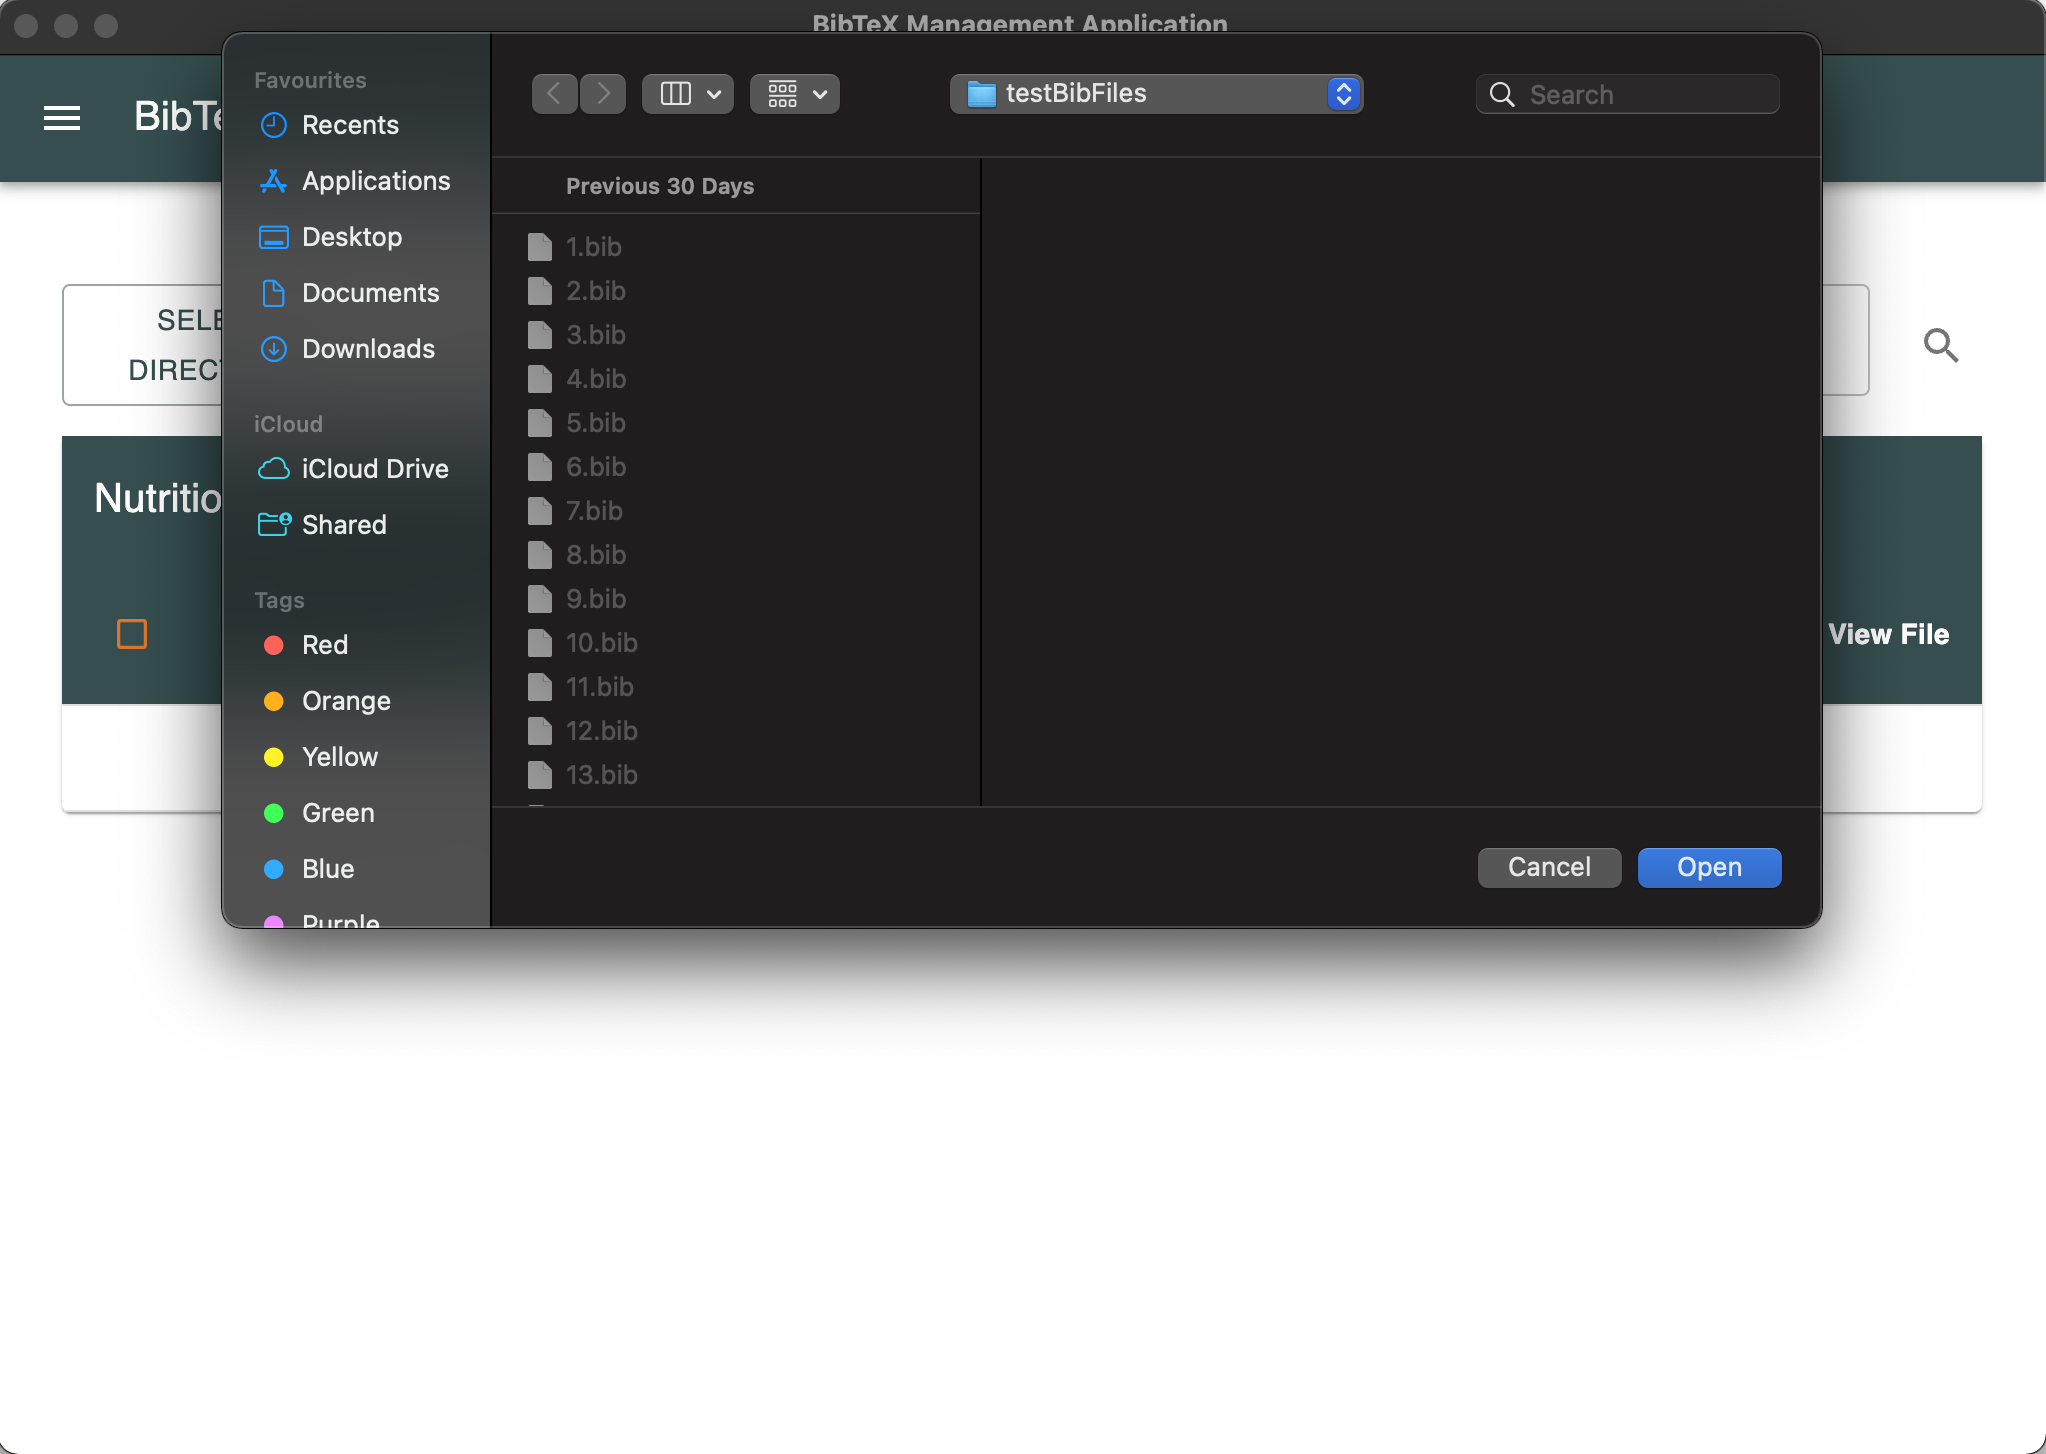
\includegraphics[width=\textwidth]{images/selectingFileSearch.png}
    \end{subfigure}
    \begin{subfigure}{0.49\textwidth}
       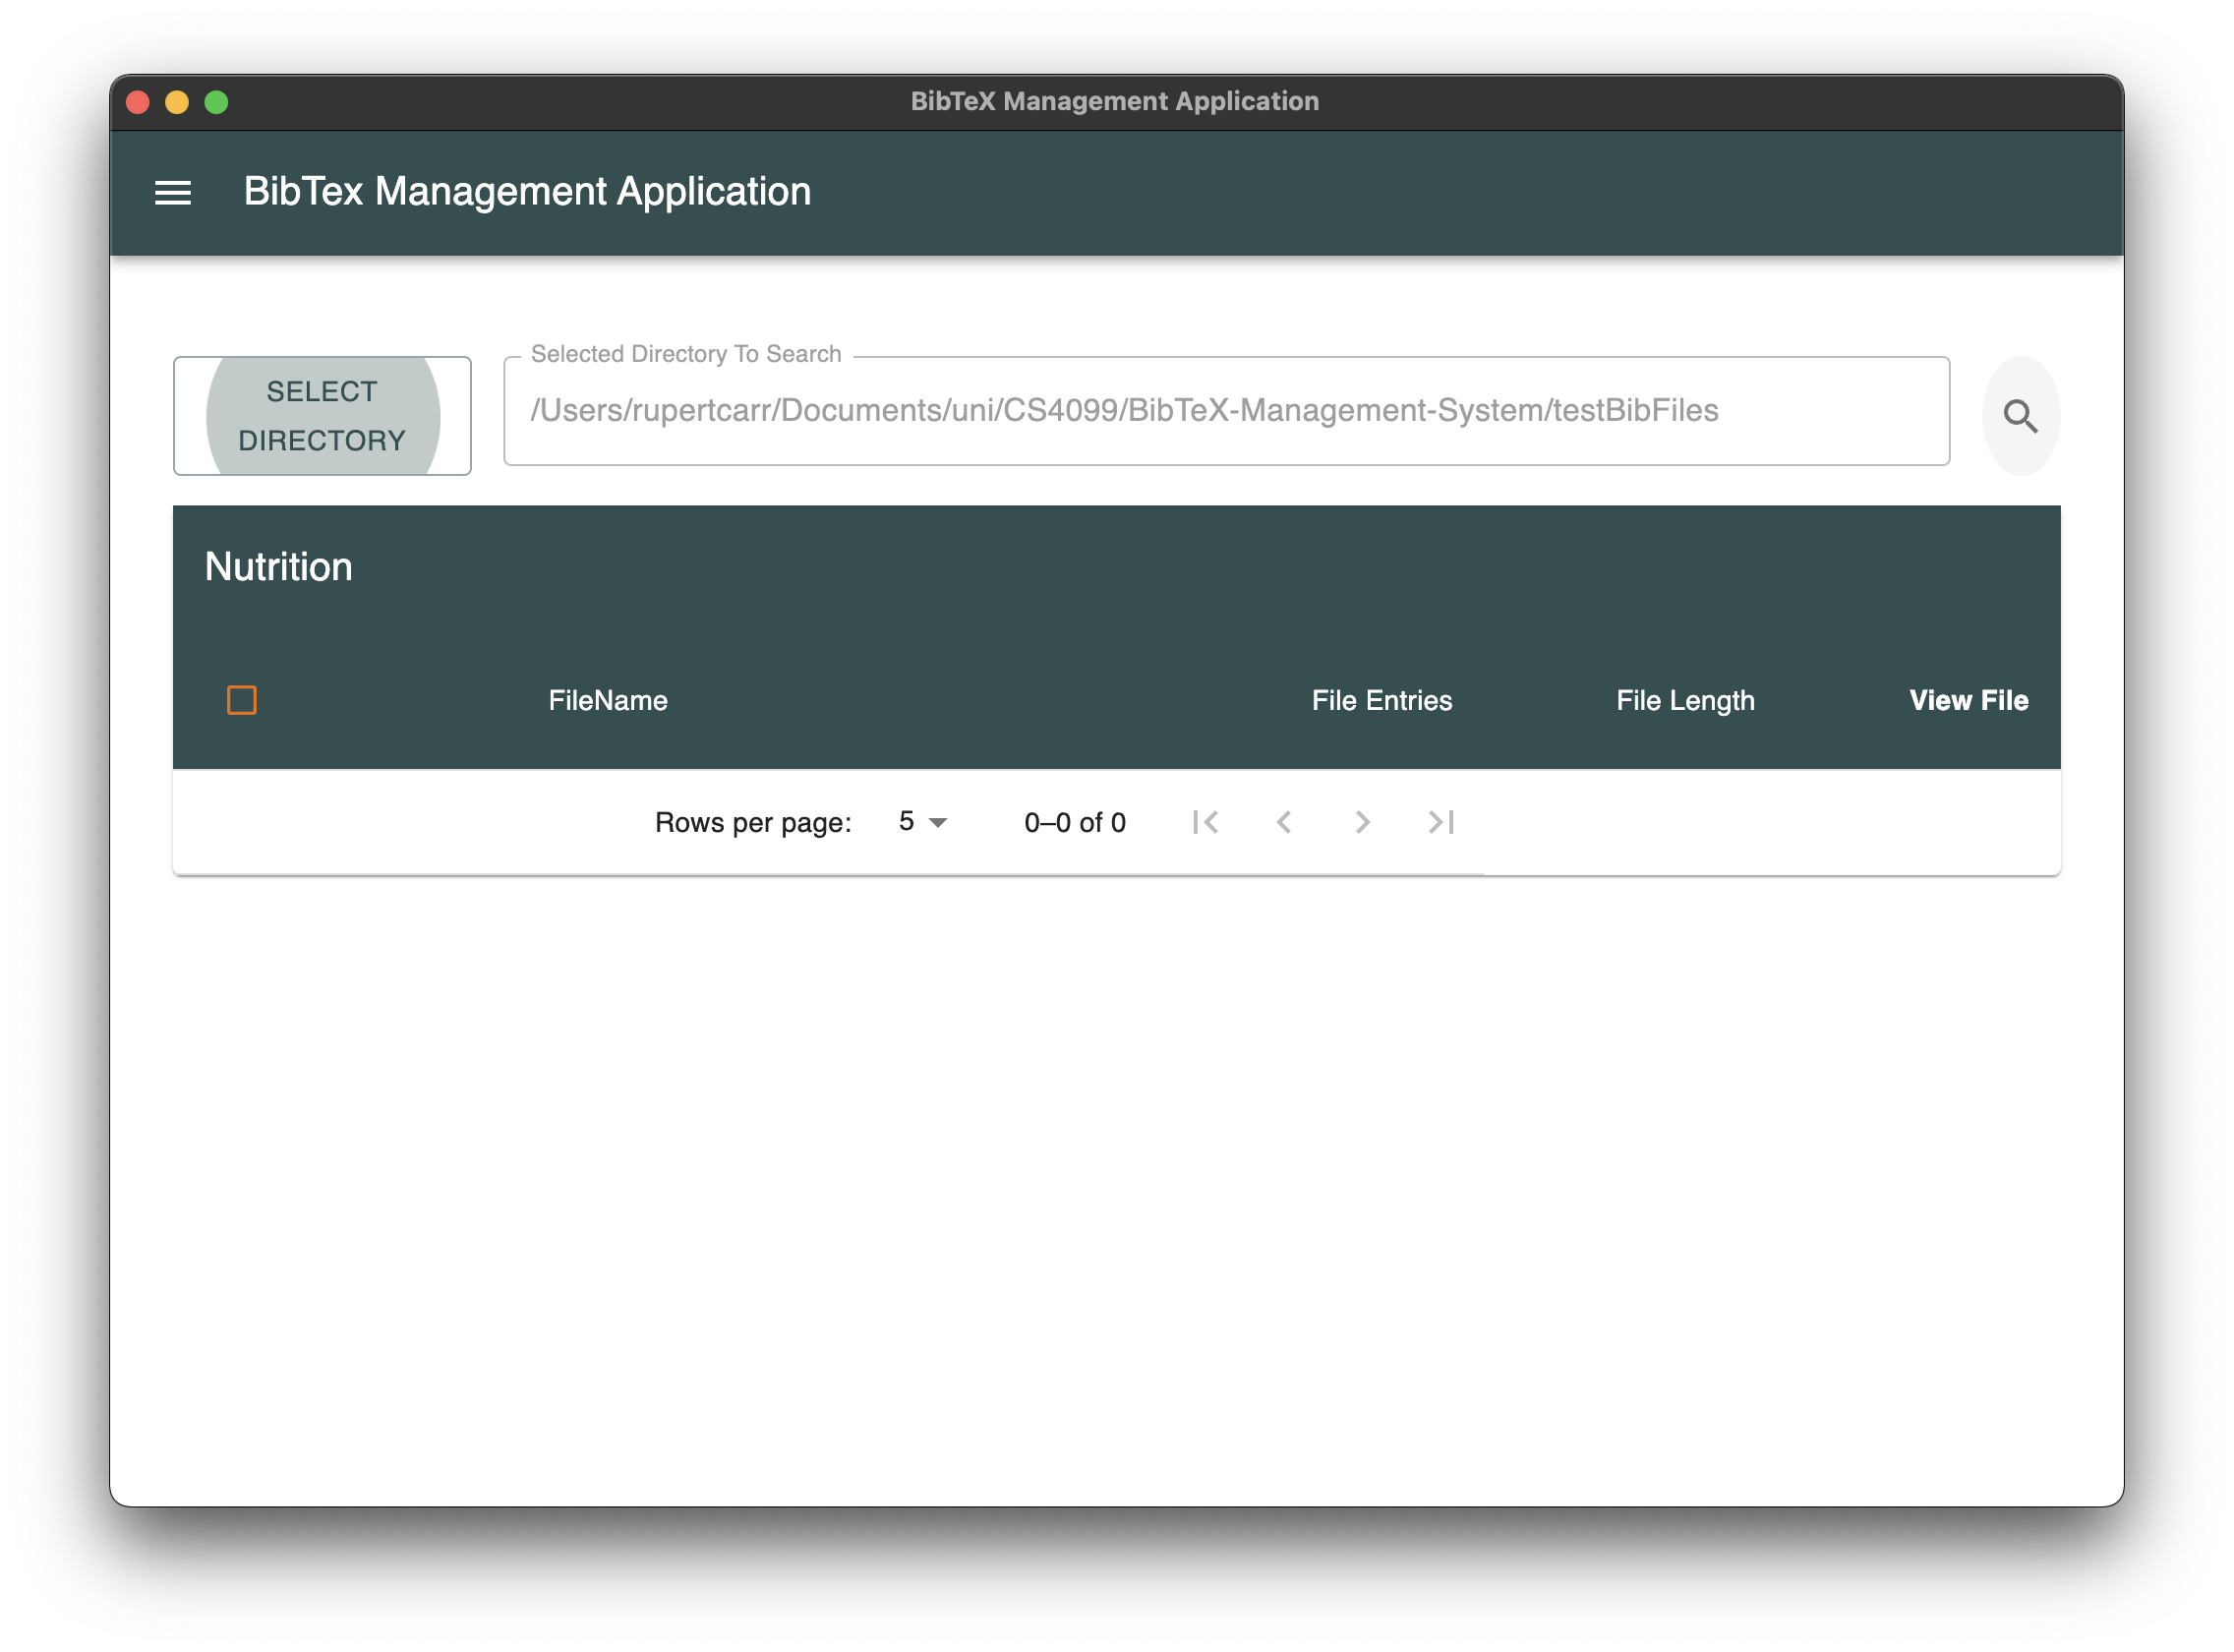
\includegraphics[width=\textwidth]{images/fileSelectedToSearch.png}
    \end{subfigure}
    \caption{Selection and selection result when choosing a directory to search for BibTeX files on the GUI}
    \label{fig:fileSelectionToSearch}
\end{figure}

Once the user has searched for the files, we don't want to overload the user with information. Hence I decided a table display, along with pagination would be the best way to display information to the user without overwhelming them, but yet give them easy access to navigate through the files and select those that they wish to use and merge. This is done with the aid of MUI's \cite{mui} table component, which provides somewhat easy to use pagination methods to break up the long array of rows into separable slices/pages.

By default the user is shown groups of five files on each page, although this can be adjusted through a drop down on the bottom. Which files are currently being shown (for example ``20-24 of 53") is displayed to the user such that they have track of where in the result set they currently are. Navigation buttons are also provided with commonly known icons to symbolise them; meaning that most users will easily instantly recognise their function and use. See figure \ref{fig:pagination} for pagination example.

\begin{figure}
    \centering
    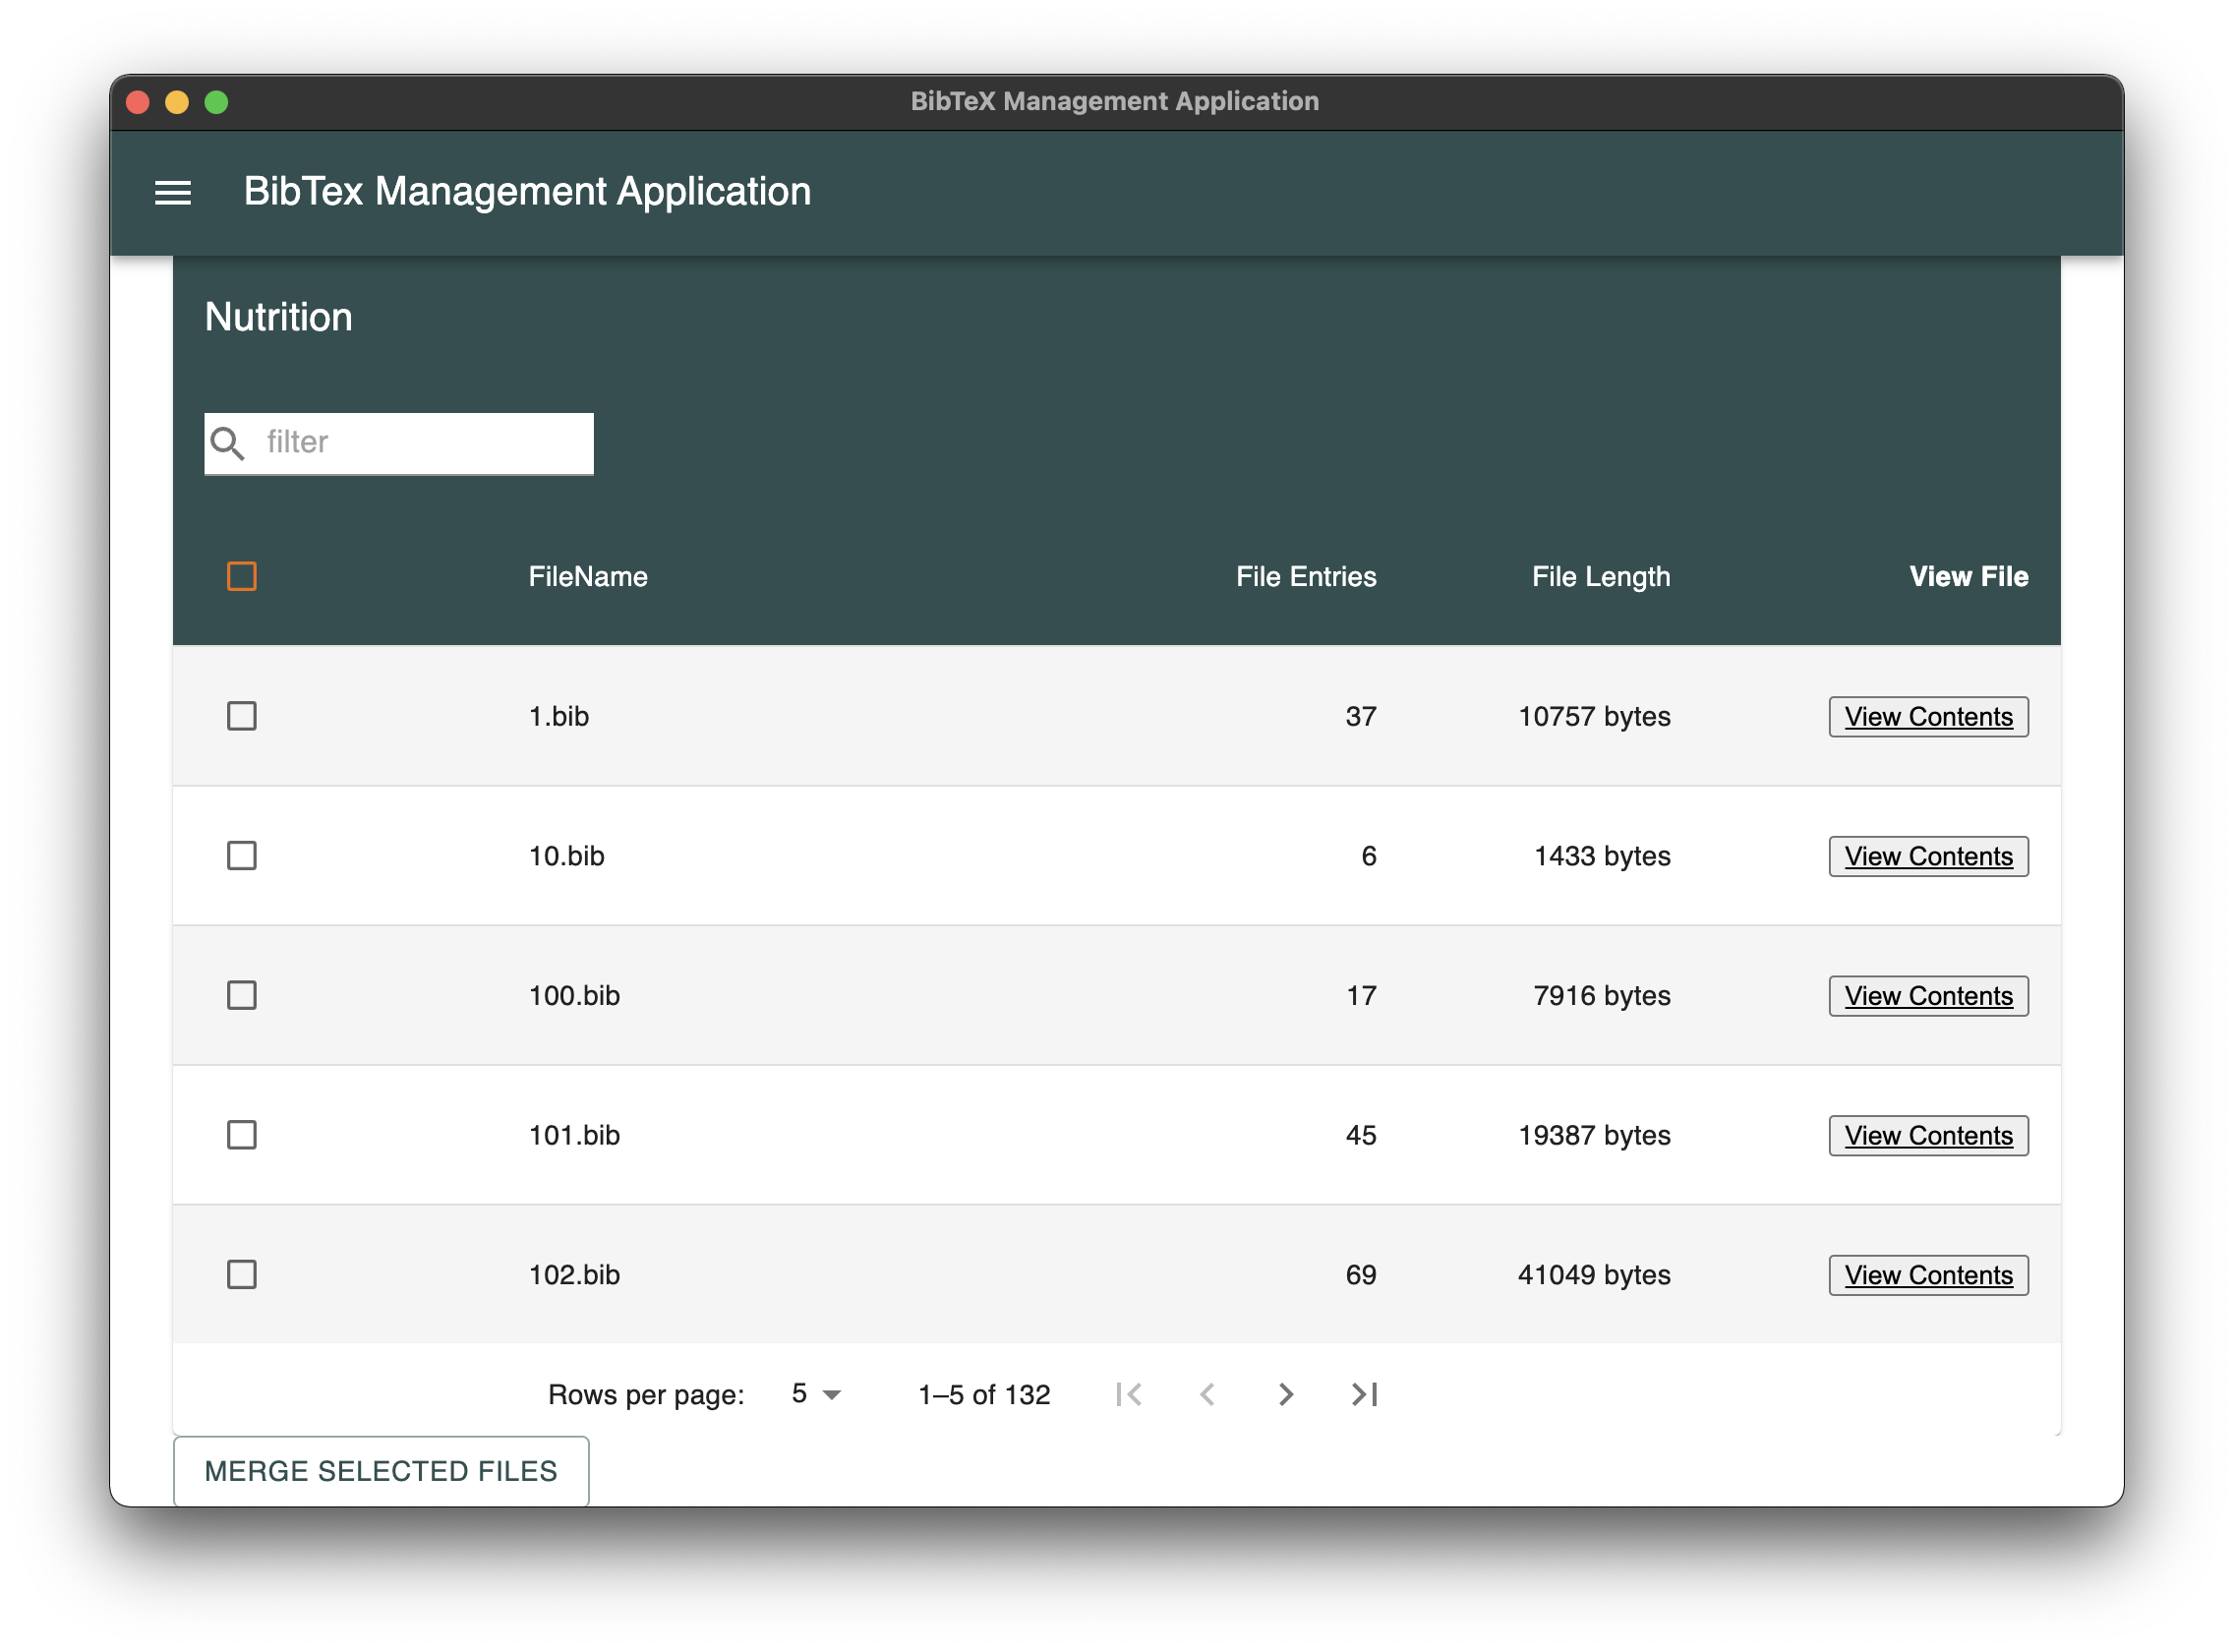
\includegraphics[width=0.8\linewidth]{images/pagination.png}
    \caption{Pagination of search results in the GUI}
    \label{fig:pagination}
\end{figure}

Additionally to pagination a filter function has also been implemented. This allows a user to directly search and filter for a file name. Particularly if the user has come up with results for many bib files within a volume, if there are particular files they wish to use they should not be subject to paging through all the results, accessing the files they want to merge should be as easy as possible. The filter function aids in this. The filter function currently just uses the built in \code{string.includes(arg)} function to filter down the list of results, but given more time this could be extended to again make use of our approximate string matching algorithms!

In each row of the file the following information is displayed to the user.
\begin{itemize}
    \item The file name
    \item The number of entries in that file (successfully parsed)
    \item The file size (in bytes)
\end{itemize}
The information provided here aims to aid the user in finding the files they want to see. This information is gathered internally by parsing the file to gather the entries.

To further help the user identify the files they wish to parse, the user can also click the `view contents' button. This brings them to a page containing a table with each row representing one parsed entry of the file. Each of these rows displays the following (this can be seen in figure \ref{fig:fileEntries}).

\begin{figure}
    \centering
    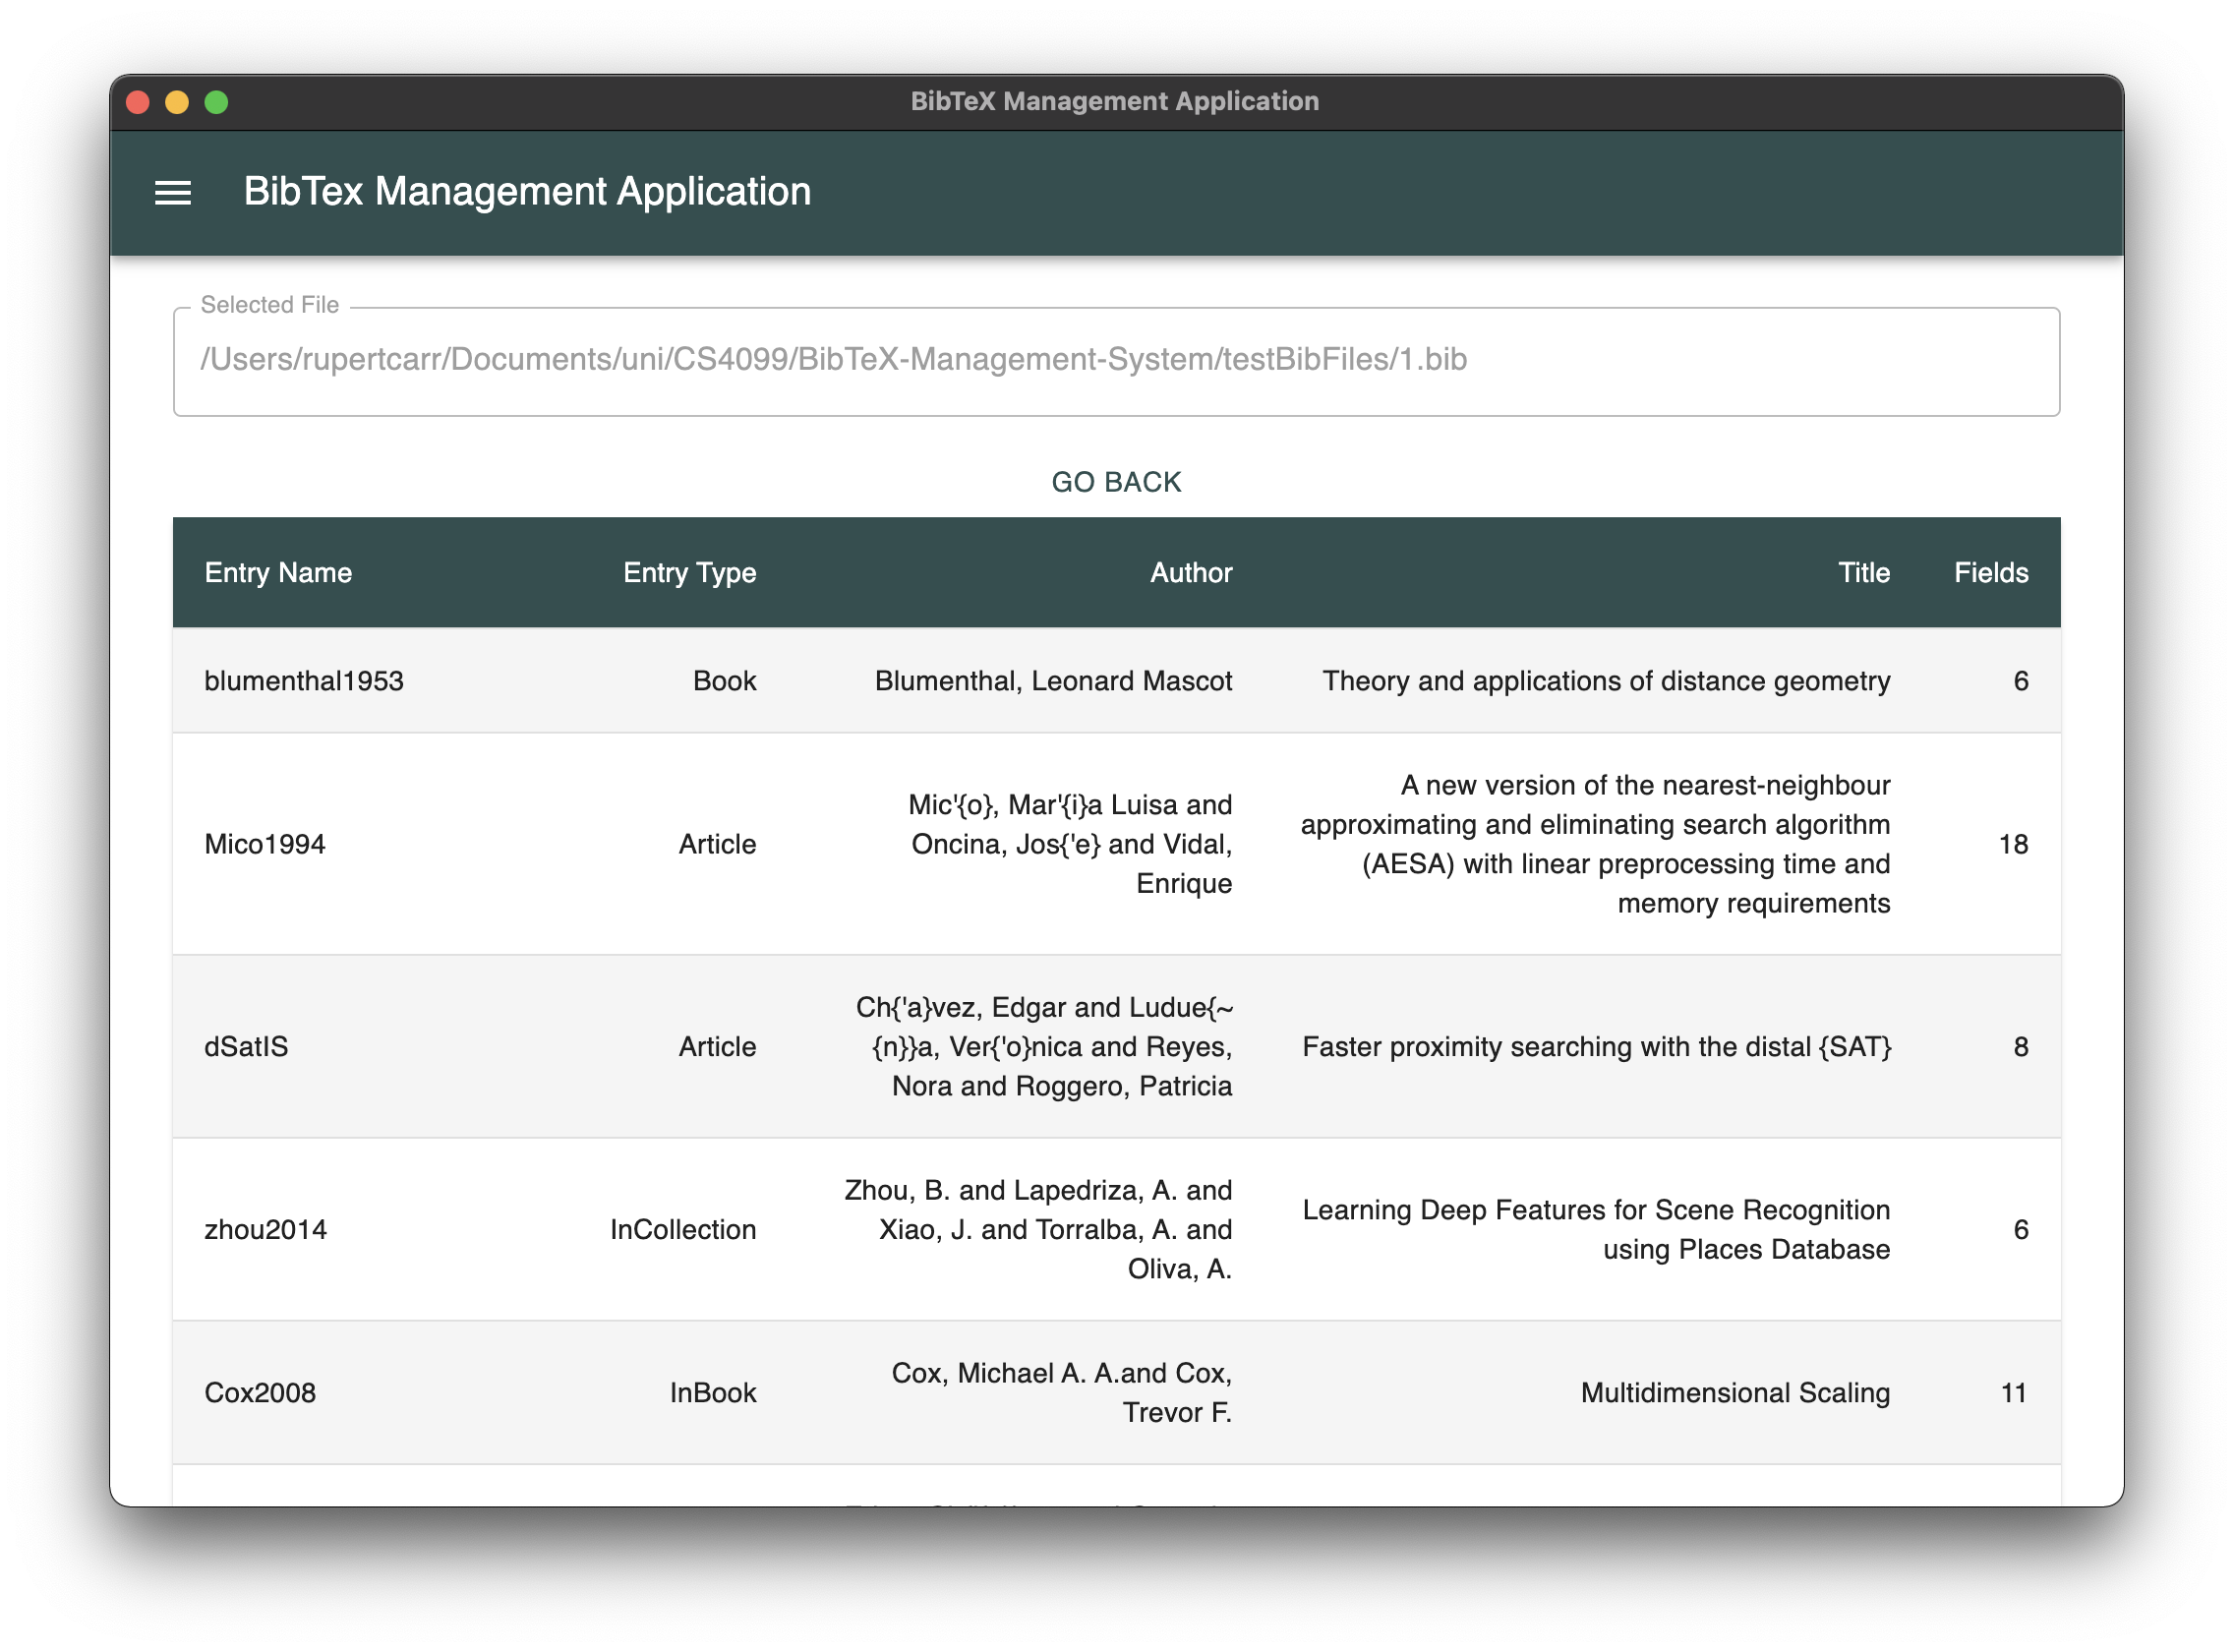
\includegraphics[width=0.8\linewidth]{images/fileEntries.png}
    \caption{Page showing in table format the parsed entries within a file}
    \label{fig:fileEntries}
\end{figure}

\begin{itemize}
    \item Entry Name (citation key)
    \item Entry Type
    \item Author
    \item Title
    \item Fields (number of)
\end{itemize}
The user can then click on any entry, and a modal will be displayed to them showing the rest of the fields in that entry and their respective values, see figure \ref{fig:entryContents} for this in action.

Once again, the goal of this is to allow the user to view their files and their content within the application, allowing them to better identify which files they wish to merge; without the need to exit or tab out of the application. This enhances user experience.

\begin{figure}
    \centering
    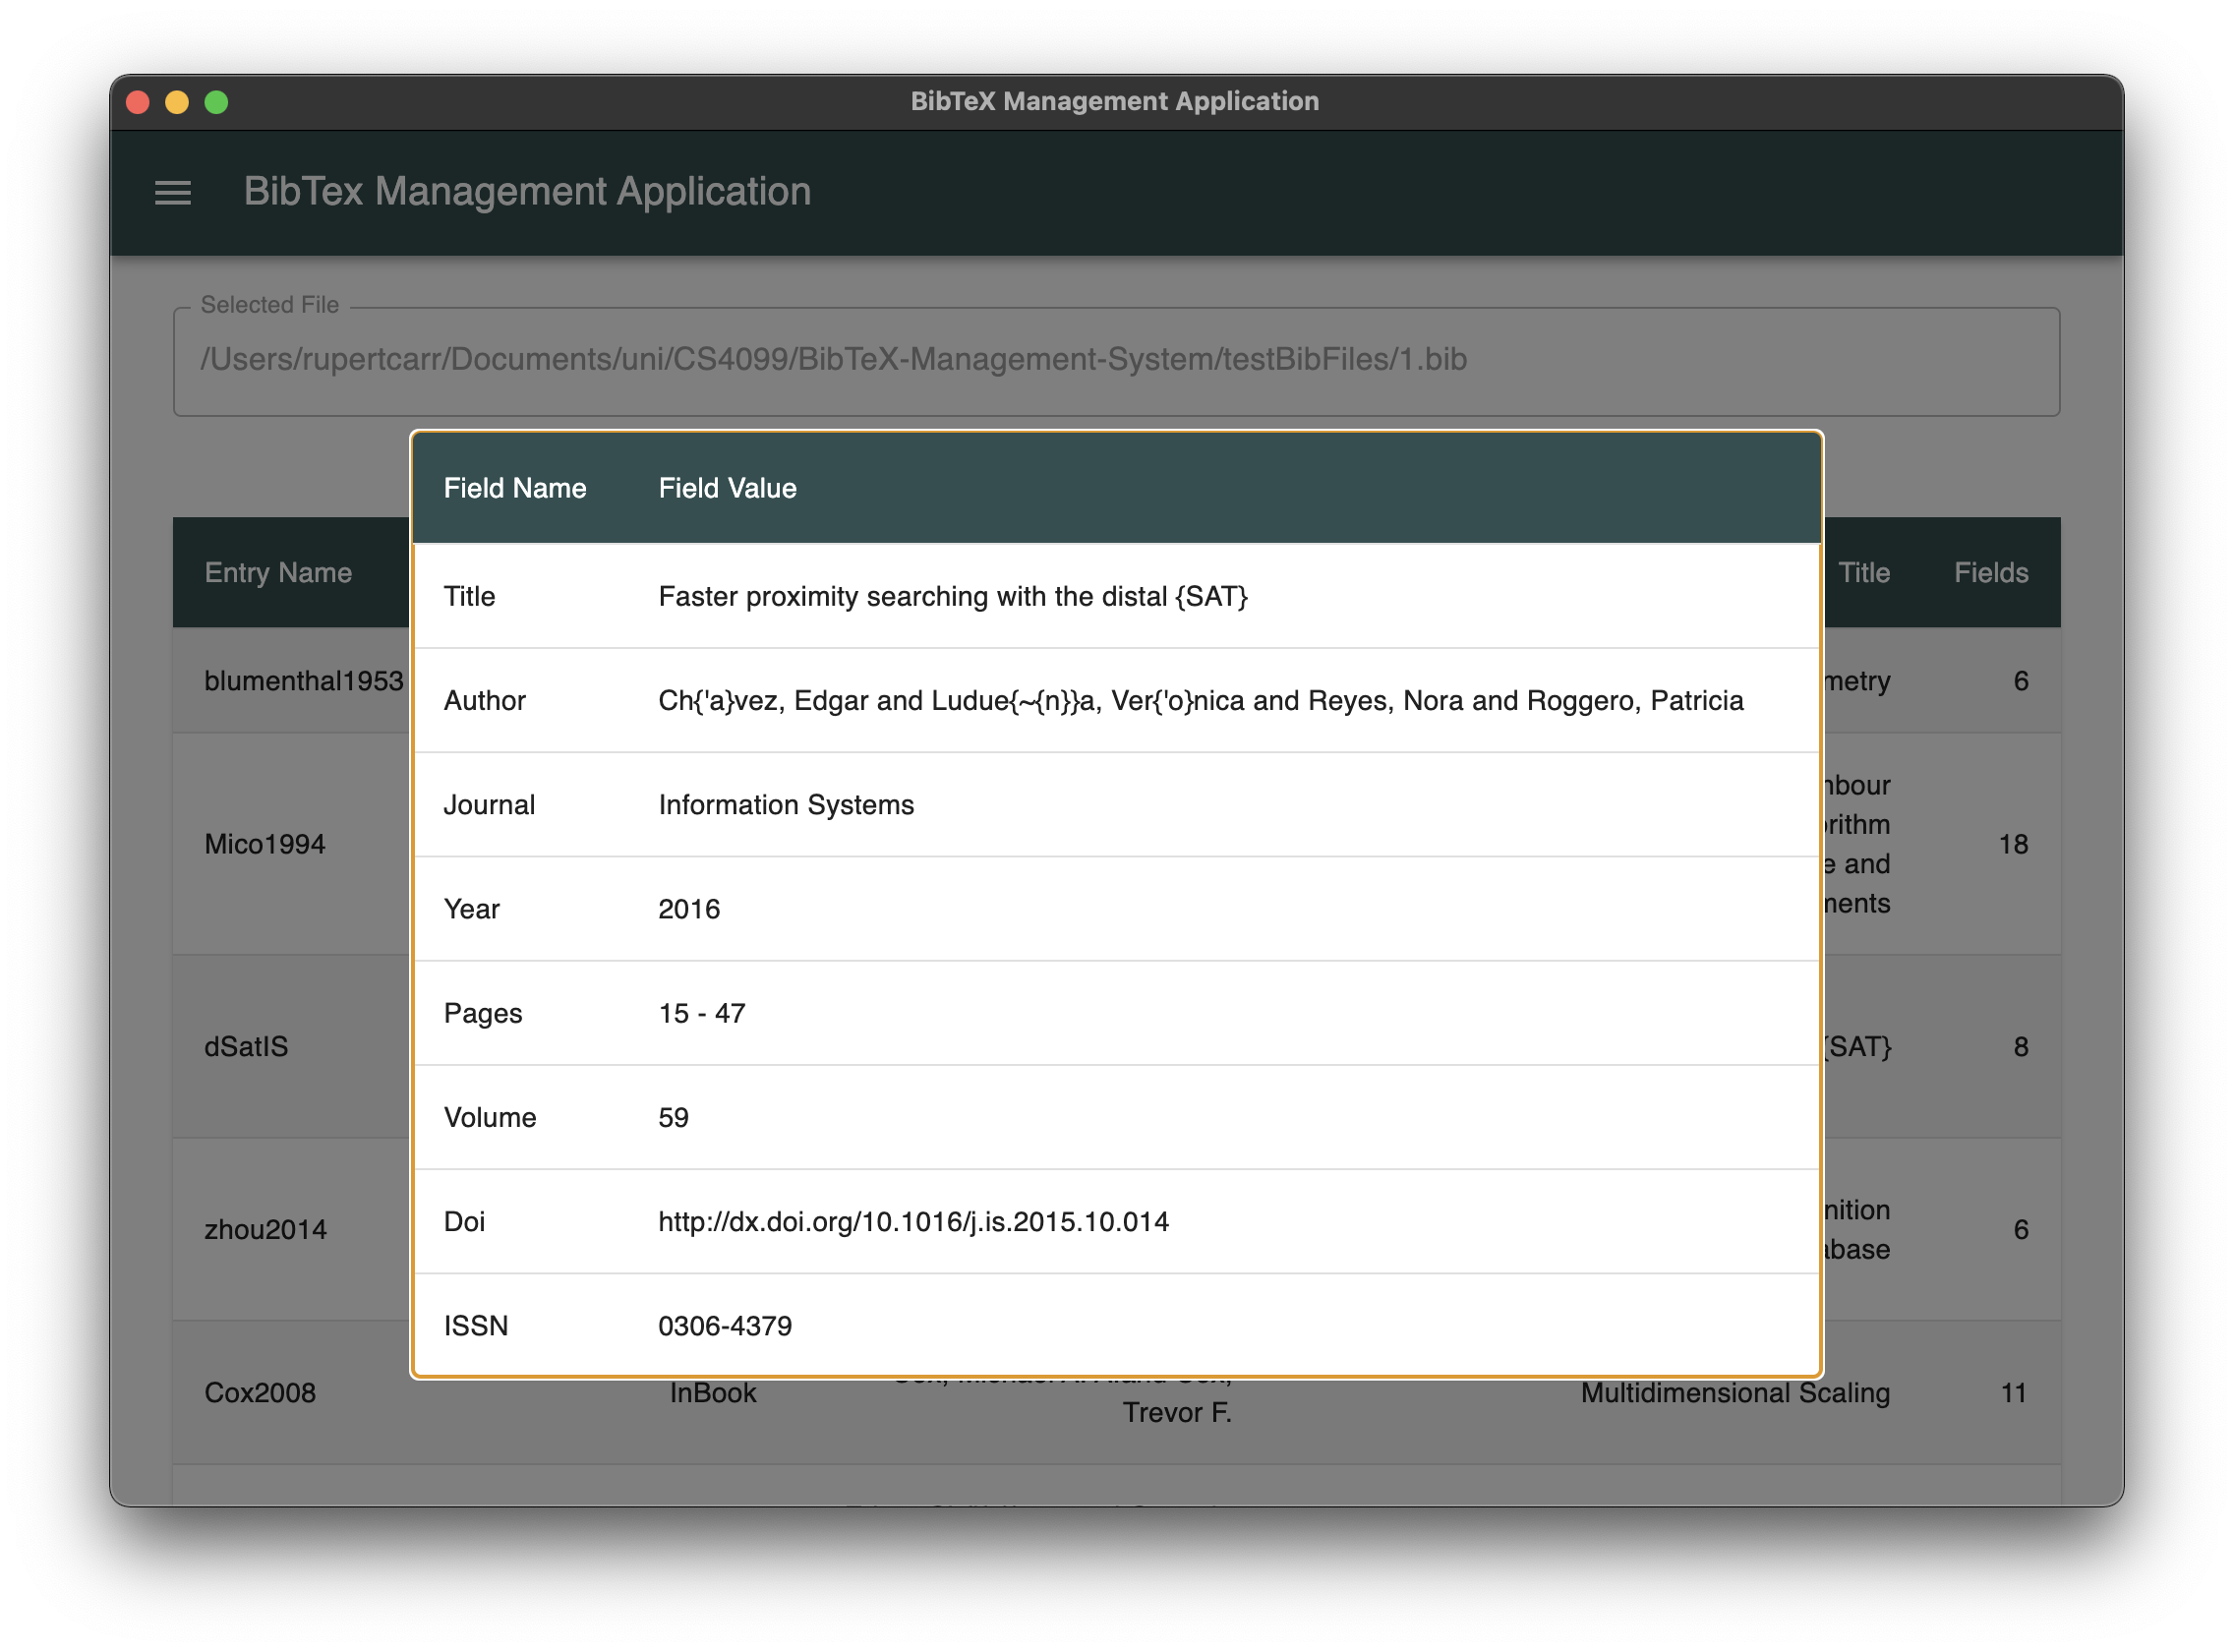
\includegraphics[width=0.8\linewidth]{images/entryContents.png}
    \caption{Modal displays more information about a given entry within a file when clicked}
    \label{fig:entryContents}
\end{figure}

A user can easily select a file that they wish to merge by clicking on that row, the status that a file is 'checked' to be merged can both be seen by a now checked checkbox on the left side of that row, as well as by a count of the number of selected files that the user currently wishes to merge. Additionally, before merging these files those that have been selected are displayed once again to the user in the merge modal.

All of this is important as the user is constantly given a clear indication of which files are selected, hence they are always feeling in control of what they wish to do within the application. Maintaining visibility and status to the user is crucial when creating an easy to use GUI.

On top of this, when files are selected a 'bin' icon is displayed to the user; when clicked this will remove all currently selected files from the list of selected files, allowing the user to easily remove their chosen selection if they so wish. All of this functionality can be seen in figure \ref{fig:selection}.

\begin{figure}
    \centering
    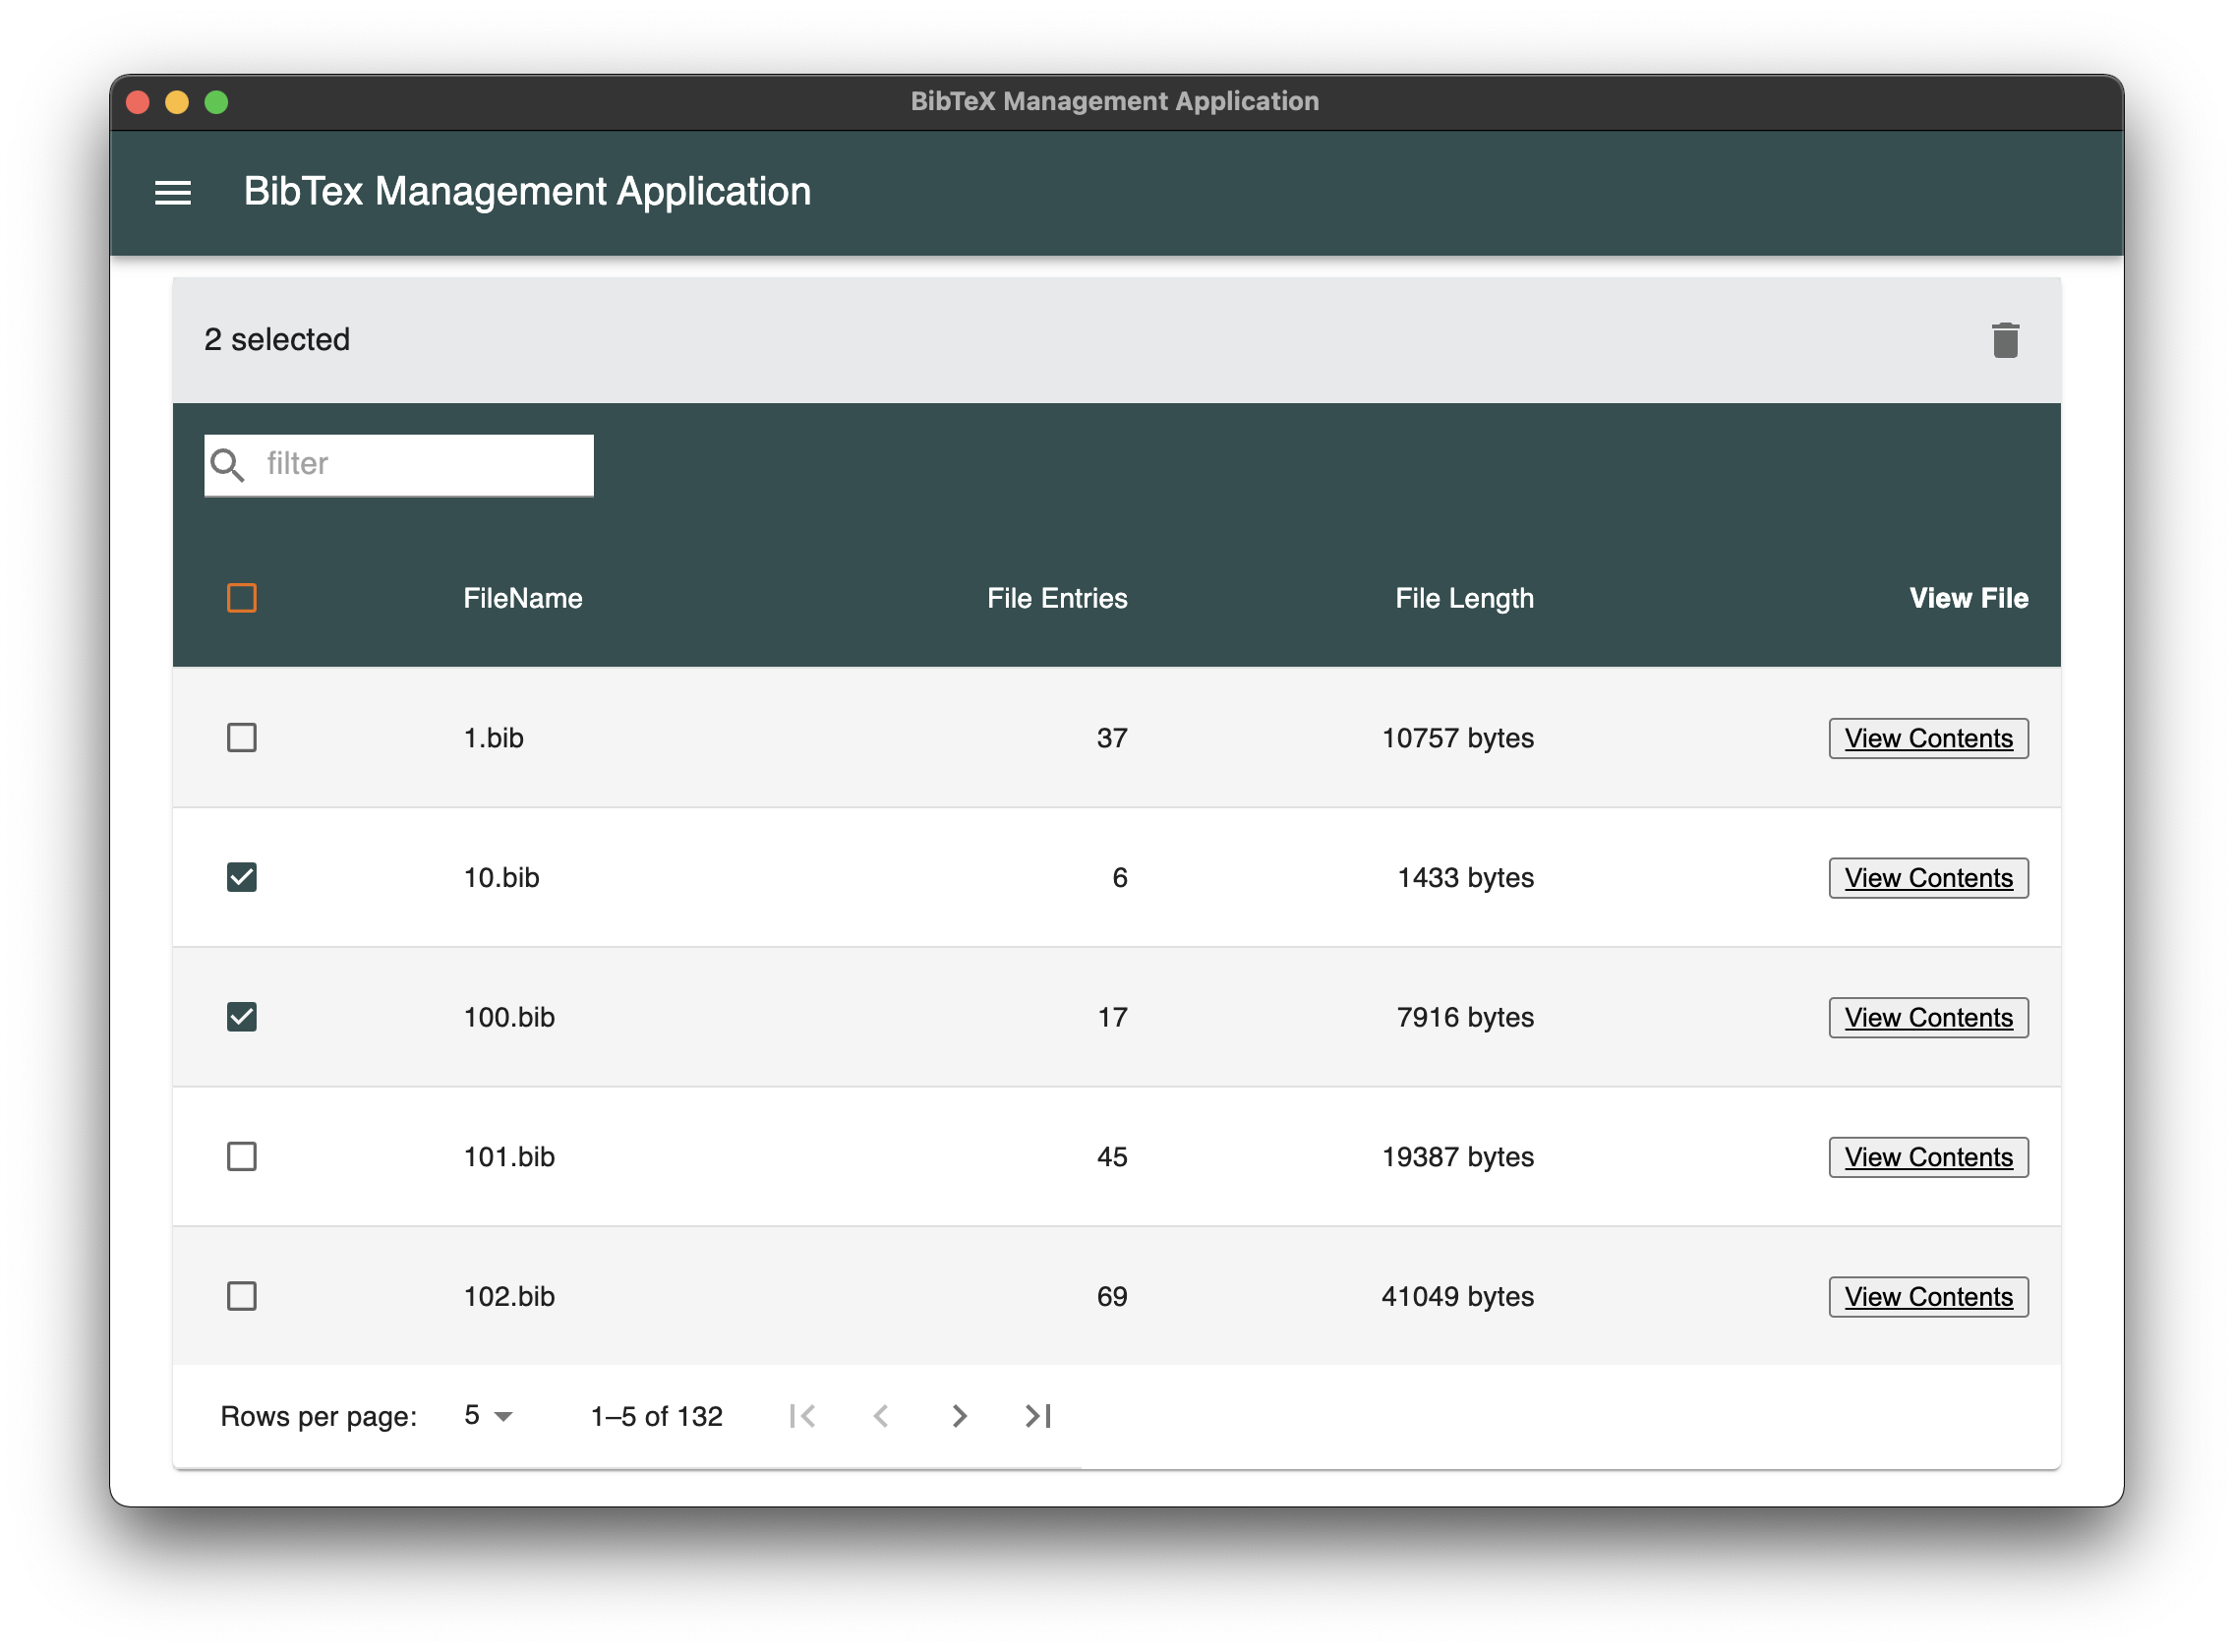
\includegraphics[width=0.8\linewidth]{images/selection.png}
    \caption{Number of selected files, as well as option to remove them, are displayed to the user.}
    \label{fig:selection}
\end{figure}

When a user is ready to merge their selected files, they click the ``Merge Selected Files" button at the bottom of the page. This opens a modal which displays necessary information to the user in order to complete this operation. This is also where the user chooses their output location for the merged files. Once again this utilises the local OS's file explorer, presenting the user with an interface that they are familiar with, decreasing onboarding time for the application.

Once again, status is maintained and shown to the user in this modal; both the selected files which shall be merged as well as the output location are both displayed to the user.

Once merged is click, the button icons switch to a ``loading" state, which only completes once the merge operation is finished. This again is an example of displaying status to the user; ensuring that they know that a merge is in progress in the background. An extension to this for future development would be to include some progress bar to increase the information shown to the user. Particularly for the larger merge operations over 10s or hundreds of files which may take a reasonable amount of time, this progress bar could let the user gauge progress more effectively. This modal, in its merge-loading state can be seen in figure \ref{fig:mergingFiles}.

\begin{figure}
    \centering
    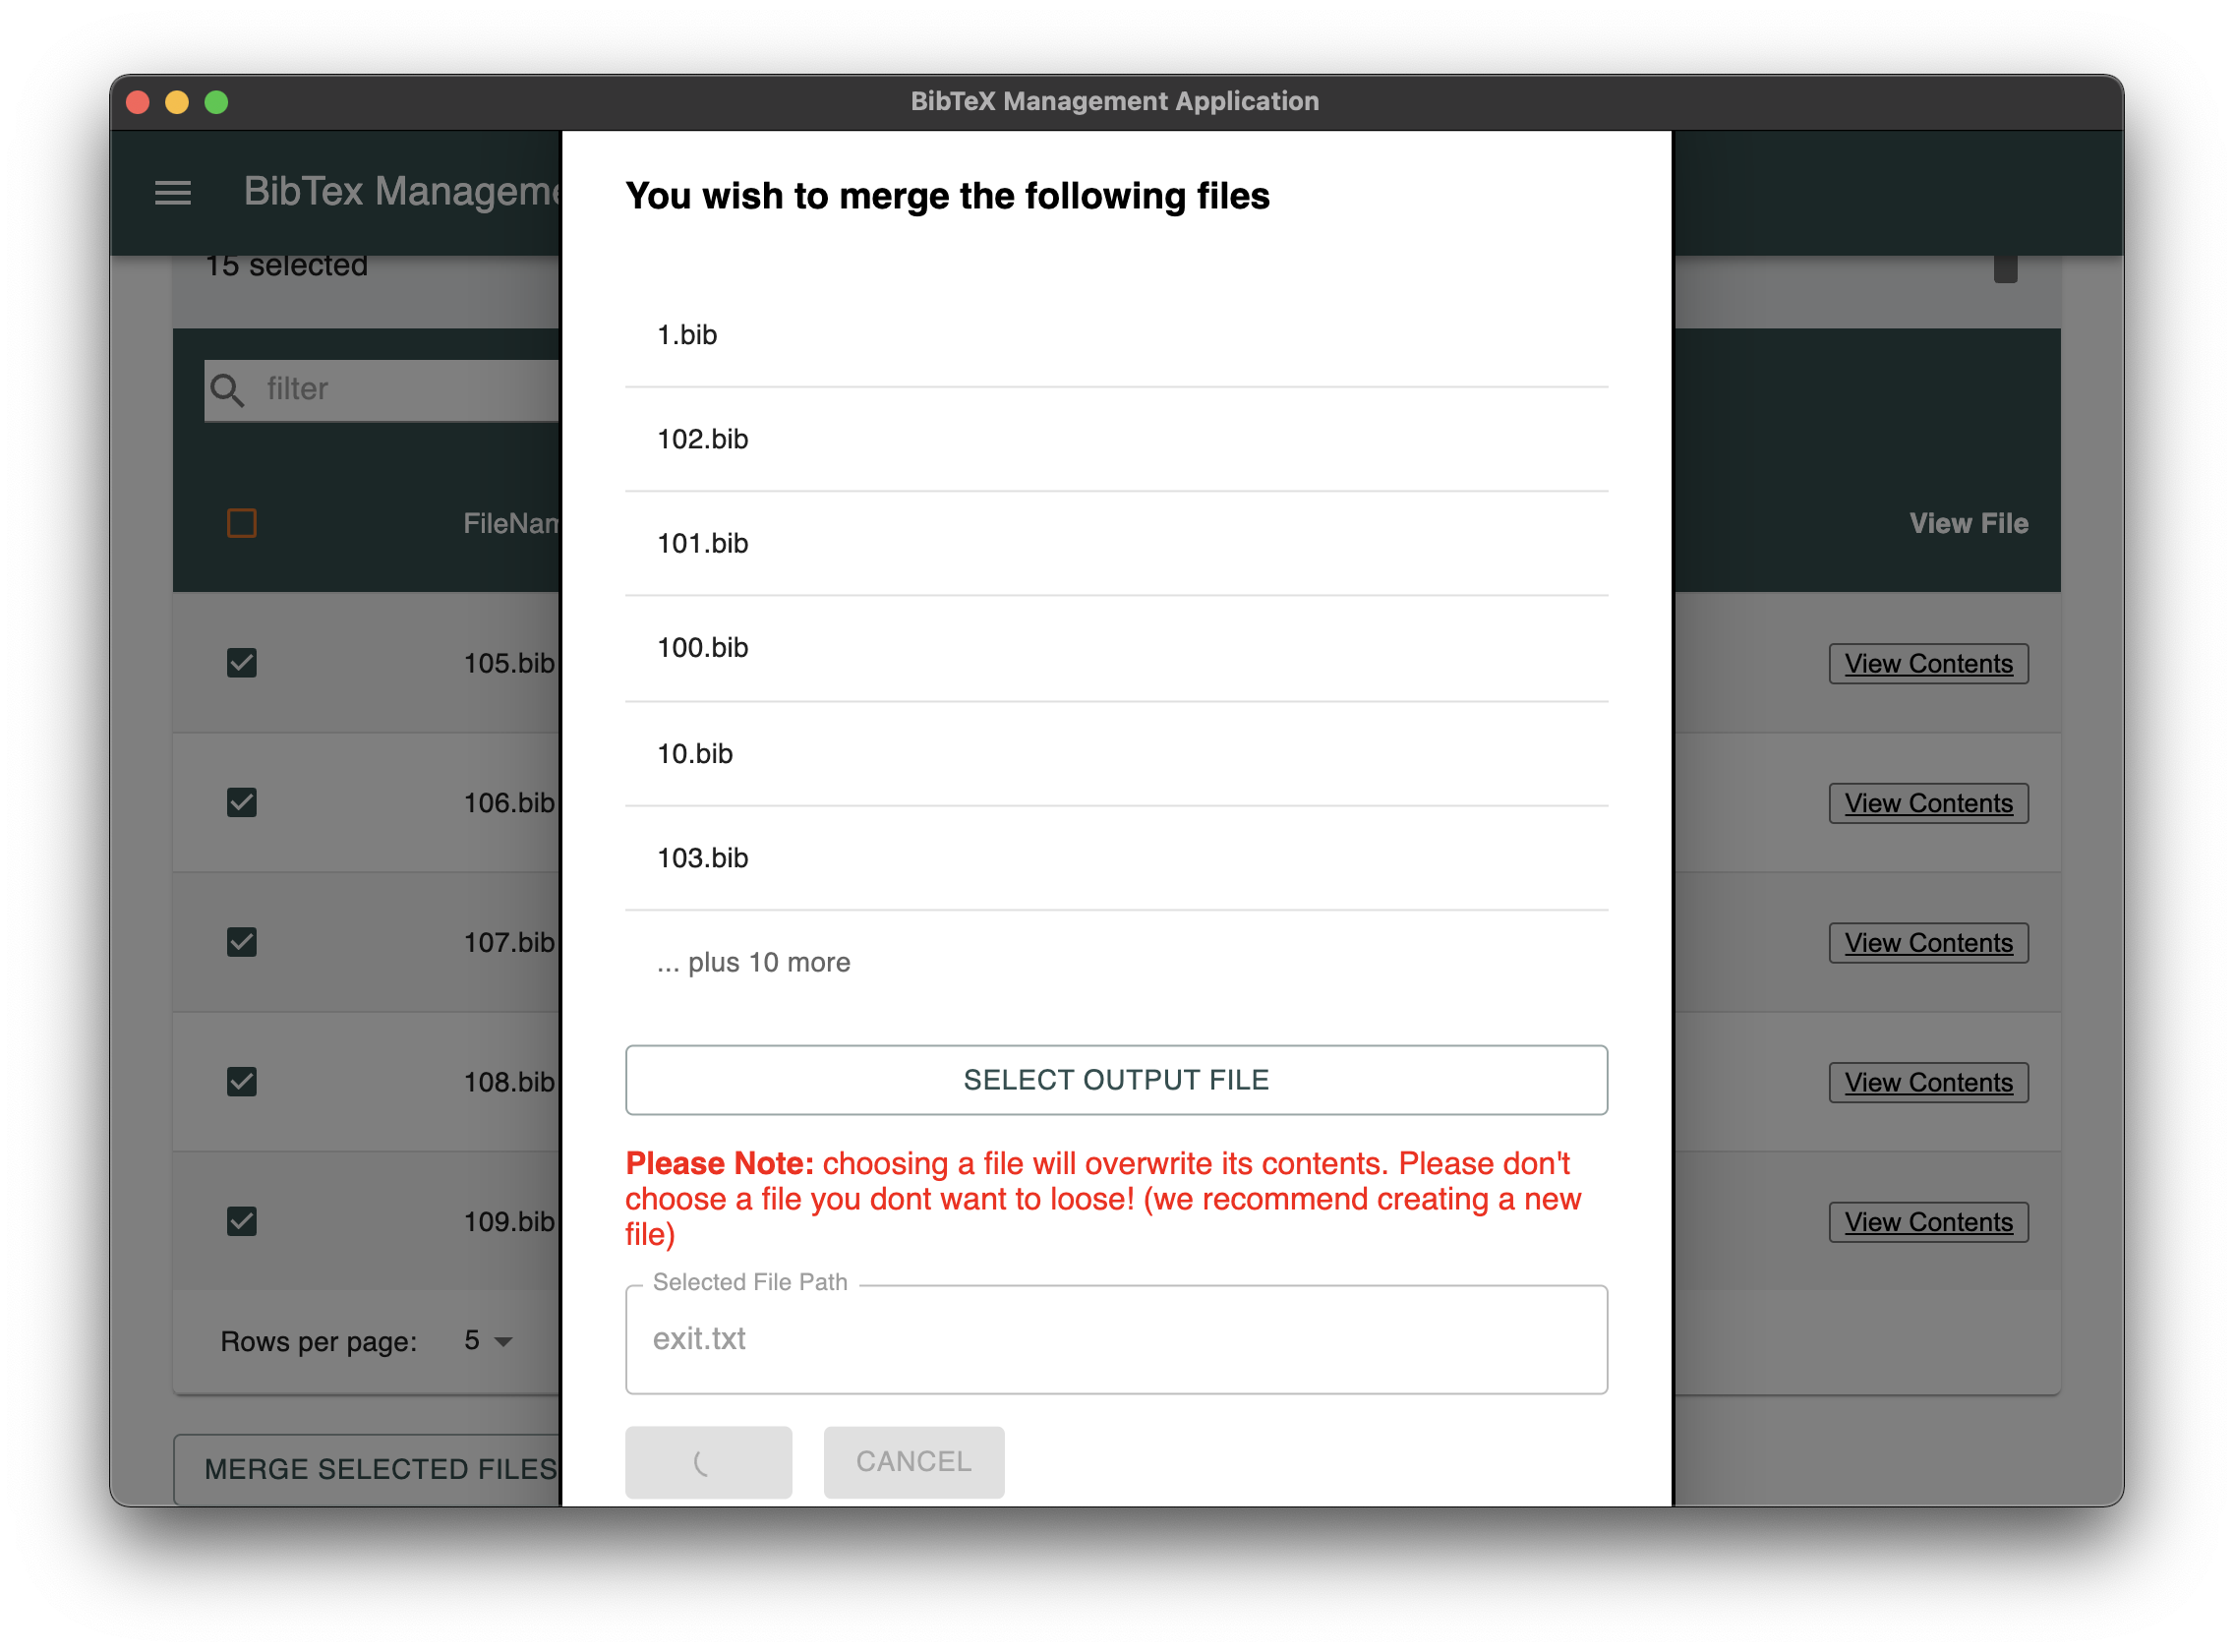
\includegraphics[width=0.8\linewidth]{images/mergingFiles.png}
    \caption{Merging a number of files through the application, demonstrating the loading icon being displayed to the user to show status.}
    \label{fig:mergingFiles}
\end{figure}

It is also worth noting that throughout each of these screens the ability to go back or cancel an operation (except for the merge function once in progress) once in progress is easy to access and visible to the user.

Finally, the application contains an 'Algorithm Sandbox' page. This page allows a user to select a string matching algorithm, enter two strings, then see the comparison score generated by their chosen approximate string matching metric. This has no direct function towards the main goal of the application although was useful within my testing and experimentation of the algorithms I had implemented. It also gives a user the chance to experiment with and understand the underlying algorithm facilitating the operations, as well as the alternative approaches which could be chosen. I did deliberate with allowing the user to choose their matching algorithm on the merge operation, although I felt that this may distract from the core purpose of the application, and especially with the possibly unfamiliar terminology and algorithm names may increase the learning curve for this application. As a result I felt that the addition would be cumbersome for the user and unnecessary. See the algorithm experimentation page in figure \ref{fig:algorithmSandbox}.

\begin{figure}
    \centering
    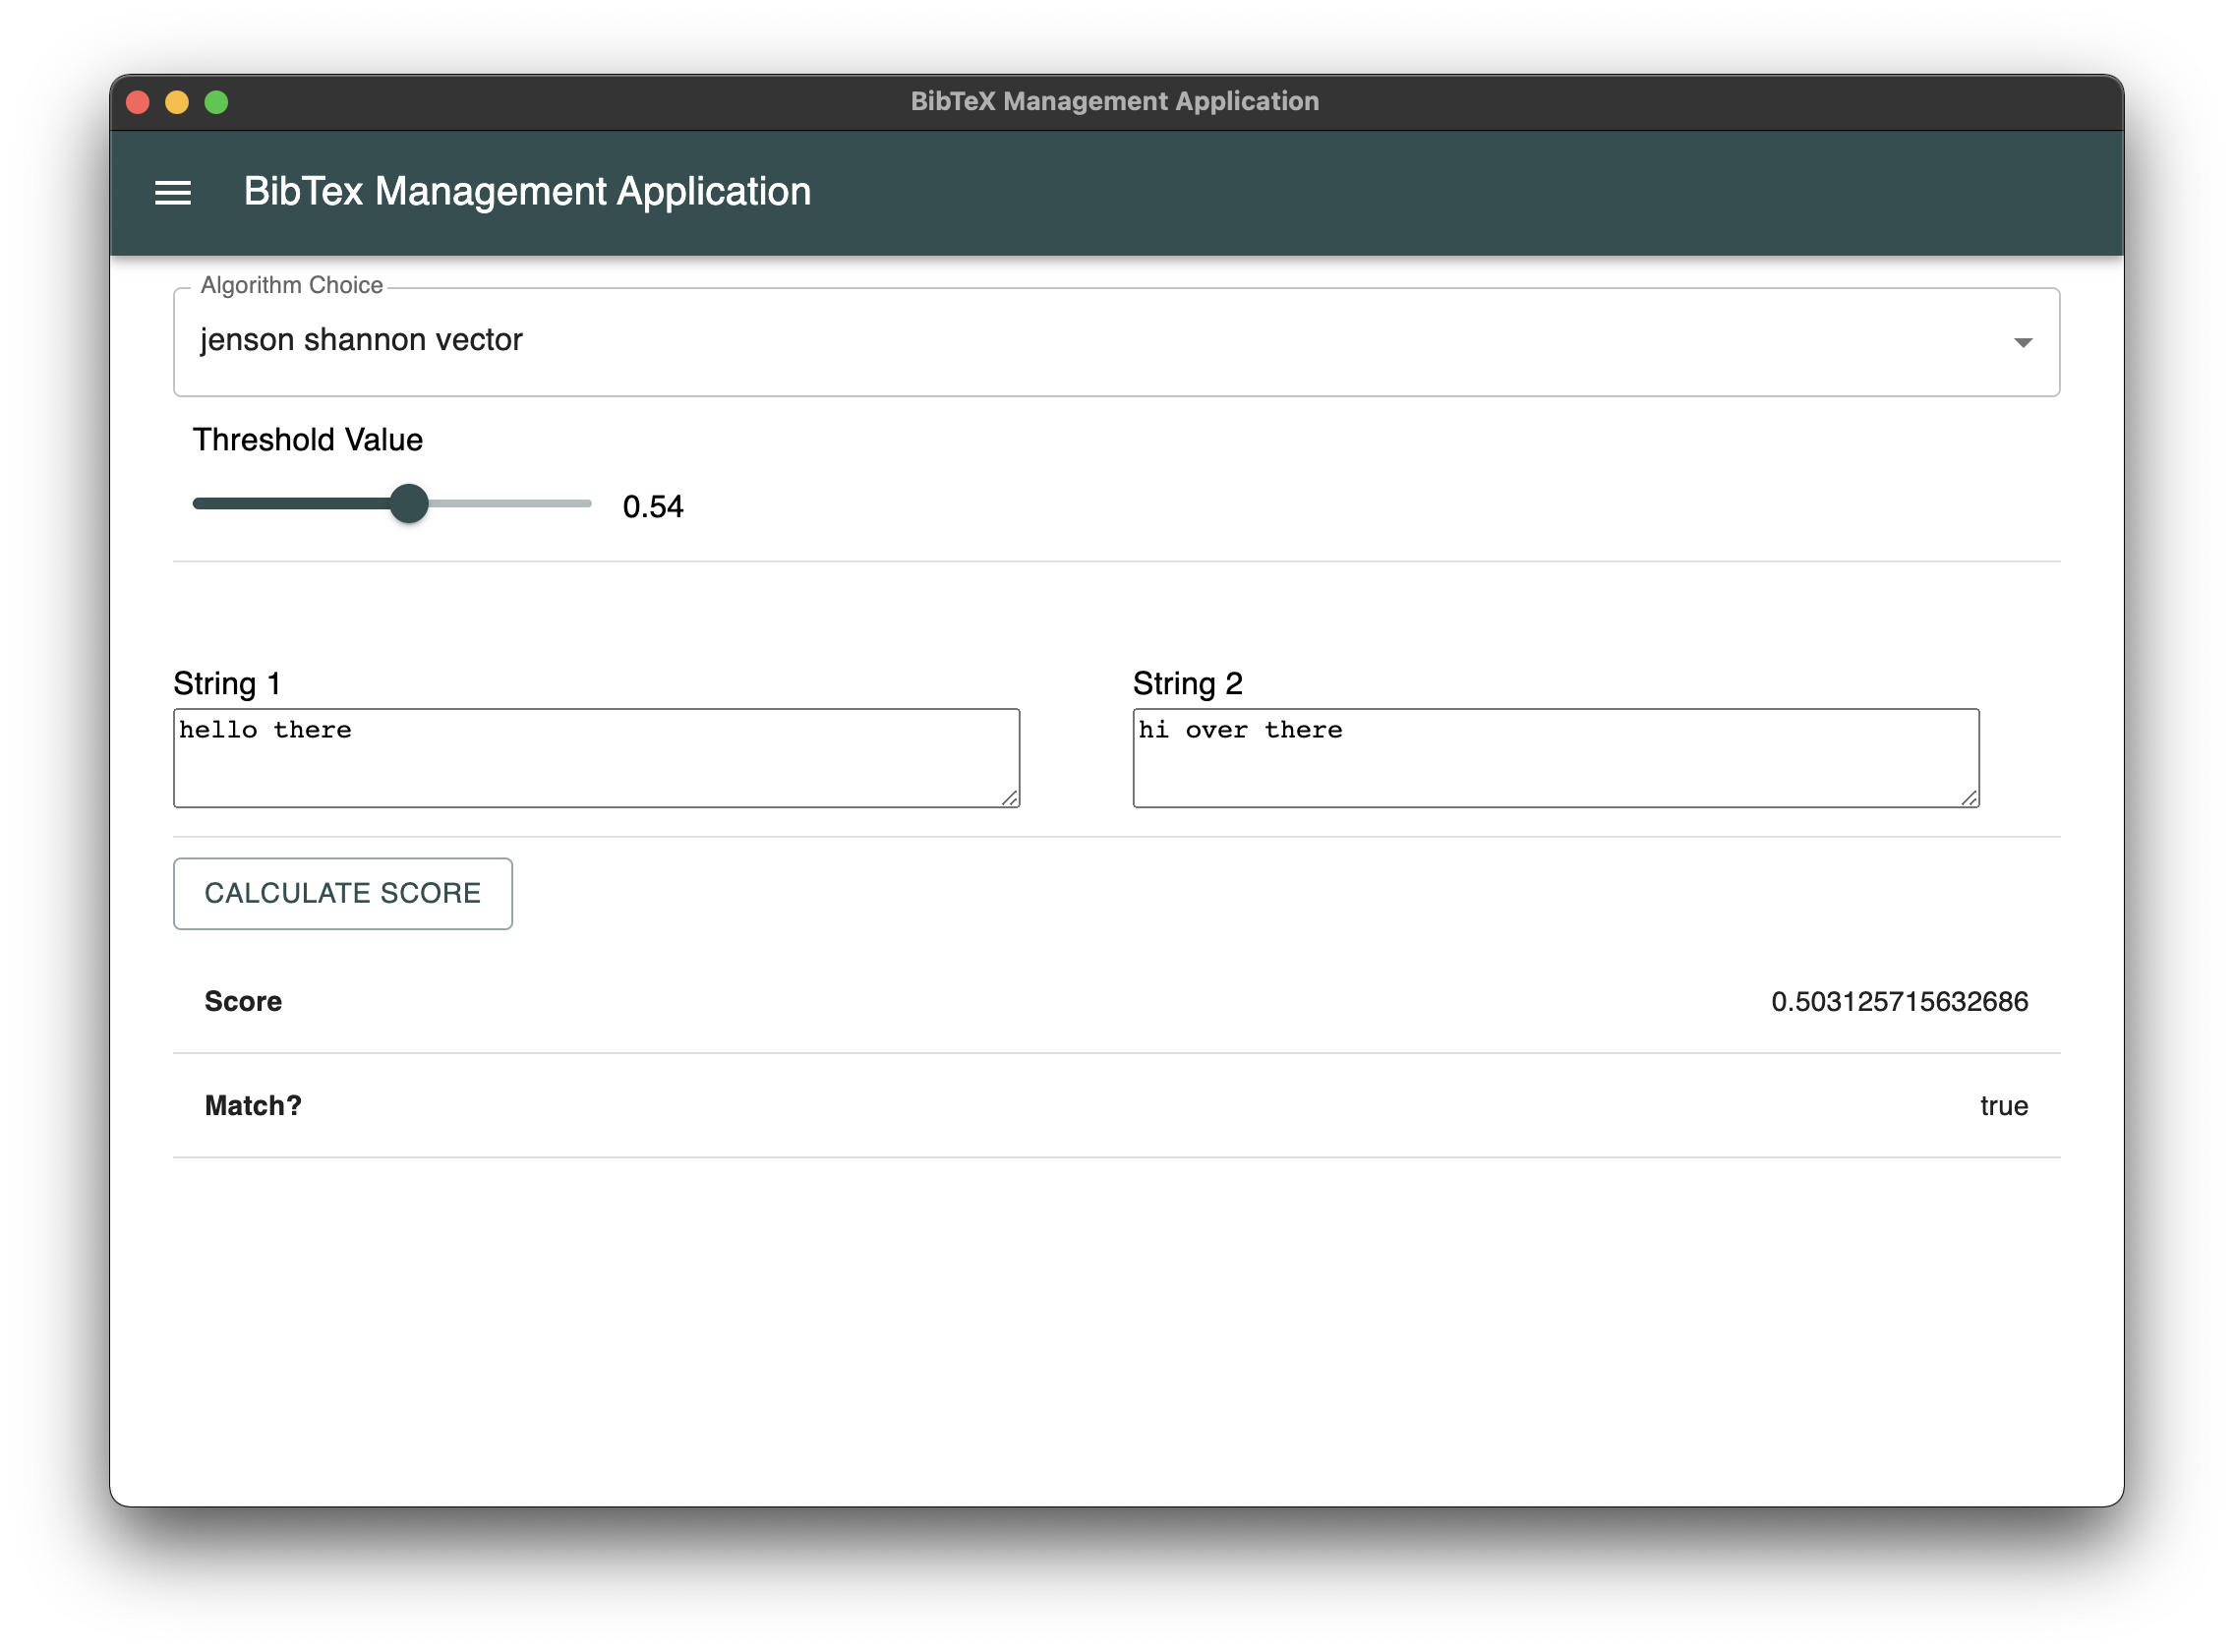
\includegraphics[width=0.8\linewidth]{images/algorithmPlayroom.png}
    \caption{Algorithm sandbox area within the GUI for experimenting with the different algorithms I had implemented}
    \label{fig:algorithmSandbox}
\end{figure}


\section{Evaluation and Critical Appraisal}
\subsection{Primary Objectives}
We can evaluate the work generated during the course of this project and compare it to our laid out requirements, in this report specified in the \textit{requirements specification} section. First of all in that section I described a number of requirements necessary for a minimal viable product (MVP). These requirements I believe have been completed and exceeded. All the capabilities mentioned here are possible and have been extended with other features we have discussed.

From this we can view the rest of the requirements under the \textit{main requirements} group. Once more, all these have been completed. Through the application created for a project a user can search a volume for any BibTeX files, choose the files that they wish to merge, then merge said files. The files are merged whilst removing duplicates, and using an approximate string matching algorithm to find `like' duplicates. This matching algorithm was experimented with to choose one which is near optimal for this context, hence this functionality has been carefully examined and optimised to produce the best results (although possible improvements to this are discussed within the \textit{Future Work} section). I believe doing this extra work to choose such an algorithm was the main interesting takeaway from this project, as well as the way I think this project stands out amongst other work; even other BibTeX management tools.

\subsection{Secondary Objectives}

As for the extension objectives we have made a way through a few of them. Namely, we can now merge a BibTeX file into an existing BibTeX file (rather than creating a new one), we can search through files found on the volume by name, and we can open and view the contents of the BibTeX file within the application GUI. As mentioned in the requirements specification these features are not crucial to the applications main functionality, but improve the usability and functionality of the experience dramatically. Therefore completing these was a good next step in levelling up the application to a higher standard. Several of the other extensions we will discuss further in the following section. Notably the ``multiple user shared citation repository" would bring our application into a new domain, and whilst right now I believe the application solves an unsolved problem, this requirement would be a step towards turning our project more towards being a general citation management tool. Hence, it would be in direct line of competition with the other citation management tools we have mentioned \citep{mendeley, zotero, papersapp}. Thus, although it would be a great next step for the application, it may take the focus away from the main outlined goals of this project.

\subsection{Related Work}

Like the other tools available \citep{mendeley, zotero, papersapp} the project created gives the user a GUI based experience, however I believe whilst those tools each have many merits of their own, the application we have built fills a gap and solves a problem highlighted by my supervisor Richard Connor and others in the initial outline of this project. That problem is the inability to easily and quickly collate a number of BibTeX files into a single, collated file whilst dealing with and removing duplicate entries. I believe that the application we have developed achieves this goal in a sophisticated way, and as a result I would consider this project a success.

This all said, there are issues with the project and features which implemented would enhance the overall experience. First of all, the file selection system can sometimes run into unexpected behaviour when using a combination of the `check all' button and individual file rows. Additionally, there are some problematic CSS scaling issues when the window is shrunk to a small size. Both of these issues are GUI issues which don't impact the overall performance and functionality of the application, but could be improved as quality of life changes. These bugs although small, can separate out our application from the more polished other citation management tools \citep{mendeley, zotero, papersapp}.

The list of successfully implemented features can be found below.

\subsection{Implemented Application Features}

\begin{itemize}
    \item Neon Library Features/Functions
    \begin{itemize}
        \item Through the \code{searchVolume} function our application can search from a given directory through all subdirectories for any files with the \code{.bib} extension, and return them as a list to the user.
        \item Our application can parse a given bib file into a number of BibEntry structs. This can explicitly be performed through the \code{parseBibTeXFile} function.
        \item Our application can parse and merge a number of files into a single output file.
        \item Our application can remove exact duplicates during this merge to prevent them being in the output file.
        \item Implemented several approximate string matching algorithms, namely;
        \begin{itemize}
            \item Hamming Distance
            \item Levenshtein Distance
            \item Wagner Fischer (dynamic programming levenshtein implementation)
            \item Damerau-Levenshtein Distance
            \item Jaro Winkler Distance
            \item Longest Common Subsequence
            \item NGram based distance algorithm
            \item Jensen-Shannon Vector
        \end{itemize}
        \item Our application can use one of the above algorithms to remove near duplicates during the merge process.
    \end{itemize}
    \item GUI Features
    \begin{itemize}
        \item Allows the user to select a directory to search using their native file explorer.
        \item Allows the user to search the selected directory, returning the results.
        \item Shows the user the results of their search in a table format, with pagination.
        \item Allows the user to filter these results to find files of their choosing through a search bar.
        \item Displays to the user information about each found file, such as filename, number of entries and the size of the file.
        \item User can click on a file to view the contents of that file, with the entries formatted into a table.
        \item User can click on a particular entry to view all the field-value pairs in said entry.
        \item Allows the user to select a number of files they wish to merge by clicking on their row (or the checkbox)
        \item Allows the user to merge their selected files, allowing them to choose an output location/file.
        \item User can view an ``Algorithm Sandbox" page where they can experiment with the different algorithms listed above.
    \end{itemize}
\end{itemize}

On top of the implemented features, this project also included a lot of experimental and research work surrounding the different approximate string matching algorithms implemented. As a result, one of the great successes of this project was also developing a deeper understanding of these algorithms as well as the surrounding work and history of the field of approximate string matching algorithms.

\section{Future Work}
There are several directions with which this application could be taken. That said, before the algorithm moves towards new functionality, there are a number of things which could be done to improve existing functionality.

First of all, the GUI could be expanded upon to provide more status information to the user, such as progress bars for certain operations. Additionally, although the complexity of the implemented algorithms is well understood and documented, we could improve the efficiency of the application through other means. The first example is by utilising concurrency to perform the computationally expensive operations, such as performing matching checking over a large set of files/entries. Our application is already in a good stand point to move across to this due to our decision to implement these operations in rust; a language with very good concurrency features and support.

Furthermore, other techniques could be examined to leverage and improve the approximate string matching. For example using machine learning based techniques. This paper \citep{mlStringMatching} describes how techniques have been developed within the machine learning domain to map text to a low dimensional continuous vector space using deep learning approaches.

We could also begin to expand our feature set; I mentioned earlier that the application could move towards being a more general purpose citation management tool. Features such as being able to maintain a repository of citations/files, edit files within the GUI, and network capabilities in order to be able to work collaboratively would all help achieve this. As mentioned this work would `level-up' the application, but also bring it into the domain and in direct competition of other general citation management tools. As it stands right now this application is novel and provides new functionality, rather than trying to influence and improve existing solutions.

\section{Conclusion}
The outward goal of this project was to provide a solution to a problem currently unsolved by existing citation management tools; the inability to easily and quickly collate a number of BibTeX files into a single, collated file whilst dealing with and removing duplicate entries. As discussed in the evaluation section, I believe that the application I have created provides a solution to this problem.

Alongside solving this issue, there were a few key successes of the project to take away from this. The first, and where the bulk of the work for this project lay, was developing a deeper understanding of the research area of approximate string matching algorithms. Through both theoretical, experimental and practical analysis we understood and implemented a range of these algorithms with varying degrees of complexity. Using these findings we then applied our understanding to choose the algorithm best suited to the context of our application. That said, this area of research is decades old and still expanding today, so although clear progress and understanding has progressed throughout this project, the scope for expansion is enormous. There is much more learning and many more techniques which could be experimented with if we were to choose to take this further.

The structure of this application had many moving components and required a range of technologies and skillsets in order to successfully complete. I believe that considering these factors we have executed an application covering a range of technologies which meets the criteria we laid out in our specification. The product we have delivered well fulfils these requirements, and I believe that the scope of our applications domain allowed us to focus on fulfilling these fewer requirements to a high standard, rather than ``spreading ourselves to thin". That said, we've discussed in the \textit{Evaluation and Critical Appraisal} and \textit{future work} sections several areas in which we could improve our work, or described new features which could be added to enhance user experience and/or provide more functionality.

Overall I have learnt a lot in this project and thoroughly enjoyed working in the technology stack I chose. The experimentation I have done has not only taught me a lot about the algorithms I have worked with, but as also demonstrated how theoretical analysis and experimentation with theories such as computational complexity can have real life application. This shows how findings discovered through these means can be deployed to make the best decision on how to implement a piece of functionality.
\newpage
\bibliography{bib}

\appendix

\section{Additional Figures}
\begin{figure}[H]
    \centering
    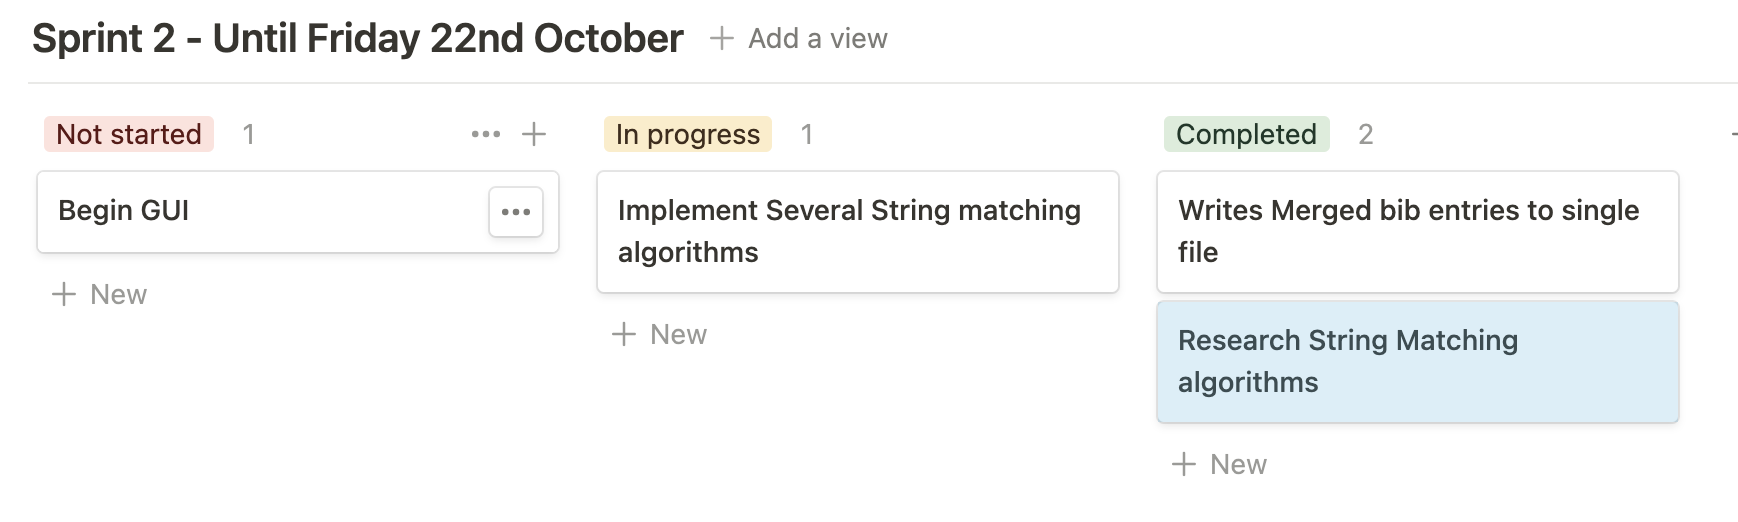
\includegraphics[width=\linewidth]{images/kanbanBoard.png}
    \caption{Kanban board for the second sprint (note stories progress statuses have been adjusted to represent how the board would have appeared mid sprint)}
    \label{fig:kanbanBoard}
\end{figure}

\section{Testing}
\subsection{Parsing}
Testing was done through feeding the parsing algorithms BibTeX files and cross-checking the struct data outputs against those expected from the input files. Error cases were manually created from these files and checked for handling within the program.

My supervisor Richard Connor was also kind enough to send me over 120 BibTeX files from work he had produced, all of these a mixture of files manually created by himself, or generated by alternative citation management tools. Despite these conditions many of these BibTeX files were not valid BibTeX files! Thus the scale of this data to test the algorithms produced a solid testing suite for the parsing algorithms implemented, covering a wide range of error cases.

\subsection{Algorithms}
Algorithms were tested via a range of values being given to each algorithm. This included erroneous and edge cases such as empty strings, strings of alternative length, and for some algorithms extensively long strings to check for runtime errors such as Stack Overflows.

The results were cross checked against existing implementations for the algorithms and, where those were not available, the value was occasionally calculated by hand to ensure consistency.

\subsection{Merging}
Merging once again was tested through the large scale data set of BibTeX algorithms provided by Richard Connor. Cases such as exact duplicates and near duplicates were manufactured to ensure that they were removed during the merge process. An expansion on this if we were to move towards a production deployment would be to integrate Unit testing into the framework to test this functionality.

\subsection{GUI Testing}
The GUI was tested manually by running through the various routes possible for a user to access, attempting to access erroneous states etc. An expansion given more time on this project would be to utilise a GUI testing framework such as ``Cyprus" to ensure the operations performable on the frontend followed expected behaviour.

\section{User Manual}
The project directory has the following structure:
\begin{itemize}
    \item \code{\textbf{/data}}
    \item \code{\textbf{/frontend}}
    \item \code{\textbf{/implementation}}
    \item \code{\textbf{/native}}
    \item \code{\textbf{/testBibFiles}}
    \item \code{algorithm\textunderscore comparison\textunderscore script.js}
    \item \code{test\textunderscore script.js}
    \item \code{README.md}
    \item \code{package.json}
\end{itemize}
The README.md file contains instructions about building and running the program. The contents of this are copied in the document below.

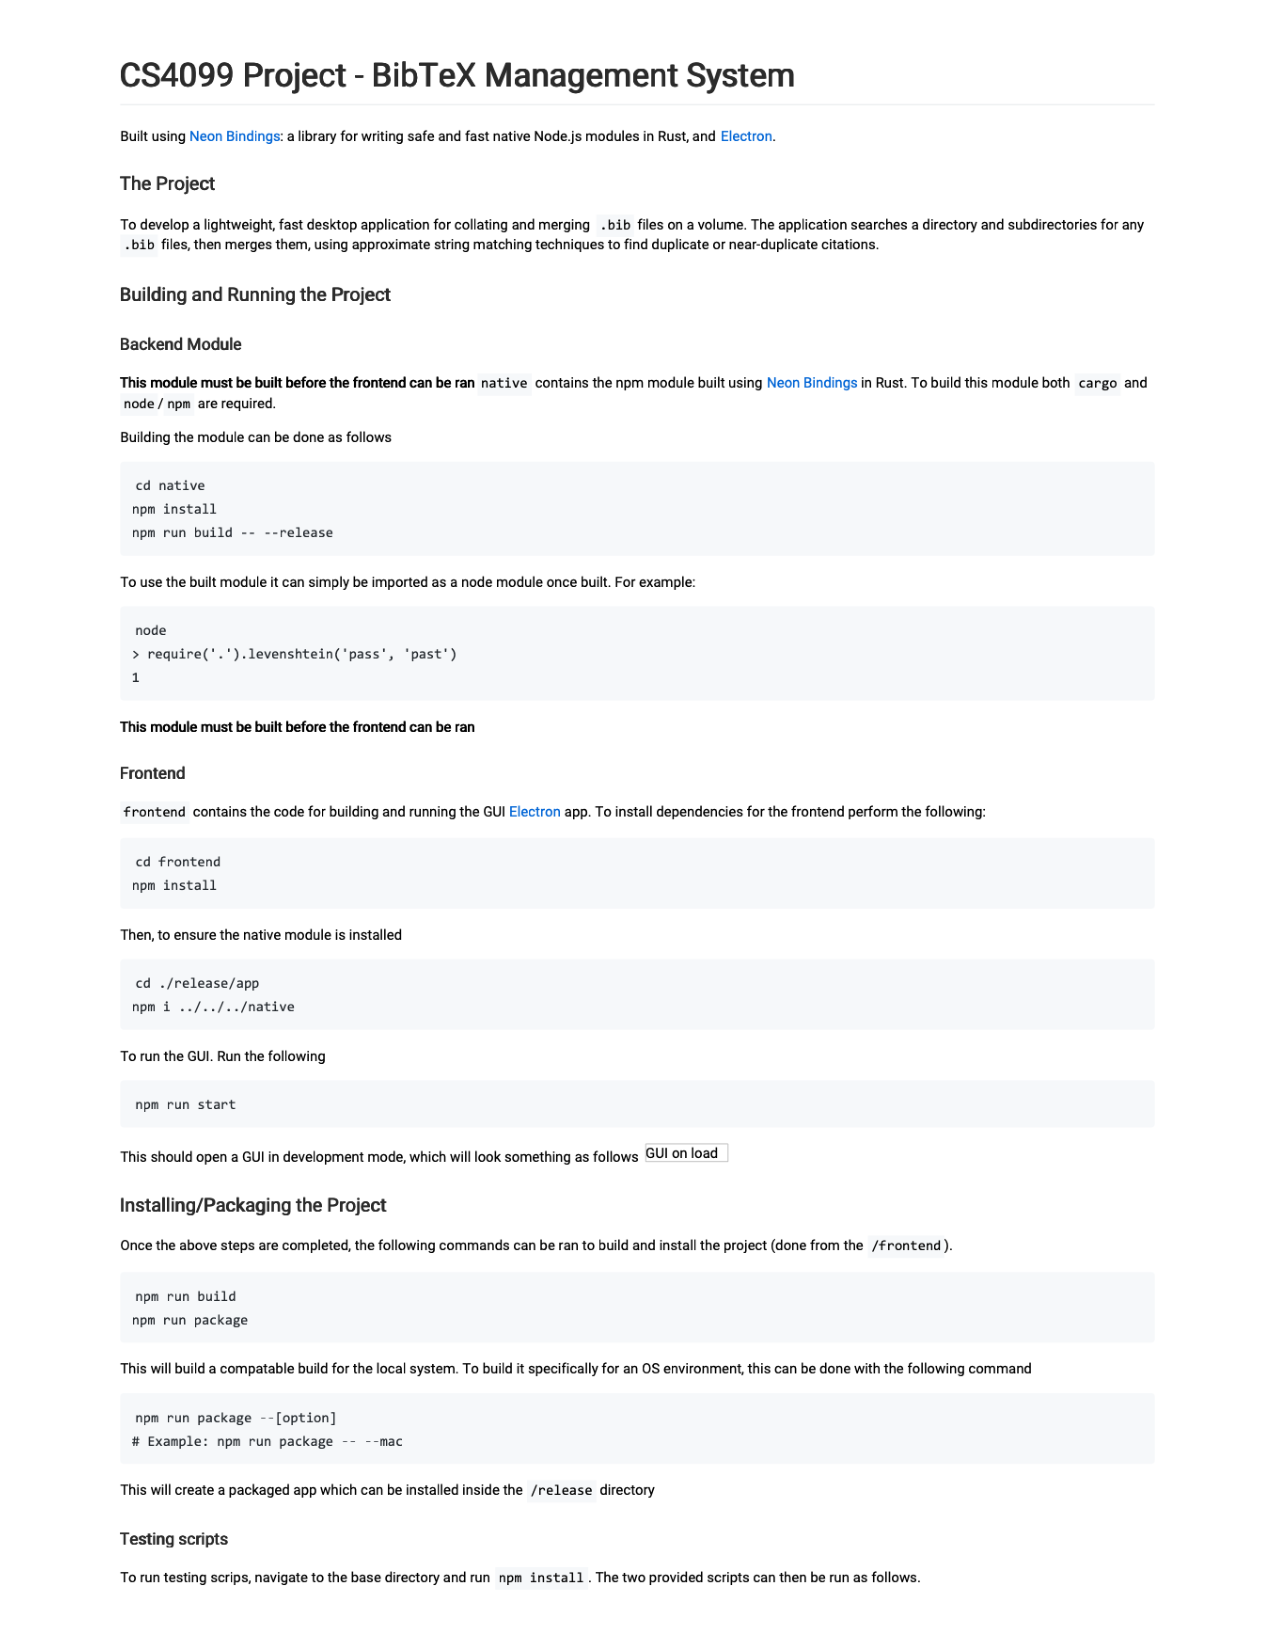
\includepdf[pages=-,pagecommand={},width=1.2\textwidth]{README.pdf}

\section{Additional Test Results Data}\label{appendix:testdata}

\begin{table}[H]
      \centering
      \begin{tabular}{|c|p{0.9\textwidth}|}
      \hline
           Number &  String \\ \hline \hline
           1 & "Richard Connor and Alan Dearle and Lucia Vadicamo" \\ \hline
           2 & "\{R. Connor\} and \{A. Dearle\} and \{L. Vadicamo\}" \\ \hline
           3 & "Connor, Richard and Dearle, Alan and Vadicamo, Lucia" \\ \hline
           4 & "\{R. Connor, A. Dearle, and L. Vadicamo\}" \\
           \hline
      \end{tabular}
  \caption{Strings being used to compare group 2 of like BibTeX entry authors}
\label{table:authorsGroup2Strings}
\end{table}
    \begin{table}[H]
    \centering
       \begin{tabular}{|c|c|c|c|c|}
    \hline
     & \multicolumn{4}{c|}{Algorithm Score (Time taken in ms in bracket)}\\
     \hline
     Compared Strings  & Wagner-Fischer & Jaro-Winkler & n-gram (2) & Jensen-Shannon \\
     \hline \hline
    1,2 & 19 (7.63) & 0.652 (5.21) & 0.327 (0.680) & 0.472 (0.709) \\
             \hline
    1,3 & 33 (9.36) &
0.600 (5.95 &)
0.500 (0.762) &
0.255 (0.777)\\
    \hline
    1,4 & 20 (6.22) &
0.635 (3.93) &
0.327 (0.618) &
0.457 (0.690) \\
    \hline
    \end{tabular}
    \caption{Score results (note lower score indicates more similar) of author group 2 strings compared to each other using Wagner-Fischer, Jaro-Winkler, n-gram and Jensen Shannon, using strings from table \ref{table:authorsGroup2Strings}}
\label{table:algComparisonResultsAuthor2}
\end{table}

\begin{table}[H]
      \centering
      \begin{tabular}{|c|p{0.9\textwidth}|}
      \hline
           Number &  String \\ \hline \hline
           1 & "Turing, Alan M" \\ \hline
           2 & "\{A. M. Turing\}" \\ \hline
           3 & "Alan M Turing" \\ \hline
      \end{tabular}
  \caption{Strings being used to compare group 3 of like BibTeX entry authors}
\label{table:authorsGroup3Strings}
\end{table}
    \begin{table}[H]
    \centering
       \begin{tabular}{|c|c|c|c|c|}
    \hline
     & \multicolumn{4}{c|}{Algorithm Score (Time taken in ms in bracket)}\\
     \hline
     Compared Strings  & Wagner-Fischer & Jaro-Winkler & n-gram (2) & Jensen-Shannon \\
     \hline \hline
    1,2 & 13 (0.272) &
0.618 (0.136) &
0.786 (0.0712) &
0.612 (0.155) \\
             \hline
    1,3 & 12 (0.246) &
0.616 (0.125) &
0.643 (0.0668) &
0.342 (0.151) \\
    \hline
    \end{tabular}
    \caption{Score results (note lower score indicates more similar) of author group 3 strings compared to each other using Wagner-Fischer, Jaro-Winkler, n-gram and Jensen Shannon, using strings from table \ref{table:authorsGroup3Strings}}
\label{table:algComparisonResultsAuthor3}
\end{table}

\begin{table}[H]
      \centering
      \begin{tabular}{|c|p{0.9\textwidth}|}
      \hline
           Number &  String \\ \hline \hline
           1 & "Albert Einstein" \\ \hline
           2 & "Albert Einstien" \\ \hline
           3 & "Alborto Entien" \\ \hline
      \end{tabular}
  \caption{Strings being used to compare group 4 of like BibTeX entry authors}
\label{table:authorsGroup4Strings}
\end{table}
    \begin{table}[H]
    \centering
       \begin{tabular}{|c|c|c|c|c|}
    \hline
     & \multicolumn{4}{c|}{Algorithm Score (Time taken in ms in bracket)}\\
     \hline
     Compared Strings  & Wagner-Fischer & Jaro-Winkler & n-gram (2) & Jensen-Shannon \\
     \hline \hline
    1,2 & 2 (0.325) &
0.0522 (0.0550) &
0.0667 (0.0820) &
0.236 (0.170) \\
             \hline
    1,3 & 6 (0.292) &
0.343 (0.106) &
0.267 (0.0738) &
0.534 (0.166) \\
    \hline
    \end{tabular}
    \caption{Score results (note lower score indicates more similar) of author group 4 strings compared to each other using Wagner-Fischer, Jaro-Winkler, n-gram and Jensen Shannon, using strings from table \ref{table:authorsGroup4Strings}}
\label{table:algComparisonResultsAuthor4}
\end{table}

\begin{table}[H]
      \centering
      \begin{tabular}{|c|p{0.9\textwidth}|}
      \hline
           Number &  String \\ \hline \hline
           1 & "Modelling \{String\} \{Structure\} in \{Vector\} \{Spaces\}" \\ \hline
           2 & "Modelling \{S\}tring \{S\}tructure in \{V\}ector \{S\}paces" \\ \hline
           3 & "\{Modelling String Structure in Vector Spaces\}" \\ \hline
           4 & "modelling string structure in vector spaces" \\ \hline
      \end{tabular}
  \caption{Strings being used to compare group 2 of like BibTeX entry titles}
\label{table:titleGroup2Strings}
\end{table}
    \begin{table}[H]
    \centering
       \begin{tabular}{|c|c|c|c|c|}
    \hline
     & \multicolumn{4}{c|}{Algorithm Score (Time taken in ms in bracket)}\\
     \hline
     Compared Strings  & Wagner-Fischer & Jaro-Winkler & n-gram (2) & Jensen-Shannon \\
     \hline \hline
    1,2 & 8	(9.65) &
0.352 (4.12) &
0.157 (0.766) &
0.274 (0.781) \\
             \hline
    1,3 & 8 (8.04) &
0.554 (4.91) &
0.157 (0.691) &
0.292 (0.718) \\
    \hline
    1,4 & 13 (7.66) &
0.523 (4.75) &
0.176 (0.687) &
0.494 (0.696) \\
    \hline
    \end{tabular}
    \caption{Score results (note lower score indicates more similar) of title group 2 strings compared to each other using Wagner-Fischer, Jaro-Winkler, n-gram and Jensen Shannon, using strings from table \ref{table:titleGroup2Strings}}
\label{table:algComparisonResultsTitle2}
\end{table}

\begin{table}[H]
      \centering
      \begin{tabular}{|c|p{0.9\textwidth}|}
      \hline
           Number &  String \\ \hline \hline
           1 & "Computing Patterns In Strings" \\ \hline
           2 & "Computing Patturns In Strings" \\ \hline
           3 & "cmputing patterns in strngs" \\ \hline
      \end{tabular}
  \caption{Strings being used to compare group 3 of like BibTeX entry titles}
\label{table:titleGroup3Strings}
\end{table}
    \begin{table}[H]
    \centering
       \begin{tabular}{|c|c|c|c|c|}
    \hline
     & \multicolumn{4}{c|}{Algorithm Score (Time taken in ms in bracket)}\\
     \hline
     Compared Strings  & Wagner-Fischer & Jaro-Winkler & n-gram (2) & Jensen-Shannon \\
     \hline \hline
    1,2 & 1 (1.95) &
0.0126 (0.119) &
0.00 (0.266) &
0.191 (0.376) \\
             \hline
    1,3 & 6 (1.76) &
0.642 (1.10) &
0.103 (0.256) &
0.432 (0.350) \\
    \hline
    \end{tabular}
    \caption{Score results (note lower score indicates more similar) of title group 3 strings compared to each other using Wagner-Fischer, Jaro-Winkler, n-gram and Jensen Shannon, using strings from table \ref{table:titleGroup3Strings}}
\label{table:algComparisonResultsTitle3}
\end{table}

\section{Artifact Evaluation Form}

\includepdf[pages=-,pagecommand={},width=\textwidth]{CS_Artifact_evaluation_form_2020_21.pdf}

\end{document}
